\documentclass[a4paper]{article}
\usepackage{header}


\title{\HugeЛинейная алгебра}
\author{
	Бобень Вячеслав, Сиренева Ника \\
	\href{https://teleg.run/darkkeks}{@darkkeks},
    \href{https://t.me/nih3kwo}{@nih3kwo},
    \href{https://github.com/LoDThe/hse-tex}{GitHub}\\
    Благодарность выражается Левину Александру (\href{https://teleg.run/azerty0123456789}{@azerty1234567890}) и Милько Андрею \\
    (\href{https://teleg.run/andrew_milko}{@andrew\_milko}) за видеозаписи лекций.
}
\date{2024 --- 2025}

\begin{document}
    \maketitle

    \begin{center}
        Дисклеймер: с 19 лекции конспект может содержать большее количество ошибок, так как обновился недавно. Просьба сообщить о них в issues или самим исправить их в pull requests.
    \end{center}

    \epigraph{
        ``К коллоку можете даже не готовиться''.
    }{\rightline{{\rm --- Роман Сергеевич Авдеев}}}

    \tableofcontents

    \newpage

    \section{Кратные интегралы. Брусы. Интегрируемые функции по Риману}

\subsection{Брус. Мера бруса}

\definition Замкнутый брус (координатный промежуток) в $\mathbb{R}^n$ — множество, описываемое как



\begin{equation*}
\begin{aligned}
    I&=\{x\in\mathbb{R}^n\ |\ a_i\leq x_i\leq b_i,\ i\in\{1,n\}\}\\
    &=\left[a_1,b_1\right]\times\ldots\times\left[a_n,b_n\right]
\end{aligned}
\end{equation*}

\comment $I=\{a_1,b_1\}\times\ldots\times\{a_n,b_n\}$, где $\{a_i, b_i\}$ может быть отрезком, интервалом и т.д.

\begin{center}
    % \documentclass[a4paper]{article}
% \usepackage[english,russian]{babel}
%
%
% \usepackage{tikz}
\usetikzlibrary{arrows.meta, 3d, perspective}
% \begin{document}

\begin{tikzpicture}[
    set/.style={dashed, thick},
    arrow/.style={-{Stealth[scale=1.2]}, thick}
]


\def\a{2} % длина
\def\b{2} % ширина
\def\c{2} % высота

    % Координаты вершин куба
\coordinate (A) at (0,0,0);
\coordinate (B) at (\a,0,0);
\coordinate (C) at (\a,\b,0);
\coordinate (D) at (0,\b,0);
\coordinate (E) at (0,0,\c);
\coordinate (F) at (\a,0,\c);
\coordinate (G) at (\a,\b,\c);
\coordinate (H) at (0,\b,\c);

    % Рисуем невидимые ребра (пунктиром)
\draw[dashed] (A) -- (D);
\draw[dashed] (A) -- (B);
\draw[dashed] (A) -- (E);

    % Рисуем видимые ребра
\draw (B) -- (C) -- (G) -- (F) -- (B);
\draw (D) -- (H);
\draw (C) -- (D);
\draw (F) -- (G) -- (H) -- (E) -- (F);

\draw[<->,thick] (0.2, 0, \c + 0.5) -- node[below] {$[a_1 ; b_1]$} (\a + 0.1, 0, \c + 0.5);

\draw[<->,thick] (\a + 0.2, 0.1, 0) -- node[below,rotate=90] {$[a_3 ; b_3]$} (\a + 0.2, \b, 0);

\draw[<->,thick] (\a + 0.2, 0, \c) -- node[below,sloped] {$[a_2 ; b_2]$} (\a + 0.2, 0, \c - 1.8);


\draw (-5, -0.8) rectangle (-3, 1.2);
\draw[<->,thick] (-5, -1) to (-3, -1);
\node at (-4, -1.3) {$[a_1 ; b_1]$};
\draw[<->,thick] (-2.8, 1.2) to (-2.8, -0.8);
\node[rotate=90] at (-2.4, 0.2) {$[a_2 ; b_2]$};

\draw[|-|] (-9, 0.2) to (-7, 0.2);
\draw[<->,thick] (-9, -0.1) to (-7, -0.1);
\node at (-8, -0.4) {$[a_1 ; b_1]$};



\node[align=center] at (-4,-2) {Пример брусов размерности с 1 по 3};

\end{tikzpicture}


% \end{document}

\end{center}

\definition Мера бруса — его объём:

\begin{equation*}
    \begin{aligned}
        \mu(I)&=|I|
        =\prod_{i=1}^{n} (b_i-a_i)
    \end{aligned}
\end{equation*}

\subsection{Свойства меры бруса в $\R^n$}

\begin{enumerate}
    \item \textbf{Однородность:} $\mu(I_{\lambda a,\lambda b})=\lambda^n\cdot\mu(I_{a,b})$, где $\lambda\geq
    0$
    \item \textbf{Аддитивность:} Пусть $I, I_1, \ldots, I_k$ — брусы
    
    Тогда, если $\forall i, j\, I_i, I_j$ не имеют общих внтренних точек, и $\displaystyle\bigcup_{i=1}^kI_i = I$, то
    $$|I| = \sum_{i=1}^k|I_i|$$
    \item \textbf{Монотонность}: Пусть $I$ — брус, покрытый конечной системой брусов, то есть $I\subset \displaystyle\bigcup_{i=1}^kI_i$, тогда
    $$|I| < \sum_{i=1}^k|I_i|$$
\end{enumerate}

\subsection{Разбиение бруса. Диаметр множества. Масштаб разбиения}

\definition \label{1.3} $I$ — замкнутый, невырожденный брус и $\displaystyle\bigcup_{i=1}^kI_i = I$, где $I_i$ попарно не имеют общих внутренних точек. Тогда набор $\T = \{\T\}_{i=1}^k$ называется разбиением бруса $I$

\definition \label{1.4} Диаметр произвольного ограниченного множества $M\subset\R^n$ будем называть 

\begin{equation*}
\begin{aligned}
    d(M) = \displaystyle\sup_{1\leq i\leq k}\|x-y\|,\text{ где}\\
    \|x-y\|=\sqrt{\sum_{i=1}^{n}\left(x_i-y_i\right)^2}
\end{aligned}
\end{equation*}

\begin{center}
    % \documentclass[a4paper]{article}
% \usepackage[english,russian]{babel}
%
%
% \usepackage{tikz}
% \usetikzlibrary{arrows.meta}
% \begin{document}

\begin{tikzpicture}[
    set/.style={dashed, thick},
    arrow/.style={-{Stealth[scale=1.2]}, thick}
]

\draw (-4, 0) circle (40pt);
\draw[latex-latex, line width=1pt] (-3, -1) -- (-5, 1);
\node[rotate=-45] at (0.2, 0.2) {d};

\draw[set] (0, 0) circle (40pt);
\draw[latex-latex, line width=1pt] (1, -1) -- (-1, 1);
\node[rotate=-45] at (-3.8, 0.2) {d};

\fill (3, 1.3) circle (1.75pt);
\fill (4, 0) circle (1.75pt);
\fill (5, -1.3) circle (1.75pt);
\draw[latex-latex, line width=1pt] (5.15, -1.2) -- (3.15, 1.4);
\draw[Bar-Bar, line width=0.7pt] (5.15, -1.2) -- (3.15, 1.4);
\node[rotate=-55] at (4.4, 0.2) {d};

\node[align=center] at (0,-2) {Пример диаметра для разных ограниченных множеств(Для всех трёх он равен $d$)};

\end{tikzpicture}


% \end{document}

\end{center}


\definition \label{1.5} Масштаб разбиения $\T=\{I_i\}_{i=1}^k$ — число $\lambda(\T) = \Delta_{\T} = \displaystyle\max_{1\le i\le k} d(I_i)$

\definition \label{1.6} Пусть $\forall\ I_i$ выбрана точка $\xi_i\in I_i$. Тогда, набор $\xi = \{\xi_i\}_{i=1}^k$ будем называть \textbf{отмеченными точками}

\definition \label{1.7} Размеченное разбиение — пара $(\T, \xi)$

\subsection{Интегральная сумма Римана. Интегрируемость по Риману}
Пусть $I$ — невырожденный, замкнутый брус, функция $f: I\rightarrow \R$ определена на $I$

\definition \label{1.8} Интегральная сумма Римана функции $f$ на $(\T, \xi)$ — величина
$$\sigma(f, \T, \xi) := \sum_{i=1}^kf(\xi_i)\cdot|I_i|$$

\definition \label{1.9} Функция $f$ интегрируема (по Риману) на замкнутом брусе $I$ ($f:I\rightarrow\R$), если 

\begin{equation*}
\begin{aligned}
    \exists A\in\R: \forall \varepsilon > 0\, \exists \delta > 0: \forall(\T, \xi): \Delta_{\T} < \delta:\\
    |\sigma(f, \T, \xi)| - A| < \varepsilon
\end{aligned}
\end{equation*}

Тогда 
$$A = \int\limits_If(x)\d{x} = \underset{I}{\int\ldots\int}f(x_1, \ldots, x_n)\d{x_1}\ldots \d{x_n}$$
Обозначение: $f\in\mathcal{R}(I)$

\begin{center}
    % \documentclass[tikz,border=5pt]{standalone}
% \usepackage{pgfplots}
\pgfplotsset{compat=newest}
% \usepackage[english,russian]{babel}

% \begin{document}
\begin{tikzpicture}
  \begin{axis}[
    view={120}{30}, % угол обзора
    axis lines=center,
    xlabel={$x$}, ylabel={$y$}, zlabel={$z$},
    ticks=none,
    domain=0:1, y domain=0:1,
    samples=31, samples y=31,
    colormap/viridis,
    zmax=0.8, zmin=0,
    xmin=0, xmax=1.2,
    ymin=0, ymax=1.2
  ]

  % поверхность f(x,y) = 0.4 + 0.2*sin(2*pi*x)*cos(2*pi*y)
  \addplot3[surf, opacity=0.7]
    {0.6 + 0.05*sin(deg(2*pi*x))*cos(deg(2*pi*y))};

  % сетка внизу
  \foreach \i in {0,0.2,...,1} {
    \addplot3[black, thin] coordinates {(\i,0,0) (\i,1,0)};
    \addplot3[black, thin] coordinates {(0,\i,0) (1,\i,0)};
  }

  % координаты выбранного квадратика
  \pgfmathsetmacro{\xA}{0.4}
  \pgfmathsetmacro{\xB}{0.6}
  \pgfmathsetmacro{\yA}{0.4}
  \pgfmathsetmacro{\yB}{0.6}

  % значения функции в углах
  \pgfmathsetmacro{\zA}{0.6 + 0.05*sin(2*pi*\xA r)*cos(2*pi*\yA r)}
  \pgfmathsetmacro{\zB}{0.6 + 0.05*sin(2*pi*\xB r)*cos(2*pi*\yA r)}
  \pgfmathsetmacro{\zC}{0.6 + 0.05*sin(2*pi*\xB r)*cos(2*pi*\yB r)}
  \pgfmathsetmacro{\zD}{0.6 + 0.05*sin(2*pi*\xA r)*cos(2*pi*\yB r)}

  % нижний квадратик (основание)
  \addplot3[fill=red, opacity=0.2]
    coordinates {(\xA,\yA,0) (\xB,\yA,0) (\xB,\yB,0) (\xA,\yB,0) (\xA,\yA,0)};

  % верхний квадратик (на поверхности)
  \addplot3[fill=red, opacity=0.3]
    coordinates {(\xA,\yA,\zA) (\xB,\yA,\zB) (\xB,\yB,\zC) (\xA,\yB,\zD) (\xA,\yA,\zA)};

  % вертикальные рёбра
  \addplot3[red, thick, opacity=0.3] coordinates {(\xA,\yA,0) (\xA,\yA,\zA)};
  \addplot3[red, thick, opacity=0.3] coordinates {(\xB,\yA,0) (\xB,\yA,\zB)};
  \addplot3[red, thick, opacity=0.3] coordinates {(\xB,\yB,0) (\xB,\yB,\zC)};
  \addplot3[red, thick, opacity=0.3] coordinates {(\xA,\yB,0) (\xA,\yB,\zD)};

  % точка внутри квадратика внизу
  \addplot3[only marks, mark=*, red] coordinates {(0.5,0.5,0)};

  % точка на поверхности
  \pgfmathsetmacro{\zP}{0.6 + 0.05*sin(2*pi*0.5 r)*cos(2*pi*0.5 r)}
  \addplot3[only marks, mark=*, red] coordinates {(0.5,0.5,\zP)};

  % соединение точек
  \addplot3[dashed, red] coordinates {(0.5,0.5,0) (0.5,0.5,\zP)};

  \end{axis}

  \node[align=center] at (4.2,0) {Пример интегрирования в $\R^2$ по определению};

\end{tikzpicture}
% \end{document}

\end{center}


\subsection{Пример константной функции}

Пусть у нас есть функция $f = \text{const}$
\begin{equation*}
\begin{aligned}
    \forall(\T, \xi):\ \sigma(f, \T, \xi)&= \sum_{i = 1}^k \text{const}\cdot|I_i|\\
    &= \text{const}\cdot|I| \Longrightarrow \int_I f(x)\d{x} = \text{const}\cdot|I|
    \end{aligned}
\end{equation*}

\subsection{Пример неинтегрируемая функция}

Имеется брус $I = [0, 1]^n$, а также определена функция, такая что
\begin{equation*}
    f = \begin{cases}
        1,& \forall i = \overline{1,\ldots, n}\,\, x_i\in \mathbb{Q}\\
        0,&\text{иначе}
    \end{cases}
\end{equation*}

\proof $\forall \T$ можно выбрать $\xi_i\in \mathbb{Q}$, тогда для такой пары $(\T, \overline{\xi})$:

\begin{equation*}
    \sigma(f, \T, \overline{\xi}) = \sum_{i=1}^k1\cdot|I_i| = |I| = 1
\end{equation*}

В то же время, $\forall \T$ можно выбрать $\xi_i\notin \mathbb{Q}$, тогда для такой пары $(\T, \hat{\xi})$:
\begin{equation*}
    \sigma(f, \T, \hat{\xi}) = \sum_{i=1}^k0\cdot|I_i| = 0 \Longrightarrow f\notin\mathcal{R}(I)
\end{equation*}

\subsection{Вычисление многомерного интеграла}

Вычислите интеграл
$$\iint\limits_{\substack{0\leq x\leq 1\\ 0\leq y\leq 1}}xy\d{x}\d{y}$$
рассматривая его как представление интегральной суммы при сеточном разбиении квадрата $$I = [0, 1]\times[0, 1]$$ на ячейки — квадраты со сторонами, длины которых равны $\frac{1}{n}$, выбирая в качестве точек $\xi_i$ нижние правые вершины ячеек

\begin{minipage}{0.5\textwidth}
Имеется функция $f = xy,\ |I| =\displaystyle\frac{1}{n^2}$
\begin{equation*}
    \begin{aligned}
        \sigma(f, \T, \xi) &= \sum_{i=1}^n \sum_{j=0}^{n-1}\frac{i}{n}\cdot\frac{j}{n}\cdot\frac{1}{n^2}
        &= \frac{1}{n^4}\sum_{i=1}^n\sum_{j=0}^{n-1} i\cdot j
        &= \frac{1}{n^4}\sum_{i=1}^n i \sum_{j=0}^{n-1} j
        &= \frac{n (n-1) }{n^4} \sum_{i=1}^ni
        &= \frac{n^2 (n+1) (n-1)}{4n^4}
        % \underset{n\to\infty}{\longrightarrow}\frac{1}{4}
    \end{aligned}
\end{equation*}
Заметим, что $\lim\limits_{n\rightarrow\infty}\displaystyle \frac{n^2 (n+1) (n-1)}{4n^4}=\frac{1}{4}$
\end{minipage}

\begin{center}
    % \documentclass[a4paper,10pt]{article}
% \usepackage[english,russian]{babel}
% \usepackage{tikz}

% \begin{document}
 \begin{tikzpicture}[scale=2]
\draw[step=0.25cm, gray, very thin] (0,0) grid (2,2);

\draw[thick] (0,0) rectangle (2,2);

\node at (-0.1, -0.1) {$0$};
\node at (1, -0.3) {$n$ штук};
\node at (2.1, -0.1) {$1$};
\node at (-0.1, 2) {$1$};

\foreach \i in {0.25, 0.5, ..., 2} {
    \foreach \j in {0, 0.25, ..., 1.75} {
        \fill (\i,\j) circle (1pt);
    }
}

\node[align=center] at (0.9,-0.6) {Рисунок того как мы выбираем в примере точки на разбиение};

\end{tikzpicture}
% \end{document}

\end{center}

    \section{Лекция 2 - 08.09.2020 - Положительные ряды}
\subsection{Признак Лобачевского-Коши}
\begin{proposal}
    Пусть $a_n > 0$ и $a_n \downarrow$

    Тогда ряды $\sum a_n$ и $\sum 2^n \cdot a_{2^n}$ ведут себя одинаково
\end{proposal}
\begin{proof}
    $a_1 + (a_2) + (a_3 + a_4) + (a_5 + \dots + a_8) + \dots$

	$a_1 \geq a_2 \geq a_2$
	
	$2a_2 \geq a_3 + a_4 \geq 2a_4$
	
	$4a_4 \geq a_5 + \dots + a_8 \geq 4a_8$

    $\vdots$

    $a_1 + \sum_{n=0}^{m - 1} 2^n a_{2^n} \geq \sum_{n = 1}^{2^m} a_n \geq a_1 + \dfrac{1}{2} \sum_{n=1}^{m} 2^n a_{2^n}$

\end{proof}

\begin{example}
    $\sum_{n=1}^{\infty} \dfrac{1}{n^p}$ -- обобщённый гармонический ряд, $p>0$

    $a_n = \dfrac{1}{n^p} \downarrow$\qquad
    $a_{2^n} = \dfrac{1}{\left(2^n\right)^p}$

    $\sum_{n=1}^{\infty} 2^n \cdot \dfrac{1}{\left(2^n\right)^p} = \sum_{n=1}^{\infty} \dfrac{1}{\left(2^n\right)^{p-1}} = \sum_{n=1}^{\infty} \left(\dfrac{1}{2^{p - 1}}\right)^n$

    Это сумма геометрической прогрессии со знаменателем $q = \dfrac{1}{2^{p - 1}}$

    $q < 1 \iff p > 1$ -- ряды сходятся, например: $\sum \dfrac{1}{n^{1,001}},\; \sum \dfrac{1}{n^2}$
    
    $q \geq 1 \iff p \leq 1$ -- ряды расходятся, например: $\sum \dfrac{1}{\sqrt{n}},\; \sum \dfrac{1}{n}$
   
\end{example}

\begin{example}
    $\sum_{n=2}^{\infty} \dfrac{1}{n \cdot \ln^p{n}},\; p > 0$

    $\dfrac{1}{n \cdot \ln^p{n}} \downarrow,\; a_{2^n} = \dfrac{1}{2^n \cdot \ln^p{2^n}} = \dfrac{1}{2^n \cdot n^p \cdot \ln^p{2}}$

    $\sum_{n=1}^{\infty} 2^n \cdot a_{2^n} = \sum_{n=1}^{\infty} 2^n \dfrac{1}{2^n \cdot n^p \cdot \ln^p{2}} = \dfrac{1}{\ln^p 2} \cdot \sum_{n=1}^{\infty} \dfrac{1}{n^p}$
\end{example}

\subsection{Теорема Штольца и оценка частичных сумм гармонического ряда}

Гармонический ряд: $\sum_{n=1}^{\infty} \dfrac{1}{n} = 1 + \dfrac{1}{2} + \dfrac{1}{3} + \dots$

$A_n = 1 + \dfrac{1}{2} + \dots + \dfrac{1}{n - 1} - \ln n$

$B_n = 1 + \dfrac{1}{2} + \dots + \dfrac{1}{n} - \ln n$

$A_n \uparrow, B_n \downarrow$

$B_n > A_n$

$B_1 > \dots > B_{n-1}> B_n > A_n > A_{n-1} > \dots > A_1,\; \forall n \in \NN$

$B_n - A_n = \dfrac{1}{n} \to 0$ 

Значит, $\exists \lim A_n = \lim B_n = \gamma \approx 0.5772\dots$ -- число Эйлера-Маскерони

$$ \sum_{n=1}^{N} \dfrac{1}{n} = 1 + \dfrac{1}{2} + \dots + \dfrac{1}{N} = \ln N + \gamma + o(1) $$

\begin{theorem}
(Штольца.) Если $p_n, q_n \to 0, q_n \downarrow$ и $\exists lim \dfrac{p_{n + 1} - p_n}{q_{n + 1} - q_n}$, то
$\lim \dfrac{p_n}{q_n} = \lim \dfrac{p_{n + 1} - p_n}{q_{n + 1} - q_n}$
\end{theorem}

Теперь с помощью теоремы Штольца уточним остаточный член у гармонического ряда:

$\lim \dfrac{1 + \dfrac{1}{2} + \dots + \dfrac{1}{n} - \ln n - \gamma}{\dfrac{1}{n}} = \lim \dfrac{\dfrac{1}{n + 1} - \ln(n + 1) + \ln n}{\dfrac{1}{n + 1} - \dfrac{1}{n}} =
\lim \dfrac{\dfrac{1}{n} \cdot \dfrac{1}{1 + \frac{1}{n}} - \ln{\left(1 + \dfrac{1}{n}\right)}}{\dfrac{1}{n} \cdot \left(\dfrac{1}{1 + \frac{1}{n}} - 1\right)} \overset{\heartsuit}{=}$

$\dfrac{1}{1 + \dfrac{1}{n}} = 1 - \dfrac{1}{n} + \dfrac{1}{n^2} + o\left(\dfrac{1}{n^2}\right)$

$\ln\left(1 + \dfrac{1}{n}\right) = \dfrac{1}{n} - \dfrac{1}{2n^2} + o\left(\dfrac{1}{n^2}\right)$

Получаем, что $\overset{\heartsuit}{=} \lim \dfrac{-\dfrac{1}{2n^2}}{-\dfrac{1}{n^2}} = \dfrac{1}{2}$

$$ 1 + \dfrac{1}{2} + \dots + \dfrac{1}{n} = \ln n + \gamma + \underbrace{\dfrac{1}{2n} + o\left(\dfrac{1}{n}\right)}_{o(1)} $$

Так как 

$$ \dfrac{1 + \dfrac{1}{2} + \dots + \dfrac{1}{n} - \ln n - \gamma - \dfrac{1}{2n}}{\dfrac{1}{n}} \to 0 $$

\subsection{Признак Даламбера и радикальный признак Коши}

\begin{theorem}
Признак Дарамбера. Пусть $a_n > 0$.

$\overline{\lim} \dfrac{a_{n+1}}{a_n} < 1 \implies $ ряд $\sum a_n$ сходится.

$\underline{\lim} \dfrac{a_{n+1}}{a_n} > 1 \implies $ ряд $\sum a_n$ расходится.
\end{theorem}

\begin{theorem}
Радикальный признак Коши. Пусть $a_n \geq 0$.

 $\overline{\lim} \sqrt[n]{a_n} < 1 \implies$ ряд $\sum a_n$ сходится.
 
  $\overline{\lim} \sqrt[n]{a_n} > 1 \implies$ ряд $\sum a_n$ расходится.
\end{theorem}

\begin{example}
$\sum_{n=1}^{\infty} \dfrac{p^{n}}{n!}, \ \ \ p > 0$

$a_n = \dfrac{p^n}{n!},\quad \dfrac{a_{n+1}}{a_n} = \dfrac{p^{n+1}}{(n+1)!} \cdot \dfrac{n!}{p^n} = \dfrac{p}{n + 1} \to 0 < 1 \implies $ ряд сходится по признаку Даламбера.

$\sqrt[n]{a_n} = \sqrt[n]{\dfrac{p^n}{n!}} = \dfrac{p}{\sqrt[n]{n!}} \to 0 < 1 \implies$ ряд сходится по радикальному признаку Коши. ($ \sqrt[n]{n!} \to \infty$)
\end{example}

\subsection{Радикальный признак сильнее признака Даламбера}

Пусть $a_n > 0$. Тогда:

$$ \underline{\lim} \dfrac{a_{n+1}}{a_n} \leq \underline{\lim}{\sqrt[n]{a_n}} \leq \overline{\lim}{\sqrt[n]{a_n}} \leq \overline{\lim}\dfrac{a_{n+1}}{a_n}$$

Если $\overline{\lim}\dfrac{a_{n+1}}{a_n} < 1 \implies \overline{\lim}{\sqrt[n]{a_n}} < 1$

Если $\underline{\lim}\dfrac{a_{n+1}}{a_n} > 1 \implies \underline{\lim} \sqrt[n]{a_n} > 1$

Если $\exists \lim \frac{a_{n+1}}{a_n}$, то $\overline{\lim} \frac{a_{n+1}}{a_n} = \underline{\lim} \frac{a_{n+1}}{a_n} \Rightarrow \exists \lim \sqrt[n]{a_n} = \lim \frac{a_{n+1}}{a_n}$

\subsection{Признак Гаусса}
(Сравнение с $\sum \dfrac{1}{n^p}$)

Если $\exists \delta > 0,\; p$:$ \dfrac{a_{n+1}}{a_n} = 1 - \dfrac{p}{n} + O\left(\dfrac{1}{n^{1 + \delta}}\right) $
то:

$p > 1 \implies$ ряд $\sum a_n$ сходится.

$p \leq 1 \implies$ ряд $\sum a_n$ расходится.

\subsection{Сравнение с интегралом}

Рассмотрим $f(x) \downarrow$ при $x \geq n_0 - 1$ и ряд $\sum_{n=n_0}^{\infty} a_n$, где $a_n = f(n)$ 
$$f(n + t) \leq a_n \leq f(n - 1 + t), t \in [0; 1]$$

$$\int_{0}^{1} dt : \ \ \ \ \int_{n}^{n+1} f(x)dx \leq a_n \leq \int_{n-1}^{n} f(x)dx$$

$$\sum_{n=n_0}^{\infty} : \ \ \ \ \int_{n_0}^{N+1} f(x)dx \leq \sum_{n=n_0}^{N} a_n \leq \int_{n_0-1}^{N} f(x)dx$$

$\implies \sum a_n$ ведёт себя так же как несобственный интеграл $\int^{\infty}f(x)dx$

\subsection{Улучшение сходимости ряда}

\example $S = \sum_{n=1}^{\infty} \dfrac{1}{n^2 + 2} \approx \sum_{n=1}^{\infty} \frac{1}{n^2}$

Для улучшения сходимости будем пользоваться рядами такого типа:

$\sum_{n=1}^{\infty} \frac{1}{n(n+1)} = 1,\quad \sum_{n=1}^{\infty} \frac{1}{n(n+1)(n+2)} = \frac{1}{4},\quad \dots$

Такие ряды достаточно легко считаются, в нашем примере воспользуемся первым т.к. $\frac{1}{n(n+1)} \sim \frac{1}{n^2}$

$\sum_{n=1}^{\infty} \left(\frac{1}{n^2+2} - \frac{1}{n(n+1)}\right) = S - 1 \implies S = 1 + \sum_{n=1}^{\infty} \left(\frac{1}{n^2 + 2} - \frac{1}{n(n+1)}\right)$

$\frac{1}{n^2+2} - \frac{1}{n(n+1)} = \frac{1}{n^2} \cdot \left(\frac{1}{1 + \frac{2}{n^2}} - \frac{1}{1 + \frac{1}{n}}\right) = \frac{1}{n^2} \cdot \left(1 - \frac{2}{n^2} + o\left(\frac{1}{n^2}\right) - \left(1 - \frac{1}{n} + \frac{1}{n^2} + o\left(\frac{1}{n^2}\right)\right)\right) = \frac{1}{n^3} + o\left(\frac{1}{n^3}\right)$

Слагаемые убывают быстрее, чтобы получить число с определённой точностью потребуется значительно меньше сложений.

Получили, что $\sum_{n=1}^{\infty} \dfrac{1}{n^2 + 2} \approx 1 + \sum_{n=1}^{\infty} \dfrac{1}{n^3}$



    


\section{Топология в $\mathbb{R}^n$}
\definition Пусть имеется $M\subset\mathbb{R}^n$. Точку $x_0\in M$ будем называть \textit{внутренней} точкой $M$, если $$\exists\ve>0:B_{\ve}(x_0)\subset M$$

\definition Точку $x_0\in M$ будем называть \textit{внешней} точкой $M$, если $$\exists\ve>0:B_{\ve}(x_0)\subset (\mathbb{R}^n\setminus M)$$

\ex $M=[0;1)$. тогда
\begin{equation*}
    \begin{cases}
        x=0.5&\text{ — внутренняя}\\
        x=0&\text{ — не внутренняя}\\
        x=2&\text{ — внешняя}
    \end{cases}
\end{equation*}

\definition Точку $x_0\in\mathbb{R}^n$ будем называть \textit{граничной} точкой $M$, если $$\forall \ve>0:\ \left(B_{\ve}(x_0)\cap M\right)\ne\varnothing\wedge B_{\ve}(x_0)\cap(\mathbb{R}^n\setminus M)\ne\varnothing$$

\mark $\partial M$ — множетсво всех граничных точек $M$

\ex $M=[0;1)\Longrightarrow x=0;1$ — граничные

\definition Точку $x_0\in M$ будем называть \textit{изолированной} точкой $M$, если $$\exists \ve>0:\ \stackrel{\circ}{B_{\ve}}(x_0)\cap M=\varnothing$$

\ex $M=[0;1]\cup \{3\}\Longrightarrow x=3$ — изолированная

\definition Точку $x_0\in\mathbb{R}^n$ будем называть \textit{предельной} точкой $M$, если $$\forall \ve>0:\ \stackrel{\circ}{B_{\ve}}(x_0)\cap M\ne\varnothing$$

\comment Из определения следует, что изолированные точки не являются предельными

\definition Точку $x_0\in\mathbb{R}^n$ будем называть \textit{точкой прикосновения} $M$, если $$\forall \ve>0:\ B_{\ve}(x_0)\cap M\ne\varnothing$$

\comment Точки прикосновения = изолированные точки $\oplus$ предельные точки

\definition Множество всех точек прикосновения $M$ называется \textit{замыканием} $M$ и обозначается как $\overline {M}$

\ex $M=(0;1)\cup(1;2]\Longrightarrow\overline{M}=[0;2]$

\ex $M=\{x\in[0;1]\colon x\in \mathbb{Q}\}\Longrightarrow\overline{M}=[0;1]$

\definition Множество $M\subset\mathbb{R}^n$ называется \textit{открытым}, если все его точки внутренние

\definition Множество $M\subset R^n$ называется замкнутым, если $\mathbb{R}^n\setminus M$ — открыто

\ex $\begin{cases}
    (0;1)&\text{ — открыто в $\mathbb{R}$}\\
    [0;1]&\text{ — замкнуто, т.к. $(-\infty;0)\cup(1;+\infty)$ открыто в $\mathbb{R}$}\\
    [0;1)&\text{ — ни открыто, ни замкнуто в $\mathbb{R}$}
\end{cases}$

\definition Множество $K\subset\R^n$ называется \textit{компактом}, если из $\forall$ его покрытия открытыми множествами можно выделить конечное подпокрытие

\comment Если хотя бы для какого-то покрытия это не выполняется, то $K$ — не компакт

\ex Пусть $M=(0,1)$ покроем $\left\{A_n=\left(0;1-\frac{1}{n}\right)\right\}_{n=1}^\infty$

При $n\rightarrow\infty$ $M\subset \displaystyle\bigcup_{n=1}^\infty A_n$, но $\forall$ фиксированного $N$: $M\not\subset\displaystyle\bigcup_{n=1}^{\infty}\Longrightarrow$ не компакт

\definition Множество $M\subset \mathbb{R}^n$ — называется \textit{ограниченным}, если $$\exists x_0\in\mathbb{R}^n\text{ и }\exists r>0\text{, такой что }M\subset B_{r}(x_0)$$

\subsection{Критерий замкнутости}
% Наличие социофобии

\theorem $M$ — замкнуто $\Longleftrightarrow$ $M$ содержит \textbf{все} cвои предельные точки

\proof Докажем необходимость и достаточность
\begin{enumerate}
    \item \textit{(Необходимость)} Докажем $\Longrightarrow$ от противного
    \begin{itemize}
        \item Пусть $x_0$ — предельная для $M$ и $x_0\notin M$. Тогда, $\forall\ve>0\ \stackrel{\circ}{B_{\ve}}(x_0)\cap M\ne\varnothing\text{ и }x_0\in\mathbb{R}^n$
        \item По условию $M$ — замкнуто, то есть $\mathbb{R}^n\setminus M$ — открыто $\Longrightarrow$ все его точки внутренние и $\exists r>0$:
        $$B_{r}(x_0)\subset\mathbb{R}^n\setminus M\Longrightarrow\stackrel{\circ}{B_r(x_0)}\subset\mathbb{R}^n\setminus M\text{ и }\stackrel{\circ}{B_r}(x_0)\cap M=\varnothing$$

        Пришли к противоречию $\Longrightarrow$ $M$ содержит все свои предельные точки\qed
    \end{itemize}
    \item \textit{(Достаточность)} Докажем $\Longleftarrow$

    Пусть $y_0$ — не является предельной для $M$, то есть $y_0\in\mathbb{R}^n\setminus M\Longrightarrow\exists r>0$:
    \begin{equation*}
        \begin{cases}
            \stackrel{\circ}{B_{r}}(y_0)\cap M=\varnothing\\
            y_0\in\mathbb{R}^n\setminus M
        \end{cases}\Longrightarrow B_r(y_0)\subset \mathbb{R}^n\setminus M
    \end{equation*}
    $\Longrightarrow\mathbb{R}^n\setminus M$ — открытое и состоит из всех точек, не являющихся предельными $\Longrightarrow$ $M$ — замкнуто по определению\qed
\end{enumerate}

\newpage


    \section{Лекция 4}

Дана СЛУ с расширенной матрицей $(A \mid b)$.

Было: элементарные преобразования строк в $(A \mid b)$ сохраняют множество решений.

\subsection{Метод Гаусса решения систем линейных уравнений}

Прямой ход метода Гаусса.

Выполняя элементарные преобразования строк в $(A | b)$, приведем $A$ к ступенчатому виду:

\begin{equation*}
    \begin{amatrix}{7}{1}
        0 & \dots & 0 & a_{ij_1} & * & \dots & \dots & b_1 \\
        0 & \dots & 0 & 0 & a_{2j_2} & * & \dots & b_2 \\
        \vdots & \ddots & \vdots & \vdots & \vdots & \vdots & \vdots & \vdots \\
        0 & \dots & 0 & 0 & 0 & 0 & a_{rj_r} & b_r \\
        0 & \dots & 0 & 0 & 0 & 0 & 0 & b_{r + 1} \\
        0 & \dots & 0 & 0 & 0 & 0 & 0 & 0
    \end{amatrix}
.\end{equation*}

\begin{description}
\item[Случай 1]
    $\exists i \geq r + 1 : b_i \neq 0$ (в $A$ есть нулевая строка с $b_i \neq 0$)

    Тогда в новой СЛУ $i$-е уравнение $0 \cdot x_1 + \dots + 0 \cdot x_n = b_i$, т.е. $0 = b_i \implies $ СЛУ несовместна.

\item[Случай 2]
    либо $r = m$, либо $b_i = 0 \quad \forall i \geq r + 1$

    Выполняя элементарные преобразования строк приводим матрицу к улучшенному ступенчатому виду -- обратный ход метода Гаусса
    \begin{equation*}
        \begin{amatrix}{9}{1}
            0 & \dots & 0 & 1 & * & 0 & * & 0 & 0 & b_1 \\
            0 & \dots & 0 & 0 & \dots & 1 & * & 0 & 0 & b_2 \\
            0 & \dots & 0 & 0 & \dots & 0 & 0 & 1 & 0 & b_3 \\
            \vdots & \ddots & \vdots & \vdots & \ddots & \vdots & \vdots & \vdots & \vdots & \vdots \\
            0 & \dots & 0 & 0 & \dots & 0 & 0 & 0 & 1 & b_r \\
            0 & \dots & 0 & 0 & \dots & 0 & 0 & 0 & 0 & 0
        \end{amatrix}
    \end{equation*}

    Неизвестные $x_{j_1}$, $x_{j_2}$, $\dots$, $x_{j_r}$ называются \textit{главными}, а остальные \textit{свободными},
    где $j_i$ -- индексы столбцов с ведущими элементами.

    \begin{description}
    \item[Подслучай 2.1] $r = n$, т.е. все неизвестные -- главные

        \begin{equation*}
            \begin{pmatrix}
                1 & 0 & \dots & 0 & b_1 \\
                0 & 1 & \dots & 0 & b_2 \\
                \vdots & \vdots & \ddots & \vdots & \vdots \\
                0 & 0 & \dots & 1 & b_r \\
                0 & 0 & \dots & 0 & 0
            \end{pmatrix} \leftrightarrow \begin{cases}
                \begin{aligned}
                    x_1 &= b_1 \\
                    x_2 &= b_2 \\
                    \vdots \\
                    x_r &= b_r
                \end{aligned}
            \end{cases} \text{ --- единственное решение}
        .\end{equation*}
    \item[Подслучай 2.2] $r < n$, т.е. есть хотя бы одна свободная неизвестная.

        Перенесем в каждом уравнении все члены со свободными неизвестными в правую часть, получаем выражения всех главных неизвестных через свободные, эти выражения называется \textit{общим решением исходной СЛУ}.
    \end{description}
\end{description}

\begin{example}
    Улучшенный ступенчатый вид:
    \begin{equation*}
        \begin{amatrix}{4}{1}
            1 & 3 & 0 & 1 & -1 \\
            0 & 0 & 1 & -2 & 4
        \end{amatrix}
    \end{equation*}

    Главные неизвестные: $x_1, x_3$.

    Свободные неизвестные: $x_2, x_4$.

    $x_2 = t_1, x_4 = t_2$ -- параметры.

    \begin{equation*}
        \begin{cases}
            x_1 = -1 - 3t_1 - t_2 \\
            x_2 = t1 \\
            x_3 = 4 + 2t_2 \\
            x_4 = t_2
        \end{cases}
        \iff
        \begin{pmatrix} x_1 \\ x_2 \\ x_3 \\ x_4 \end{pmatrix}
        =
        \begin{pmatrix} -1 - 3t_1 - t_2 \\ t_1 \\ 4 + 2t_2 \\ t_2 \end{pmatrix}
        =
        \begin{pmatrix} -1 \\ 0 \\ 4 \\ 0 \end{pmatrix}
        +
        t_1
        \begin{pmatrix} -3 \\ 1 \\ 0 \\ 0 \end{pmatrix}
        +
        t_2
        \begin{pmatrix} -1 \\ 0 \\ 2 \\ 1 \end{pmatrix}
    \end{equation*}

    Общее решение:
    \begin{equation*}
        \begin{cases}
            x_1 = -1 - 3x_2 - x_4 \\
            x_3 = 4 + 2x_4
        \end{cases}
    \end{equation*}
\end{example}

\begin{corollary}
    Всякая СЛУ с коэффициентами из $\RR$ имеет либо 0 решений, либо одно решение, либо бесконечно много решений.
\end{corollary}


\subsection{Однородные системы линейных уравнений}
\begin{definition}
    СЛУ называется однородной (ОСЛУ), если все её правые части равны 0. Расширенная матрица: $(A \mid 0)$.
\end{definition}

\begin{fact}
    Всякая ОСЛУ имеет нулевое решение $(x_1 = x_2 = \dots = x_n = 0)$.
\end{fact}

\begin{corollary}
    Всякая ОСЛУ либо имеет ровно 1 решение (нулевое), либо бесконечно много решений.
\end{corollary}

\begin{corollary}
    Всякая ОСЛУ, у которой число неизвестных больше числа уравнений, имеет ненулевое решение (бесконечно много ненулевых решений).
\end{corollary}

\begin{proof}
    В ступенчатом виде будет хотя бы одна свободная неизвестная. Придавая ей ненулевое значение, получим ненулевое решение.
\end{proof}


\subsection{Связь между множеством решений системы линейных уравнений и множеством решений соответствующей однородной системы.}

Частное решение СЛУ --- это какое-то одно её решение.

\begin{proposition}
    Пусть $Ax = b$ -- совместная СЛУ,

    $x_0$ -- частное решение $Ax = b$,

    $S \subset \RR^n$ -- множество решений ОСЛУ $Ax = 0$,

    $L \subset \RR^n $ -- множество решений $Ax = b$.

    Тогда, $L = x_0 + S$, где $x_0 + S = \{x_0 + v \mid v \in S\}$.
\end{proposition}

\begin{proof}~
    \begin{enumerate}
    \item
        Пусть $u \in L$ ($u$ -- решение $Ax = b$), положим $v = u - x_0$.

        Тогда, $Av = A(u - x_0) = Au - Ax_0 = b - b = 0 \implies v \in S \implies L \subseteq x_0 + S$.

    \item
        Пусть $v \in S$ ($v$ -- решение $Ax = 0$), положим $u = x_0 + v$.

        Тогда, $Au = A(x_0 + v) = Ax_0 + Av = b + 0 = b \implies u \in L \implies x_0 + S \subseteq L$.
    \end{enumerate}

    Значит, $x_0 + S = L$.
\end{proof}


\subsection{Матричные уравнения вида $AX = B$ и $XA = B$, общий метод их решения}

Два типа матричных уравнений:
\begin{enumerate}
\item $AX = B$

    $A$ и $B$ известны,
    $X$ -- неизвестная матрица.

\item $XA = C$

    $A$ и $C$ известны,
    $X$ -- неизвестная матрица.
\end{enumerate}

Из второго типа получается первый транспонированием матриц: $XA = C \iff A^T X^T = B^T$, то есть достаточно уметь решать только уравнения первого типа.

$\underset{n \times m}{A} \underset{m \times p}{X} = \underset{n \times p}{B}$ -- это уравнение равносильно системе
\begin{equation*}
    \begin{cases}
        \begin{aligned}
            AX^{(1)} &= B^{(1)} \\
            AX^{(2)} &= B^{(2)} \\
            &\vdots \\
            AX^{(p)} &= B^{(p)} \\
        \end{aligned}
    \end{cases}
\end{equation*}

Этот набор СЛУ надо решать одновременно методом Гаусса.

Записываем матрицу $(A \mid B)$ и элементарными преобразованиями строк с ней приводим $A$ к улучшенному ступенчатому виду.

Получаем $(A' \mid B')$, где $A'$ имеет улучшенный ступенчатый вид.

Остается выписать общее решение для каждой СЛУ
\begin{equation*}
    \begin{cases}
        \begin{aligned}
            A' x^{(1)} &= B'^{(1)} \\
            A' x^{(2)} &= B'^{(2)} \\
            &\vdots \\
            A' x^{(p)} &= B'^{(p)}
        \end{aligned}
    \end{cases}
\end{equation*}


\subsection{Обратные матрицы}

\begin{definition}
    Матрица $B \in M_n$ называется \textit{обратной}, к $A$, если $AB = BA = E$.

    Обозначение: $B = A^{-1}$.
\end{definition}

Факты:
\begin{enumerate}
\item Если $\exists A^{-1}$, то она определена однозначно

    \begin{proof}
        Пусть $B, B'$ -- две матрицы, обратные к $A$. Тогда $B = B(AB') = (BA)B' = B'$.
    \end{proof}

\item Если $AB = E$ для некоторой $B \in M_n$, то $BA = E$ автоматически и тогда $B = A^{-1}$

    \begin{comment}
        Доказывается на \hyperref[proof:ab_inverse]{Лекции 8}.
    \end{comment}
\end{enumerate}

\begin{corollary}
    $A^{-1}$ является решение матричного уравнения $AX = E$ (если решение существует).
\end{corollary}

\subsection{Перестановки на множестве $\{1, 2, \dots, n\}$}

\begin{definition}
    \textit{Перестановкой (подстановкой)} на множестве $\{1, 2, \dots, n\}$ называется всякое биективное (взаимно однозначное) отображение множества $\{1, 2, \dots, n\}$ в себя.
    \begin{equation*}
        \sigma \colon \{1, 2, \dots, n\} \to \{1, 2, \dots, n\}
    .\end{equation*}

    $S_n$ -- множество всех перестановок на множестве $\{1, 2, \dots, n\}$.
\end{definition}

Запись:
\begin{equation*}
    \begin{pmatrix}
        1 & 2 & 3 & \dots & n \\
        \sigma(1) & \sigma(2) & \sigma(3) & \dots & \sigma(n)
    \end{pmatrix} \text{ либо }
    \begin{pmatrix} 
        i_1 & i_2 & i_3 & \dots & i_n \\
        \sigma(i_1) & \sigma(i_2) & \sigma(i_3) & \dots & \sigma(i_n)
    \end{pmatrix} 
.\end{equation*}

Здесь, $\{i_1, i_2, \dots, i_n\} = \{1, 2, \dots, n\}$.

\begin{comment}
    Количество всех перестановок длины $n$: $|S_n| = n!$
\end{comment}

    \section{Лекция 5 - 29.09.2020 - Исследование сходимости функциональных рядов}
\subsection{Свойства равномерно сходящейся последовательности}
\begin{enumerate}
\item $-\infty \leq a < b \leq +\infty$, рассмотрим $D= (a; b)$, $D = [a;b]$

      Пусть $f_n \to f$, $x \in D$, $y_n = \lim_{x\to x_0} f_n(x)$, $\{y_n\}$ -- сход., $y_n \to y$

      Тогда $\lim_{x \to x_0} f(x) = y$, т.е. $\lim_{x\to x_0}(\lim_{n \to \infty} f_n(x)) = \lim_{n\to \infty} (\lim_{x \to x_0} f_n(x))$

      \begin{proof}

        $|y -f(x)| \leq |y - y_n| + |y_n - f_n(x)| + |f_n(x) - f(x)|$


        Пусть $n$ такое, что $|y - y_n| < \dfrac{\varepsilon}{3}, ||f_n - f|| < \dfrac{\varepsilon}{3}$, $|x - x_0| < \delta, |f(x) - y| < \dfrac{\varepsilon}{3}$


        Тогда $|y -f(x)| \leq |y - y_n| + |y_n - f_n(x)| + |f_n(x) - f(x)| < \varepsilon$
      \end{proof}
\item $-\infty \leq a < b \leq +\infty$, рассмотрим $D= (a; b)$, $D = [a;b]$

      Пусть $f_n$ дифференцируемы на $D$, $f'_n \overset{D}{\rightrightarrows} g, \exists c \in D: \{f_n(c)\}$ сход

      Тогда $\exists f: f_n \to f$ (причем, если $D$ огр., то сходимость равномерная)

      $f$ -- дифференцируема, $f' = g$.

      $(\lim_{n \to \infty} f_n(x))' = \lim_{n \to \infty} f'_n(x)$
\item $-\infty < a < b < +\infty$, $D=[a;b]$
      
      Пусть $f_n$ непрерывны на $D$, $f_n \overset{D}{\rightrightarrows} f$ $(\implies f \text{непрерывна на} D)$

      Тогда $\int_{a}^{x} f_n(t)dt \to^{D} \int_{a}^{x} f(t)dt$
\end{enumerate}

\subsection{Равномерная сходимость функционального ряда}
$D \subseteq \RR$, $a_n: D \to R$

Функциональный ряд: $\sum_{n=1}^{\infty} a_n(x)$

Частичные суммы: $S_N(x) = \sum_{n=1}^{N} a_n(x)$

Множество абсолютной сходимости -- множество всех тех значений $x$, при которых ряд сходится абсолютно.

\subsection{Необходимое условие равномерной сходимости}

Если $\sum_{n=1}^{\infty} a_n(x)$ равномерно сходится к сумме $S(x)$, то $a_n \overset{D}{\rightrightarrows} 0$

\begin{proof}
$S_n(x) = a_1(x) + \dots + a_n(x)$, $a_n(x) = S_n(x) - S_{n-1}(x)$

$S_n \overset{D}{\rightrightarrows} S \implies a_n \overset{D}{\rightrightarrows} (S - S) = 0$
\end{proof}

\begin{example}
$\sum_{n=0}^{\infty} \dfrac{x^n}{n!}, D = \RR$ -- не является сходящейся равномерно, т.к. $\dfrac{x^n}{n!} ! \to^\RR 0$
\end{example}

\subsection{Критерий Коши равномерной сходимости}
\begin{theorem}
Функциональный ряд $\sum_{n=1}^{\infty} a_n(x)$ сходится равномерно на $D \iff$ $\forall \varepsilon > 0$ $\exists N(\varepsilon)$, $\forall n \geq N$, $\forall m$: 
$$||a_n + a_{n + 1} + \dots + a_{n + m}|| < \varepsilon$$

Т.е. $|a_n(x) + a_{n + 1}(x) + \dots + a_{n + m}(x)| < \varepsilon$ $\forall x \in D$.
\end{theorem}

Отрицание: если $\exists \{x_n\} \subset D$, $\exists \{m_n\} \in \NN$, $\exists \varepsilon_0$:
$$|a_n(x_n) + a_{n + 1}(x_n) + \dots + a_{m_n}(x_n)| > \varepsilon_0$$

То ряд не является сходящимся равномерно.

\begin{example}
$\sum_{n = 1}^{\infty} \dfrac{x}{x^2 + n^2}, D = \RR$ -- сходится, т.к. $\approx \sum \dfrac{1}{n^2}$
      Докажем, что сходится неравномерно. Возьмём $x_n = n$, $m_n = 2n$:
      $$\dfrac{n}{n^2 + n^2} + \dfrac{n}{n^2 + (n + 1)^2} + \dots + \dfrac{n}{n^2 + (2n)^2} > \dfrac{n}{5n^2} \cdot n = \dfrac{1}{5}$$
\end{example}
\subsection{Признаки Вейерштрасса и Даламбера}
\begin{theorem}
(Признак Вейерштрасса) Если $|a_n(x)| \leq b_n$ при $\forall n \geq n_0$, $\forall x \in D$, а ряд $\sum b_n$ сходится, то $\sum a_n(x)$ сходится на $D$ абсолютно и равномерно.
\end{theorem}

\begin{proof}
$|a_n(x) + a_{n + 1}(x) + \dots + a_{n + m}(x)| \leq b_n + b_{n+1} + \dots + b_{n + m} < \varepsilon$
\end{proof}

\begin{theorem}
(Признак Даламбера) Если $\exists q < 1$: $|a_{n+1}(x)| \leq q \cdot |a_n(x)|$ при $\forall n \geq n_0$, $\forall x \in D$, причём $a_{n_0}(x)$ -- ограничена на $D$, то $\sum a_n(x)$ сходится на $D$ абсолютно и равномерно.
\end{theorem}

\begin{example}
$\sum_{n = 0}^{\infty} \dfrac{x^n}{n!}$, $D=[-r; r]$, $r > 0$

$\left|\dfrac{x^{n + 1}}{(n + 1)!}\right| \leq q \cdot \left|\dfrac{x^n}{n!}\right|$

$\left|\dfrac{x}{n + 1}\right| \leq q$. Пусть $n_0: \dfrac{r}{n_0 + 1} < 1$, берём $q = \dfrac{r}{n_0 + 1}$. Значит, ряд абсолютно и равномерно сходится.
\end{example}

\subsection{Признак Лейбница}

Знакочередующийся функциональный ряд: $\sum_{n=1}^{\infty} (-1)^n \cdot u_n(x)$, $u_n(x) \geq 0$ на $D$.

\begin{theorem}
(Признак Лейбница) Если $u_n(x) \downarrow_{(n)}$ и $u_n \overset{D}{\rightrightarrows} 0$, то ряд сходится равномерно.
\end{theorem}

\begin{example}
$\sum \dfrac{(-1)^n}{(n + x)^p} \downarrow_{(n)}$, $|u_n(x)| \leq \dfrac{1}{n^p} \to 0 \implies u_n \to^0 0$ 
\end{example}

\subsection{Признаки Дирихле и Абеля}

Рассмотрим ряд $\sum_{n=1}^{\infty} a_n(x) \cdot b_n{x}$

\begin{theorem}
(Признак Дирихле) Если $a_n(x) \downarrow_{(n)}$ и $a_n \overset{D}{\rightrightarrows} 0$, а $||b_1 + \dots + b_n|| \leq C$ $\forall n$, то ряд равномерно сходится на $D$.
\end{theorem}

\begin{theorem}
(Признак Абеля) Если $a_n(x)$ монотонна по $n$ (при $\forall x \in D$), и $||a_n|| \leq C$ при всех $n$, а ряд $\sum b_n(x)$ сходится равномерно, то ряд $\sum_{n=1}^{\infty} a_n(x) \cdot b_n(x)$ сходится равномерно.
\end{theorem}

\subsection{Свойства равномерно сходящегося ряда}

\begin{enumerate}
    \item $-\infty \leq a < b \leq +\infty$, $D= (a; b)$, $D = [a; b]$
          
          Пусть функциональный ряд $\sum_{n=1}^{\infty} c_n(x)$ сходится равномерно на $D$, $x_0 \in D$, $\exists \lim_{x \to x_0} c_n(x) = y_n$ и $\exists \sum_{n=1}^{\infty} y_n = y$.

          Тогда $\lim_{x \to x_0} \sum_{n = 1}^{\infty} c_n(x) = \sum_{n=1}^{\infty} \lim_{x \to x_0} c_n(x) = \sum_{n=1}^{\infty} y_n = y$
    \item $-\infty \leq a < b \leq +\infty$, $D= (a; b)$, $D = [a; b]$
          
          Пусть $c_n(x)$ дифференцируемы на $D$ и $\sum_{n=1}^{\infty} c'_n(x)$ сходится равномерно на $D$.

          Тогда ряд $\sum_{n=1}^{\infty} c_n(x)$ сходится на $D$ (а если $D$ огр, то сходится равномерно), а его сумма будет дифференцируемой функцией на $D$ и $\left(\sum_{n=1}^{\infty} c_n(x)\right)' = \sum_{n=1}^{\infty} c'_n(x)$
    \item $-\infty < a < b < +\infty$, $D= (a; b)$, $D = [a; b]$
    
          $\int_{a}^{x}\left(\sum_{n=1}^{\infty} c_n(t)\right) dt = \sum_{n=1}^{\infty} \int_{a}^{x} c_n(t) dt$ -- сходится равномерно на $D$.
\end{enumerate}
    \section{Лекция 6 - 6.10.2020 - Степенные ряды}
\subsection{Основные понятия}
$\sum_{n=0}^{\infty} c_n \cdot(x - x_0)^n$

$\{c_n\}$ -- числовая последовательность (коэффициенты), $x_0 \in \RR$, $x \in \RR$

$S_N(x) = \sum_{n=0}^N c_n \cdot (x - x_0)^n$ -- многочлен.
\subsection{Теорема Абеля, радиус и интервал последовательности}
\begin{theorem}
(Абеля)
\begin{enumerate}
\item Если степенной ряд сходится в точке $x_1 \neq x_0$, то он сходится при всех $x : |x - x_0| < |x_1 - x_0|$
\item Если степенной ряд расходится в точке $x_2 \neq x_0$, то он расходится при всех $x : |x - x_0| > |x_2 - x_0|$
\end{enumerate}
\end{theorem}

\begin{proof}
\begin{enumerate}
\item $\left|\sum_{n = m}^{N} c_n (x - x_0)^n\right| = \left|\sum_{n = m}^{N} c_n \cdot (x_1 - x_0)^n \cdot \left(\frac{x-x_0}{x_1 - x_0}\right)^n\right| \leq 
\sum_{n = m}^{N} \left|c_n \cdot (x_1 - x_0)^n \right| \cdot \left|\left(\frac{x-x_0}{x_1 - x_0}\right)^n\right| \leq \varepsilon (q^m + \dots + q^N) \leq \varepsilon \cdot q^m \cdot \frac{1}{1-q} \to 0$
\end{enumerate}
\end{proof}

Пусть:

$R_{cv} = \sup \{|x - x_0|: \text{ряд сходится}\}$

$R_{dv} = \inf \{|x - x_0|: \text{ряд расходится}\} \text{ или} +\infty \text{, если ряд сходится всюду}$

$\exists R = R_{cv} = R{dv}$ -- радиус сходимости.

$\sum_{n=0}^{\infty} c_n \cdot(x - x_0)^n$

Применим радикальный признак Коши:

$\sqrt[n]{|a_n(x)|} = \sqrt[n]{|c_n|} \cdot |x - x_0|$

$\overline{\lim}\sqrt[n]{|a_n(x)|} = |x - x_0| \cdot \overline{\lim}\sqrt[n]{|c_n|}$

Если $|x - x_0| \cdot \overline{\lim}\sqrt[n]{|c_n|} < 1$, то ряд сходится

Если $|x - x_0| \cdot \overline{\lim}\sqrt[n]{|c_n|} > 1$, то ряд расходится

$R = \frac{1}{\overline{\lim}\sqrt[n]{|c_n|}}$ -- формула Коши-Адамара

Pro tip: если $\exists \lim{\left|\frac{c_{n}}{c_{n+1}}\right|}$, то $\lim\sqrt[n]{|c_n|} = \lim\left|\frac{c_{n}}{c_{n+1}}\right|$

\subsection{Равномерная сходимость степенного ряда}

Если $R > 0$, то степенной ряд сходится равномерно при $|x - x_0| \leq r$, где $r < R$ (доказательство через признак Вейерштрасса).

\subsection{Сходимость ряда в граничных точках интервала сходимости}

Пусть $\sum c_n R^n$ сходится. Тогда степенной ряд $\sum c_n (x - x_0)^n$ сходится равномерно на $[x_0; x_0 + R]$.

\begin{proof}
$\sum_{n=0}^{\infty} c_n(x - x_0)^n$ =  $\sum_{n=0}^{\infty} (c_n \cdot R^n) \cdot \left(\frac{x - x_0}{R}\right)^n$

$b_n = c_n \cdot R^n$, $a_n = \left(\frac{x - x_0}{R}\right)^n$

$\sum_{n=0}^{\infty} b_n$ сходится $\implies$ сходится равномерно.

$a_n(x) \downarrow_{(n)}$

Значит, ряд сходится равномерно по признаку Абеля.
\end{proof}

\subsection{Дифференцирование и интегрирование степенного ряда}

$\sum c_n (x - x_0)^n$, $R > 0$ -- его радиус сходимости.

\begin{enumerate}
      \item Дифференцирование
      
      При почленном дифференцировании получаем $\sum_{n=0}^{\infty} c_n \cdot n \cdot (x - x_0)^{n - 1}$
      Его радиус сходимости равен радиусу исходного ряда $\implies$ он сходится равномерно при $|x - x_0| \leq r < R$
      Значит по теореме о почленном дифференцировании функционального ряда:
      $\left(\sum_{n=0}^{\infty}c_n\cdot (x - x_0)^n\right)' = \sum_{n=0}^{\infty} c_n \cdot n \cdot (x - x_0)^{n - 1} = \sum_{n=0}^{\infty} c_{n+1}(n+1)(x - x_0)^n$
      \item Интегрирование
      
      $\int_{x_0}^{x}\left(\sum_{n=0}^{\infty}c_n(t - x_0)^n\right) dt = \sum_{n=0}^{\infty} \frac{c_n}{n+1} (x - x_0)^{n + 1}$
\end{enumerate}

\subsection{Бесконечное дифференцирование}

Функция называется бесконечно дифференцируемой в точке $a$, если $\forall n$ она $n$ раз дифференцируема в точке $a$.

Сумма степенного ряда с $R > 0$ является бесконечно дифференцируемой функцией.

\subsection{Ряд Тейлора}

Если функция $f(x)$ бесконечно дифференцируема в точке $x_0$, то функции $f(x)$ можно сопоставить её ряд Тейлора:

$\sum_{n=0}^{\infty} \frac{f^{(n)}(x_0)}{n!}(x - x_0)^n$

При этом $f(x) = \sum_{n=0}^{N} \frac{f^{(n)}(x_0)}{n!}(x - x_0)^n + r_N(x)$

$r_N(x) = \frac{f^{(N+1)}(x_0+\theta)(x - x_0)}{(N+1)!}(x - x_0)^{N+1}$, $\theta \in (0; 1)$ -- формула Лагранжа

$r_N(x) = \frac{f^{(N+1)}(x_0+\theta)(x - x_0)}{N!}(1-\theta)^N(x - x_0)^{N+1}$, $\theta \in (0; 1)$ -- формула Коши

\begin{definition}
Функция называется аналитической в т.$x_0$, если она представима в окрестности этой точки в виде степенного ряда.
\end{definition}

Не всякая бесконечно дифференцируемая функция будет аналитической:

\begin{example}
$f(x) = \begin{cases}
      e^{-\frac{1}{x^2}}, x \neq 0 \\
      0, x = 0
\end{cases}$

$f(0) = f'(0) = f''(0) = \dots = 0$, ряд Тейлора при $x_0 = 0$ равен 0
\end{example}

\subsubsection{Ряды Тейлора основных элементарных функций}

\begin{enumerate}
\item $e^x$ --- $\sum_{n=0}^{\infty} \dfrac{x^n}{n!}, R = \infty$
\item $(1+x)^p$ --- $\sum_{n=0}^{\infty} \dfrac{(p)_n}{n!}x^n$, где $(p)_n = p(p-1)\dots(p - n + 1), R = 1$
\item $\ln(1 + x)$ --- $\sum_{n=0}^{\infty} \dfrac{(-1)^{(n+1)} x^n}{n!}$
\end{enumerate}
    \section{Лекция 7 - 27.10.2020 - Мера Жордана}
\subsection{Мера на кольце множеств}

\begin{definition}
    Пусть $\mathcal{F}$ -- некоторое семейство подмножеств множества $X$, т.е. $\mathcal{F} \subseteq 2^X$. Функция $\mu$: $\mathcal{F} \to [0; +\infty)$ называется
    мерой на $\mathcal{F}$, если она обладает свойством аддитивности:
    $$\mu(A \sqcup B) = \mu(A) + \mu(B)$$
\end{definition}

Множество $\mathcal{F}$ называется кольцом, если:
\begin{enumerate}
    \item $\varnothing \in \mathcal{F}$
    \item Если $A$, $B$ $\in \mathcal{F}$, то $A \cup B$, $A \cap B$ и $A \setminus B$ содержатся в $\mathcal{F}$
\end{enumerate}

Свойства меры на кольце:
\begin{enumerate}
    \item $\mu(\varnothing) = 0$
    \item $A \subseteq B \implies \mu(A) \leq \mu(B)$
    \item $\mu(A \cup B) = \mu(A) + \mu(B) - \mu(A \cap B)$
\end{enumerate}

\subsection{Ограниченные полуинтервалы в $\RR^m$}

$\RR$: $[a; b)$

$\RR^2$: $[a; b) \times [c; d)$

$\RR^m$: $[a^1; b^1) \times [a^2; b^2) \times \dots \times [a^m; b^m)$, $a = (a^1, \dots, a^m), b = (b^1, \dots, b^m) \in \RR^m$

$[a; a) = \varnothing$


$\RR$:

Пересечение двух полуинтервалов -- полуинтервал.

Разность двух полуинтервалов -- полуинтервал или объединение двух непересекающихся полуинтервалов.

$\RR^n$:

Разность двух полуинтервалов есть объединение не более, чем $2m$ дизъюнктных полуинтервалов.

\subsection{Кольцо простых множеств}

\begin{definition}
    Простым множество называется объединением конечного числа полуинтервалов:
    $$E = \bigcup_{i=1}^{n} E_i = \bigcup_{i=1}^{n} [a_i; b_i)$$
\end{definition}

Простые множества образуют кольцо:

$\varnothing = [a; a)$ -- простое.

$E_1, E_2$ -- простые, то: $E_1 \cup E_2$ -- простое, $E_1 \cap E_2$ -- простое, $E_1 \setminus E_2$ -- простое.

$E = \bigcup_{i=1}^{n} E_i = E_i \sqcup (E_2 \setminus E_1) \sqcup (E_3 \setminus E_1 \setminus E_2 \sqcup \dots)$

$E$ представимо в виде объединения дизъюнктных полуинтервалов: $E = \bigsqcup_{j=1}^{m}[a_j; b_j)$

$\mu([a; b)) = (b^1 - a^1) \cdot (b^2 - a^2) \cdot \dots \cdot (b^m - a^m)$, где все $b^i \geq a^i$

$\mu(E) = \mu(\bigsqcup[a_j; b_j)) = \sum_{j=1}^{m} \mu([a_j; b_j))$

\subsection{Внешняя $m$-мерная мера Жордана}

$A \subset \RR^m$, $A$ -- ограниченное множество.

Внешней мерой Жордана множества $A$ называется $\overline{\mu}(A) = \inf_{E, A \subseteq E} \mu(E)$

Свойства внешней меры:

\begin{enumerate}
    \item $\overline{\mu}(\varnothing) = 0$
    \item $A \subseteq B \implies \overline{\mu}(A) \leq \overline{\mu}(B)$
    \begin{proof}
        Т.к. $\forall E, B \subseteq E \implies A \subseteq E$, т.е. при вычислении $\overline{\mu}(A)$ $\inf$ берётся по более широкому классу множеств $E$.
    \end{proof}
    \item $\overline{\mu}(A \cup B) \leq \overline{\mu}(A) + \overline{\mu}(B)$
    \begin{proof}
        $A \subseteq E_1, B \subseteq E_2 \implies A \cup B \subseteq E_1 \cup E_2$

        $\overline{\mu}(A \cup B) \leq \mu(E_1 \cup E_2) \leq \mu(E_1) + \mu(E_2) \leq \overline{\mu}(A) + \overline{\mu}(B)$
    \end{proof}
    \item Внешняя мера не обладает свойством аддитивности
\end{enumerate}

\subsection{Измеримость по Жордану}

\begin{definition}
    Ограниченное множество $A \subset \RR^m$ называется измеримым по Жордану, если $\forall \varepsilon > 0$ $\exists E, A \subseteq E$: $\overline{\mu}(E \setminus A) < \varepsilon$
\end{definition}

\begin{enumerate}
    \item $\varnothing$ -- измеримо
    \item $A$, $B$ -- измеримы $\implies A \cup B$, $A \cap B$, $A \setminus B$ -- измеримы
\end{enumerate}

Значит, измеримые множества образуют кольцо.

На кольце измеримых множеств внешняя мера аддитивна.

\begin{definition}
    Рассмотрим теперь $E \subseteq A$, тогда $\underline{\mu}(A) = \sup_{E \subseteq A} \mu(E)$ -- внутренняя мера $A$.
\end{definition}

Множество $A$ измеримо $\iff$ $\overline{\mu}(A) = \underline{\mu}(A)$

$\partial A$ -- граница множества $A$.

Если $E_1 \subseteq A \subseteq E_2$, то $\partial A \subseteq E_2 \setminus E_1$.

Если $A$ -- измеримо, то $\overline{\mu}(\partial A) = 0$

\subsection{Интегрируемость функции по Риману и измеримость по Жордану её подграфика}

$f(x) \geq 0$ на $[0; 1]$

$A = \{(x, y) | 0 \leq y \leq f(x), x \in [0; 1]\}$ -- подграфик функции $f$.

Функция $f$ интегрируема на $[0; 1]$ $\iff$ $A$ измеримо по Жордану, причём $\mu(A) = \int_{0}^{1} f(x) dx$
    \section{Лекция 8}


\subsection{Следствия из критерия обратимости квадратной матрицы}

\begin{corollary}
    Если $AB = E$, то $BA = E$ (и тогда $A = B^{-1}$, $B = A^{-1}$).
\end{corollary}

\begin{proof}
    \label{proof:ab_inverse}
    \begin{equation*}
        AB = E \implies \det A \det B = 1 \implies \det A \neq 0 \implies \exists A^{-1}
    .\end{equation*}
    \begin{equation*}
        BA = EBA = (A^{-1}A)BA = A^{-1}(AB)A = A^{-1}A = E
    .\end{equation*}
\end{proof}

\begin{corollary}
    $A, B \in M_n \implies AB$ обратима $\iff$ обе $A$, $B$ обратимы. При этом $(AB)^{-1} = B^{-1} A^{-1}$.
\end{corollary}

\begin{proof}
    Эквивалентность ($\iff$) следует из условия $\det AB = \det A \det B$.

    \begin{equation*}
        (AB)(B^{-1}A^{-1}) = A(BB^{-1})A^{-1} = A A^{-1} = E
    .\qedhere\end{equation*}
\end{proof}

\subsection{Формулы Крамера}

Пусть есть СЛУ $Ax = b (\star)$, $A \in M_n$, $x = \begin{pmatrix} x_1 \\ \dots \\ x_n \end{pmatrix} \in \RR^n$, $b = \begin{pmatrix} b_1 \\ \dots \\ b_n \end{pmatrix} \in \RR^n$.

Также, $\forall i \in \{1, 2, \dots, n\}$, $A_i = (A^{(1)}, \dots, A^{(i - 1)}, b, A^{(i + 1)}, \dots, A^{(n)})$.

\begin{theorem}
    Если $\det A \neq 0$, то СЛУ ($\star$) имеет единственное решение и его можно найти по формулам:
    \begin{equation*}
        x_i = \frac{\det A_i}{\det A}
    .\end{equation*}
\end{theorem}

\begin{proof}
    $\det A \neq 0 \implies \exists A^{-1} \implies (\star) \iff x = A^{-1}b$ -- единственное решение.

    \begin{equation*}
        b = A \begin{pmatrix} x_1 \\ \vdots \\ x_n \end{pmatrix} = x_1 A^{(1)} + x_2 A^{(2)} + \dots + x_n A^{(n)}
    .\end{equation*}
    \begin{align*}
        \det A_i &= \det \left(A^{(1)}, \dots, A^{(i - 1)}, x_1 A^{(1)} + \dots + x_n A^{(n)}, A^{(i + 1)}, \dots, A^{(n)}\right) \\
                 &= x_1 \det \left(A^{(1)}, \dots, A^{(i - 1)}, A^{(1)}, A^{(i + 1)}, \dots A^{(n)}\right) \\
                 & \quad + x_2 \det \left(A^{(1)}, \dots, A^{(i - 1)}, A^{(2)}, A^{(i + 1)}, \dots, A^{(n)}\right) \\
                 & \quad + \dots + \\
                 & \quad+ x_n \det \left(A^{(1)}, \dots, A^{(i - 1)}, A^{(n)}, A^{(i + 1)}, \dots, A^{(n)}\right) \\
                 &= x_i \det A \quad \text{ /\!/ Все слагаемые кроме i-го равны 0}
    .\qedhere\end{align*}
\end{proof}


\subsection{Понятие поля.}

\begin{definition}
    \textit{Полем} называется множество $F$, на котором заданы две операции ``сложение'' ($(a, b) \to a + b$) и ``умножение'' ($(a, b) \to a \cdot b$), причем $\forall a, b, c \in F$ выполнены следующие условия:

    \begin{enumerate}[nosep]
        \item $a + b = b + a$ (коммутативность сложения)
        \item $(a + b) + c = a + (b + c)$ (ассоциативность сложения)
        \item $\exists 0 \in F : 0 + a = a + 0 = a$ (нулевой элемент)
        \item $\exists (-a) \in F: a+(-a)=(-a)+a=0$ (противоположный элемент)

            $\uparrow$ абелева группа $\uparrow$
        \item $a(b+c) = ab + ac$ (дистрибутивность)
        \item $ab=ba$ (коммутативность умножения)
        \item $(ab)c=a(bc)$ (ассоциативность умножения)
        \item $\exists 1 \in F \setminus \{0\} : 1 a = a 1 = a$ (единица)
        \item Если $a \neq 0$, $\exists a^{-1} \in F : a a^{-1} = a^{-1} a = 1$ (обратный элемент)
    \end{enumerate}
\end{definition}


\subsection{Простейшие примеры.}

$\QQ$ -- Рациональные числа.

$\RR$ -- Действительные числа.

$F_2 = \{0, 1\}$, сложение и умножение по модулю 2.


\subsection{Построение поля комплексных чисел.}

Ближайшая цель --- построить поле $\CC$ комплексных чисел.

Неформально, $\CC$ -- это наименьшее поле со следующими свойставми:
\begin{enumerate}
\item $\CC \supset \RR$.
\item Многочлен $x^2 + 1$ имеет корень, то есть $\exists i : i^2 = -1$.
\end{enumerate}


\subsubsection{Формальная конструкция поля $\CC$}

\begin{equation*}
    \CC = \RR^2 = \{(a, b) \mid a, b \in \RR\}
.\end{equation*}

\begin{itemize}
\item $(a_1, b_1) + (a_2, b_2) = (a_1 + a_2, b_1 + b_2)$
\item $(a_1, b_1) (a_2, b_2) = (a_1 a_2 - b_1 b_2, a_1 b_2 + a_2 b_1)$
\end{itemize}

Неформально, каждой такой паре $(a, b)$ соответствует комплексное число $a + bi$:
\begin{itemize}
\item $(a, b) \iff a + bi$
\item $(a_1 + b_1 i) + (a_2 + b_2 i) = (a_1 + a_2) + (b_1 + b_2)i$
\item $(a_1 + b_1 i) (a_2 + b_2 i) = a_1 a_2 + a_1 b_2 i + a_2 b_1 i + b_1 b_2 \underbrace{i^2}_{= -1} = (a_1 a_2 - b_1 b_2) + (a_1 b_2 + a_2 b_1) i$
\end{itemize}

\subsubsection{Проверка аксиом}

\begin{enumerate}
\item[1, 2.] Очевидны.
\setcounter{enumi}{2}
\item $0 = (0, 0)$.
\item $-(a, b) = (-a, -b)$.
\item Дистрибутивность
    \begin{align*}
        (a_1 + b_1 i) ((a_2 + b_2 i) + (a_3 + b_3 i))
        &= (a_1 + b_1 i) ((a_2 + a_3) + (b_2 + b_3) i) \\
        &= (a_1 (a_2 + a_3) - b_1 (b_2 + b_3)) + (a_1 (b_2 + b_3) + b_1 (a_2 + a_3)) i \\
        &= a_1 a_2 + a_1 a_3 - b_1 b_2 - b_1 b_3 + (a_1 b_2 + a_1 b_3 + b_1 a_2 + b_1 a_3) i \\
        &= ((a_1 a_2 - b_1 b_2) + (a_1 b_2 + b_1 a_2)i) + ((a_1 a_3 + b_1 b_3) + (b_1 a_3 + a_1 b_3) i) \\
        &= (a_1 + b_1 i)(a_2 + b_2 i) + (a_1 + b_1 i)(a_3 + b_3 i)
    \end{align*}
\item Коммутативность умножения -- из явного вида формулы.
    \begin{equation*}
        (a_1 + b_1 i) (a_2 + b_2 i) = (a_1 a_2 - b_1 b_2) + (a_1 b_2 + a_2 b_1) i
    \end{equation*}

\item Ассоциативность умножения
    \begin{align*}
        (a_1, b_1)(a_2, b_2)(a_3, b_3)
        &= (a_1 a_2 - b_1 b_2, a_1 b_2 + a_2 b_1) (a_3, b_3) \\
        &= (a_1 a_2 a_3 - b_1 b_2 a_3 - a_1 b_2 b_3 - b_1 a_2 b_3, a_1 a_2 b_3 - b_1 b_2 b_3 + a_1 b_2 a_3 + b_1 a_2 a_3) \\
        &= (a_1, b_1)(a_2 a_3 - b_2 b_3, a_2 b_3 + b_2 a_3) \\
        &= (a_1, b_1)(a_2, b_2)(a_3, b_3)
    .\end{align*}

\item $1 = (1, 0)$.

\item $(a, b) \neq 0 \implies a^2 + b^2 \neq 0$. Тогда, $(a, b)^{-1} = \left(\frac{a}{a^2 + b^2}, -\frac{b}{a^2 + b^2}\right)$.

    $(a, b) \left(\frac{a}{a^2 + b^2}, \frac{-b}{a^2 + b^2}\right) = \left(\frac{a^2}{a^2 + b^2} + \frac{b^2}{a^2 + b^2}, \frac{-ab}{a^2 + b^2} + \frac{ba}{a^2 + b^2}\right) = (1, 0)$.
\end{enumerate}

Итак, $\CC$ -- поле.

\paragraph{Проверка свойств}
\begin{enumerate}
\item $a \in \RR \leftrightarrow (a, 0) \in \CC$.

    $a + b \leftrightarrow (a, 0) + (b, 0) = (a + b, 0)$.

    $ab \leftrightarrow (a, 0)(b, 0) = (ab, 0)$

    Значит, $\RR$ отождествляется в $\CC$.

\item
    $i = (0, 1) \implies i^2 = (0, 1)(0, 1) = (-1, 0) = -1$.
\end{enumerate}


\subsection{Алгебраическая форма комплексного числа, его действительная и мнимая части.}

\begin{definition}
    Представление числа $z \in \CC$ в виде $a + bi$, где $a, b \in \RR$ называется его \textit{алгебраической формой}.
    Число $i$ называется \textit{мнимой единицей}.

    $a =: Re(z)$ -- \textit{действительная} часть числа $z$.

    $b =: Im(z)$ -- \textit{мнимая} часть числа $z$.
\end{definition}

Числа вида $bi$, где $b \in \RR \setminus \{0\}$, называются \textit{чисто мнимыми}.

\subsection{Комплексное сопряжение.}

\begin{definition}
    Число $\overline{z} := a - bi$ называется \textit{комплексно сопряженным} к числу $z = a + bi$.

    Операция $z \to \overline{z}$ называется \textit{комплексным сопряжением}.
\end{definition}

\subsubsection{Свойства комплексного сопряжения}

\begin{itemize}[nosep]
\item $\overline{\overline{z}} = z$.
\item $\overline{z + w} = \overline{z} + \overline{w}$.
\item $\overline{zw} = \overline{z} \cdot \overline{w}$.
% TODO: Добавить про сопряжение деления? (Было доп вопросом на коллке).
\end{itemize}

\begin{proof}~
    \begin{itemize}
    \item $\overline{\overline{z}} = \overline{\overline{a + bi}} = \overline{a - bi} = a + bi = z$.
    \item $\overline{z + w} = \overline{(a_1 + b_1 i) + (a_2 + b_2 i)} = \overline{(a_1 + a_2) + (b_1 + b_2) i} = (a_1 + a_2) - (b_1 + b_2)i = (a_1 - b_1 i) + (a_2 - b_2 i) = \overline{z} + \overline{w}$.
    \item $\overline{z} \cdot \overline{w} = (a_1 - b_1 i) (a_2 - b_2 i) = (a_1 a_2 - b_1 b_2) - (a_1 b_2 + a_2 b_1) i = \overline{zw}$. \qedhere
    \end{itemize}
\end{proof}

\subsection{Геометрическая модель комплексных чисел, интерпретация сложения и сопряжения в этой модели.}

Числу $z = a + bi$ соответствует точка (или вектор) на плоскости $\RR^2$ с координатами $(a, b)$.
Сумме $z + w$ соответствует сумма соответствующих векторов.
Сопряжение $z \to \overline{z}$ -- это отражение $z$ относительно действительной оси.

    \section{Лекция 9}

\subsection{Модуль комплексного числа, его свойства}

\begin{definition}
    Число $|z| = \sqrt{a^2 + b^2}$ называется \textit{модулем числа} $z = a + bi \in \CC$ (то есть длина соответствующего вектора).
\end{definition}

\textbf{Свойства}
\begin{enumerate}
\item $|z| \geq 0$, причем $|z| = 0 \iff z = 0$.
\item $|z + w| \leq |z| + |w|$ (неравенство треугольника).

    Пусть $z = a + bi$, $w = c + di$.
    \begin{align*}
        |z + w| &\leq |z| + |w| \\
        \sqrt{(a + c)^2 + (b + d)^2} &\leq \sqrt{a^2 + b^2} + \sqrt{c^2 + d^2} \\
        (a + c)^2 + (b + d)^2 &\leq a^2 + b^2 + c^2 + d^2 + 2\sqrt{(a^2 + b^2)(c^2 + d^2)} \\
        ac + bd &\leq\sqrt{(a^2 + b^2)(c^2 + d^2)} \\
        ac + bd &\leq\sqrt{(ac)^2 + (ad)^2 + (bc)^2 + (bd)^2} \\
        (ac)^2 + (bd)^2 + 2acbd &\leq (ac)^2 + (ad)^2 + (bc)^2 + (bd)^2 \\
        2acbd &\leq (ad)^2 + (bc)^2 \\
        0 &\leq (ad)^2 + (bc)^2 - 2abcd \\
        0 &\leq (ad - bc)^2
    \end{align*}
\item $z \overline{z} = |z|^2$.

    $z \overline{z} = (a + bi)(a - bi) = a^2 - (bi)^2 = a^2 + b^2 = |z|^2$
\item $|zw| = |z||w|$.

    $|zw|^2 = (zw) \cdot (\overline{zw}) = z \cdot w \cdot \overline{z} \cdot \overline{w} = |z|^2 |w|^2$.
\end{enumerate}

\begin{comment}
    Из 3) следует, что для $\forall z \neq 0$, $z^{-1} = \frac{\overline{z}}{|z|^2}$, то есть $(a + bi)^{-1} = \frac{a-bi}{a^2 + b^2}$
\end{comment}


\subsection{Аргумент комплексного числа}

Пусть $z = a + bi \in \CC$, $z \neq 0$.

Тогда, $z = |z| \left(\frac{a}{|z|} + \frac{b}{|z|}i\right)$, при этом $\left(\frac{a}{|z|}\right)^2 + \left(\frac{b}{|z|}\right)^2 = 1$

Значит, $\frac{a}{|z|}$ и $\frac{b}{|z|}$ являются синусом и косинусом некоторого угла.

\begin{definition}
    \textit{Аргументом числа} $z = a + bi \in \CC \setminus \{0\}$ называется число $\phi \in \RR$, такое что
    \begin{equation*}
        \cos \phi = \frac{a}{|z|} = \frac{a} {\sqrt{a^2 + b^2}}
    .\end{equation*}

    \begin{equation*}
        \sin \phi = \frac{b}{|z|} = \frac{b}{\sqrt{a^2 + b^2}}
    .\end{equation*}

    В геометрических терминах, $\phi$ есть угол между осью $Ox$ и соответствующим вектором.
\end{definition}

\begin{comment}
    При $z \neq 0$, аргумент определен с точностью до $2 \pi k$, $k \in \ZZ$.
\end{comment}

\begin{comment}
    При $z = 0$, удобно считать что любое $\phi$ является аргументом.
\end{comment}


\subsection{Тригонометрическая форма комплексного числа}

$Arg(z) :=$ множество всех аргументов числа $z$.

$arg(z) :=$ единственное значение из $Arg(z)$, лежащее в $[0; 2 \pi)$.

$Arg(z) = arg(z) + 2 \pi k$, $k \in \ZZ$

$Arg(z) = \{\phi \in \RR \mid \cos \phi = \frac{a}{|z|}, \sin \phi = \frac{b}{|z|}\}$

Тогда, $\forall z \in \CC$, $z = |z| \left(\frac{a}{|z|} + \frac{b}{|z|} i\right) = |z| \left(\cos \phi + i \sin \phi\right)$, где $\phi \in Arg(z)$.

\begin{definition}
    Представление числа $z \in \CC$ в виде $z = |z|(\cos \phi + i \sin \phi)$ называется его \textit{тригонометрической формой}.
\end{definition}


\subsection{Умножение и деление комплексных чисел в тригонометрической форме}

\begin{proposal}
    Пусть $z_1 = |z_1| (\cos \phi_1 + i \sin \phi_1)$ и $z_2 = |z_2| (\cos \phi_2 + i \sin \phi_2)$, тогда
    \begin{equation*}
        z_1 z_2 = |z_1| |z_2| (\cos (\phi_1 + \phi_2) + i \sin(\phi_1 + \phi_2))
    .\end{equation*}
\end{proposal}

\begin{proof}
    \begin{align*}
        z_1 z_2 &= |z_1||z_2|(\cos \phi_1 + i \sin \phi_1)(\cos \phi_2 + i \sin \phi_2)  \\
                &= |z_1||z_2|((\cos \phi_1 \cos \phi_2 - \sin \phi_1 \sin \phi_2) + i(\cos \phi_1 \sin \phi_2 + \sin \phi_1 \cos \phi_2)) \\
                &= |z_1||z_2|(\cos (\phi_1 + \phi_2) + i \sin(\phi_1 + \phi_2)) \qedhere
    .\end{align*}
\end{proof}

\begin{corollary}
    В условиях предложения, предположим, что $z_2 \neq 0$.

    Тогда $\frac{z_1}{z_2} = \frac{|z_1|}{|z_2|} (\cos (\phi_1 - \phi_2) + i \sin(\phi_1 - \phi_2))$.

    В частности, $\frac{1}{|z_2|}(\cos(- \phi_2) + i\sin(- \phi_2)) = \frac{1}{|z_2|}(\cos \phi_2 - i \sin \phi_2) = \frac{\overline{z}_2}{|z_2|^2}$.
\end{corollary}

\subsection{Возведение в степень комплексных чисел в тригонометрической форме, формула Муавра}

\begin{corollary}
    Пусть $z = |z|(\cos \phi + i \sin \phi)$. Тогда $\forall n \in \ZZ$,

    \begin{equation*}
        z^n = |z|^n (\cos(n \phi) + i \sin(n \phi)) \text{ -- формула Муавра}
    .\end{equation*}
\end{corollary}

\begin{comment}
    В комплексном анализе функция $\exp\colon \RR \to \RR$, $x \to e^x$, доопределяется до функции $\exp\colon \CC \to \CC$, $z \to e^z$ с сохранением всех привычных свойств.

    Доказывается $e^{i \phi} = \cos \phi + i \sin \phi$, $\forall \phi \in \CC$ -- формула Эйлера.

    Тогда $\forall z \in \CC$ представляется в виде $z = |z| e^{i \phi}$, где $\phi \in Arg(z)$ -- \textit{показательная форма}.
\end{comment}

\subsection{Извлечение корней из комплексных чисел}

Пусть $z \in \CC$, $n \in \NN$, $n \geq 2$.

\begin{definition}
    \textit{Корнем степени n} (или \textit{корнем n-й степени)} из числа $z$ называется всякое число $w \in \CC$, что $w^n = z$.
\end{definition}

Положим $\sqrt[n]{z} := \{w \in \CC \ | \ w^n = z \}$.

\bigskip
Опишем множество $\sqrt[n]{z}$.

$w = \sqrt[n]{z} \implies w^n = z \implies |w|^n = |z|$.

Если $z = 0$, то $|z| = 0 \implies |w| = 0 \implies w = 0 \implies \sqrt[n]{0} = \{0\}$.

\bigskip
Далее считаем, что $z \neq 0$.

$z = |z|(\cos \phi + i \sin \phi)$

$w = |w|(\cos \psi + i \sin \psi)$

$z = w^n = |w|^n (\cos (n \psi) + i \sin (n \psi))$

Отсюда,
\begin{equation*}
    z = w^n \iff
    \begin{cases}
        |z| = |w|^n  \\
        n \psi = \phi + 2 \pi k \text{, для некоторого } k \in \ZZ
    \end{cases}
    \iff
    \begin{cases}
        |w| = \sqrt[n]{|z|}  \\
        \psi = \frac{\phi + 2 \pi k}{n} \text{, для некоторого } k \in \ZZ
    \end{cases}
\end{equation*}

С точностью до $2 \pi l$, $l \in \ZZ$, получается ровно $n$ различных значений для $\psi$, при $k = 0, 1, \dots, n-1$.

В результате $\sqrt[n]{z} = \{w_0, w_1, \dots, w_{n-1} \}$, где $w_k = \sqrt[n]{|z|}\left(\cos \frac{\phi + 2 \pi k}{n} + i \sin \frac{\phi + 2 \pi k}{n}\right)$

\begin{comment}
    Числа $w_0, w_1, \dots, w_{n-1}$ лежат в вершинах правильного n-угольника с центром в начале координат.
\end{comment}

Примеры.

$\sqrt{1} = \{\pm 1\}$

$\sqrt{-1} = \{\pm i\}$

$\sqrt[3]{1} = \{1, -\frac{1}{2} \pm i \frac{\sqrt{3}}{2} \}$

$\sqrt[4]{1} = \{ \pm 1, \pm i \}$


\subsection{Основная теорема алгебры комплексных чисел (без доказательства)}

$\sqrt[n]{z} = \{$ корни многочлена $x^n - z \}$.

\begin{theorem}
    Всякий многочлен степени $\geq 1$ с комплексными коэффициентами имеет комплексный корень.
\end{theorem}

Пусть $f = a_n z^n + a_{n - 1} z^{n - 1} + \dots + a_1 z_1 + a_0$, $n \geq 1$, $a_n \neq 0$, $a_i \in \CC$, тогда $\exists c \in \CC : f(c) = 0$.

\begin{comment}
    Свойство поля $\CC$, сформулированное в теореме, называется \textit{алгебраической замкнутостью}.
\end{comment}

\subsection{Деление многочленов с остатком}

Пусть $\FF$ -- поле.

$\FF[x] := $ все многочлены от переменной $x$ с коэффициентами из $\FF$.

$f(x) = a_n x^n + \dots + a_1 x + a_0$, $a_n \neq 0 \implies \deg f = n$.

$\deg(f \cdot g) = \deg f + \deg g$.

\begin{definition}
    Многочлен $f(x) \in F[x]$ \textit{делится} на $g(x) \in F[x]$, если $\exists h(x) \in F[x]$, такой что $f(x) = g(x) h(x)$.
\end{definition}

Если $f(x)$ не делится на $g(x)$, то можно поделить с остатком.

\begin{proposal}[деление с остатком]
    Если $f(x), g(x) \in F[x]$, $g(x) \neq 0$, то $\exists! q(x), r(x) \in F[x]$, такие что
    \begin{equation*}
        \begin{cases}
            f(x) = q(x) g(x) + r(x) \\
            \text{либо } r(x) = 0 \text{, либо } \deg r(x) < \deg g(x)
        \end{cases}
    \end{equation*}
\end{proposal}

\begin{example}
    $f(x) = x^3 - 2x$, $g(x) = x + 1$.

    $f(x) = (x^2 - x - 1)(x + 1) + 1$, $q(x) = (x^2 - x - 1)$, $r(x) = 1$.
\end{example}


\subsection{Теорема Безу}

Частный случай деления многочлена $f(x)$ на многочлен $g(x)$ с остатком: $g(x) = x - c$, $\deg g(x) = 1$:

$f(x) = q(x) (x - c) + r(x)$, где либо $r(x) = 0$, либо $\deg r(x) < g(x) = 1$

Значит, $r(x) \equiv r = const \in F$.

\begin{theorem}
    $r = f(c)$.
\end{theorem}

\begin{proof}
    Подставить $x = c$ в $f(x) = (x - c)g(x) + r(x)$.
\end{proof}

\begin{corollary}
    Элемент $c \in F$ является корнем многочлена $f(x) \in F[x]$ тогда и только тогда, когда $f(x)$ делится на $(x - c)$.
\end{corollary}


\subsection{Кратность корня многочлена}

\begin{definition}
    \textit{Кратностью} корня $c \in F$ многочлена $f(x)$ называется наибольшее целое $k$ такое что, $f(x)$ делится на $(x - c)^k$.
\end{definition}

\subsection{Утверждение о том, что всякий многочлен степени n с комплексными коэффициентами имеет ровно n корней с учётом кратностей}

\begin{corollary}
    Пусть $f(z) \in F[z]$, $\deg f = n \geq 1$.

    $f(x) = a_n z^n + \dots + a_1 z + a_0$.

    $c_1, \dots c_s$ -- корни $f$, $k_1, \dots, k_s$ -- их кратности.

    \bigskip
    Любой многочлен с комплексными коэффициентами разлагается в произведение линейных множителей:
    \begin{equation*}
        f(x) = a_n (x - c_1)^{k_1} (x - c_2)^{k_2} \dots (x - c_s)^{k_s}
    .\end{equation*}

    Иными словами, $f(z)$ имеет ровно $n$ корней с учетом кратностей.
\end{corollary}

    \section{Лекция 10}

\subsection{Векторные пространства, простейшие следствия из аксиом}

\subsubsection{Определение векторного пространства}

Фиксируем поле $F$ (можно считать, что $F = \RR$ или $\CC$)

\begin{definition}
    Множество $V$ называется \textit{векторным (линейным) пространством} над полем $F$, если на $V$ заданы две операции
    \begin{itemize}[nosep]
    \item ``сложение'': $V \times V \to V$, $(x, y) \mapsto x + y$.
    \item ``умножение на скаляр'': $F \times V \to V$, $(\alpha \in F, x \in V) \mapsto \alpha x$.
    \end{itemize}
    а также, $\forall x, y, z \in V$ и $\alpha, \beta \in F$ выполнены следующие условия (называются \textit{аксиомами векторного пространства}):
    \begin{enumerate}[nosep]
    \item $x + y = y + x$.
    \item $(x + y) + z = x + (y + z)$.
    \item $\exists \overrightarrow{0} \in V : x + \overrightarrow{0} = \overrightarrow{0} + x = x$ (нулевой элемент).
    \item $\exists -x : -x + x = x + (-x) = \overrightarrow{0}$ (противоположный элемент).
    \item $\alpha(x + y) = \alpha x + \alpha y$.
    \item $(\alpha + \beta)x = \alpha x + \beta x$.
    \item $(\alpha \beta)x = \alpha(\beta x)$.
    \item $1 \cdot x = x$.
    \end{enumerate}
\end{definition}

\begin{definition}
    Элементы векторного пространства называются (абстрактными) \textit{векторами}.
\end{definition}

\begin{example}
    \begin{enumerate}~
    \item $\RR$ над $\RR$ (или $F$ над $F$).
    \item Пространство $\RR^n$ над $\RR$ (или $F^n$ над $F$) реализованное как пространство столбцов или строк длины $n$.
    \item $\text{Mat}_{m \times n}(F)$.
    \item $F[x]$ -- многочлены то переменной $x$ с коэффициентами в $\RR$.
    \item Пространство функций на множестве $M$ с значениями в $F$:

        $f\colon M \rightarrow \RR$

        \begin{itemize}[nosep]
        \item сложение $(f_1 + f_2)(x) := f_1(x) + f_2(x)$.
        \item умножение на скаляр $(\alpha f)(x) := \alpha f(x)$.
        \end{itemize}

        -- это векторное пространство над $F$.

        Например, множество всех функций $[0, 1] \to R$.
    \end{enumerate}
\end{example}


\subsubsection{Простейшие следствия из аксиом}

$\forall \alpha \in F, x \in V$.
\begin{enumerate}
\item Элемент $\overrightarrow{0}$ единственный.

    Если $\overrightarrow{0}'$ -- другой такой ноль, то $\overrightarrow{0}' = \overrightarrow{0}' + \overrightarrow{0} = \overrightarrow{0}$.

\item Элемент $-x$ единственный.

    Если $(-x)'$ -- другой такой противоположный элемент, то
    \begin{equation*}
        (-x)' = (-x)' + \overrightarrow{0} = (-x)' + (x + (-x)) = ((-x)' + x) + (-x) = \overrightarrow{0} + (-x) = -x
    .\end{equation*}

\item $\alpha \overrightarrow{0} = \overrightarrow{0}$.

    \newcommand{\zr}{\overrightarrow{0}}
    Рассмотрим равенство $\zr + \zr = \zr$. Домножив на $\alpha$ получаем $\alpha(\zr + \zr) = \alpha\zr$.

    Раскроем скобки, $\alpha\zr + \alpha\zr = \alpha\zr$.

    Прибавим к обоим частям обратный элемент к $\alpha\zr$, получим $\alpha\zr + \zr = \zr \implies \alpha\zr = \zr$.

\item $\alpha (-x) = -(\alpha x)$.

    Рассмотрим равенство $x + (-x) = \overrightarrow{0}$.
    \begin{align*}
        x + (-x) = \overrightarrow{0} \implies ax + a(-x) = 0 \implies a(-x) = -(ax)
    .\end{align*}

\item $0 \cdot x = \overrightarrow{0}$.

    Доказывается так же, как пункт 3, но с 0 вместо $\zr$.

\item $(-1) \cdot x = -x$.

    Рассмотрим равенство $1 + (-1) = 0$. Домножив на $x$ получаем $(1 + (-1))x = 0x$.

    Раскроем скобки и воспользуемся пунктом 5 --- $1x + (-1)x = 0$ или $x + (-1)x = 0$.

    Прибавим к обоим частям $-x$, получим $0 + (-1)x = -x$ или $(-1)x = -x$.

\end{enumerate}


\subsection{Подпространства векторных пространств}


Пусть $V$ -- векторное пространство над $F$.

\begin{definition}
    Подмножество $U \subseteq V$ называется \textit{подпространством} (в $V$), если
    \begin{enumerate}[nosep]
    \item $\overrightarrow{0} \in U$.
    \item $x, y \in U \implies x + y \in U$.
    \item $x \in U, \alpha \in F \implies \alpha x \in U$.
    \end{enumerate}
\end{definition}

\begin{comment}
    Всякое подпространство само является векторным пространством относительно тех же операций.
\end{comment}

\begin{example}~
    \begin{enumerate}
        \item $\{\overrightarrow{0}\}$ и $V$ -- всегда подпространства в $V$.

            они называются \textit{несобственными} подпространствами, остальные называются \textit{собственными}.

        \item Множество всех верхнетреугольных, нижнетреугольных, диагональных матриц в $M_n(F)$.

        \item $F[x]_{\leq n}$ все многочлены в $F[x]$ степени $\leq n$ -- подпространство в $F[x]$.
    \end{enumerate}
\end{example}


\subsection{Утверждение о том, что множество решений однородной системы линейных уравнений с n неизвестными является подпространством в $F^n$}

\begin{proposal}
    Множество решений любой ОСЛУ $Ax = 0$ ($A \in \text{Mat}_{m \times n}(F)$, $x \in F^n$) является подпространством в $F^n$.
\end{proposal}

\begin{proof}
    Пусть $S$ -- множество решений ОСЛУ Ax = 0.
    \begin{enumerate}
        \item $\overrightarrow{0} = \begin{pmatrix} 0 \\ \vdots \\ 0 \end{pmatrix} \in S$.
        \item $x, y \in S \implies Ax = \overrightarrow{0}$ и $Ay = \overrightarrow{0} \implies A(x + y) = Ax + Ay = \overrightarrow{0} + \overrightarrow{0} = \overrightarrow{0} \implies x + y \in S$.
        \item $x \in S, \alpha \in F \implies Ax = \overrightarrow{0} \implies A(\alpha x) = \alpha (Ax) = \alpha \overrightarrow{0} = \overrightarrow{0} \implies \alpha x \in S$. \qedhere
    \end{enumerate}
\end{proof}


\subsection{Линейная комбинация конечного набора векторов}

Пусть $V$ -- векторное пространство над $F$ и $v_1, \dots, v_k \in V$ -- набор векторов.

\begin{definition}
    \textit{Линейной комбинацией} векторов $v_1, \dots, v_k$ называется всякое выражение вида $\alpha_1 v_1 + \dots + \alpha_k v_k$, где $\alpha_i \in F$.
\end{definition}

\subsection{Линейная оболочка подмножества векторного пространства, примеры}

Пусть $S \subseteq V$ -- подмножество векторного пространства.

\begin{definition}
    \textit{Линейной оболочкой} множества $S$ называются множество всех векторов из $V$, представимых в виде линейной комбинации какого-то конечного набора векторов из $S$.

    Обозначение: $\langle S \rangle$.
\end{definition}

Если $S = \{v_1, \dots, v_k\}$ конечно и состоит из векторов $v_1, \dots, v_k$, то еще пишут $\langle v_1, \dots, v_k \rangle$ и говорят ``линейная оболочка векторов $v_1, \dots, v_k$''.

Соглашение: $\langle \varnothing \rangle = \{\overrightarrow{0}\}$.

\begin{example}~
    \begin{enumerate}
    \item
        $\langle \overrightarrow{0} \rangle = \{\overrightarrow{0}\}$.
    \item
        $V = \RR^2$, $v \neq 0$, $\langle v \rangle = \{\alpha v \mid \alpha \in \RR\}$ -- прямая.
    \item
        $V = \RR^3$, $v_1, v_2$ -- пара неколлинеарных векторов.

        Тогда, $\langle v_1, v_2 \rangle = \{a_1 v_1 + a_2 v_2 \mid a_1, a_2 \in \RR\}$ -- плоскость натянутая на $v_1, v_2$.
    \end{enumerate}
\end{example}

    \section{Лекция 11}

Напомним, если $V$ -- векторное пространство над полем $F$, то при $S \subseteq V$, линейная оболочка 

$\langle S \rangle = \{\text{все линейные комбинации конечных наборов векторов из } S\}$

\begin{example}~
    \begin{enumerate}
    \setcounter{enumi}{3}
    \item
        $V = F^n$, $S = \{e_1, \dots, e_n\}$, где

        \begin{equation*}
            e_1 = \begin{pmatrix} 1 \\ 0 \\ \dots \\ 0 \end{pmatrix}, \
            e_2 = \begin{pmatrix} 0 \\ 1 \\ \dots \\ 0 \end{pmatrix}, \
            \dots \ , \
            e_n = \begin{pmatrix} 0 \\ 0 \\ \dots \\ 1 \end{pmatrix}
        .\end{equation*}

        Тогда $\langle S \rangle = \langle e_1, \dots, e_n \rangle = F^n$.

        Так как для любого $x \in F^n \implies x = \begin{pmatrix} x_1 \\ x_2 \\ \dots \\ x_n \end{pmatrix} = x_1 \begin{pmatrix} 1 \\ 0 \\ \dots \\ 0 \end{pmatrix} + x_2 \begin{pmatrix} 0 \\ 1 \\ \dots \\ 0 \end{pmatrix} + \dots + x_n \begin{pmatrix} 0 \\ 0 \\ \dots \\ 1 \end{pmatrix} = x_1 e_1 + x_2 e_2 + \dots + x_n e_n$.
    \end{enumerate}
\end{example}


\subsection{Утверждение о том, что линейная оболочка системы векторов является подпространством объемлющего векторного пространства}

Пусть $V$ -- векторное пространство, $S \subseteq V$.

\begin{proposal}
    $\langle S \rangle$ является подпространством в $V$.
\end{proposal}

\begin{proof}~
    \begin{enumerate}
    \item 
        Два случая:

        $S = \varnothing \implies \langle \varnothing \rangle = \{\overrightarrow{0}\} \implies \overrightarrow{0} \in \langle S \rangle$.

        $S \neq \varnothing \implies \exists V \in S \implies \underbracket{0 V}_{\in \langle S \rangle} = \overrightarrow{0} \implies \overrightarrow{0} \in \langle S \rangle$.

    \item 
        Пусть $v, w \in \langle S \rangle$:

        $v = \alpha_1 v_1 + \dots + \alpha_m v_m$,

        $w = \beta_1 w_1 + \dots + \beta_n w_n$, где $v_i, w_i \in S$, $\alpha_i, \beta_i \in F$.

        Тогда, $v + w = \alpha_1 v_1 + \dots + \alpha_m v_m + \beta_1 w_1 + \dots + \beta_n w_n \in \langle S \rangle$.

        (если $v_i = w_j$, то $\alpha_i v_i + \beta_j w_j = (\alpha_i + \beta_j) w_j$)

    \item
        $v \in \langle S \rangle$, $\alpha \in F \implies v = \alpha_1 v_1 + \dots + \alpha_m v_m$

        $\implies \alpha v = (\alpha \alpha_1) v_1 + \dots + (\alpha \alpha_m) v_m \in \langle S \rangle$. \qedhere
    \end{enumerate}
\end{proof}


\subsection{Линейно зависимые и линейно независимые системы векторов}

\begin{definition}
    Линейная комбинация $\alpha_1 v_1 + \dots + \alpha_n v_n$ называется \textit{тривиальной}, если $\alpha_1 = \dots = \alpha_n = 0$ и \textit{нетривиальной} иначе (то есть $\exists i : a_i \neq 0$ или $(\alpha_1, \dots, \alpha_n) \neq (0, \dots, 0)$).
\end{definition}

\begin{example}
    $v + (-v)$ -- нетривиальная линейная комбинация векторов $v$ и $-v$.
\end{example}

\begin{definition}~
    \begin{enumerate}
    \item 
        Векторы $v_1, \dots, v_n \in V $ называются \textit{линейно зависимыми} если существует их нетривиальная линейная комбинация, равная $\overrightarrow{0}$ (то есть $\exists (\alpha_1, \dots, \alpha_n) \neq (0, \dots, 0)$, такие что $\alpha_1 v_1 + \dots + \alpha_n v_n = \overrightarrow{0}$) и \textit{линейно независимыми} иначе (то есть из условия $\alpha_1 v_1 + \dots\alpha_n v_n = \overrightarrow{0}$ следует $\alpha_1 = \dots = \alpha_n = 0$).

    \item
        Множество $S \subseteq V$ (возможно бесконечное, возможно с повторяющимися элементами) называется \textit{линейно зависимым} если существует конечное линейно зависимое подмножество, и \textit{линейно независимым} если любое конечное подмножество линейно независимо.
    \end{enumerate}
\end{definition}

\begin{convention}
    \textit{Система векторов} -- множество векторов, в котором возможны повторения.
\end{convention}

\begin{example}~
    \begin{enumerate}
        \item $S = \{\overrightarrow{0}\} \quad$ $1 \cdot \overrightarrow{0}$ -- нетривиальная линейная комбинация$\implies \overrightarrow{0}$ линейно зависимо.
        \item $S = \{v\}$, $v \neq \overrightarrow{0}$ -- линейно независимо.

            Пусть $\lambda v = \overrightarrow{0} \implies \overrightarrow{0} = \lambda^{-1} \overrightarrow{0} = \lambda^{-1}(\lambda v) = (\lambda^{-1} \lambda) v = 1v = v$ -- противоречие.

        \item 
            $S = \{v_1, v_2\} \implies S$ линейно зависимо тогда и только тогда, когда $v_1$ и $v_2$ пропорциональны (то есть либо $v_2 = \lambda_1 v_1$, $\lambda_1 \in F$, либо $v_1 = \lambda_2 v_2$, $\lambda_2 \in F$).
            \begin{proof}~
                \begin{description}
                \item[$(\implies)$] 
                    $\mu_1 v_1 + \mu_2 v_2 = \overrightarrow{0}$, $(\mu_1, \mu_2) \neq (0, 0)$.

                    Если $\mu_1 \neq 0$, то $v_1 = -\frac{\mu_2}{\mu_1} v_2$. 

                    Аналогично для $\mu_2 \neq 0$.

                \item[$(\impliedby)$]
                    $v_2 = \lambda_1 v_1 \implies \lambda_1 v_1 + (-1) v_2 = \overrightarrow{0} \implies v_1, v_2$ линейно зависимы.

                    Аналогично для $v_1 = \lambda_2 v_2$. \qedhere
                \end{description}
            \end{proof}

        \item
            $V = F^n$, $S = \{e_1, \dots, e_n\} \implies S$ линейно независимо.

            \begin{equation*}
                \alpha_1 e_1 + \dots + \alpha_n e_n = \overrightarrow{0} \iff \begin{pmatrix} \alpha_1 \\ \dots \\ \alpha_n \end{pmatrix} = \begin{pmatrix} 0 \\ \dots \\ 0 \end{pmatrix} \iff \alpha_1 = \dots = \alpha_n = 0
            .\end{equation*}
    \end{enumerate}
\end{example}


\subsection{Критерий линейной зависимости конечного набора векторов}

\begin{proposal}
    \label{lec11:proposal_a_i}
    Пусть $v_1, \dots, v_n \in V$, $i \in \{1, \dots, n\}$, тогда следующие условия эквивалентны:
    \begin{enumerate}
        \item $\exists (\alpha_1, \dots, \alpha_n) \in F^n$, такой что $\alpha_1 v_1 + \dots + \alpha_n v_n = \overrightarrow{0} (\star) $ и $\alpha_i \neq 0$. 
        \item $v_i \in \langle v_1, \dots, v_{i - 1}, v_{i + 1}, \dots, v_n \rangle$.
    \end{enumerate}
\end{proposal}

\begin{proof}~
    \begin{description}
        \item[$(1) \implies (2)$] $\alpha_i \neq 0$ в $(\star) \implies v_i = -\dfrac{\alpha_1}{\alpha_i} v_1 - \dots - \dfrac{\alpha_{i - 1}}{\alpha_i} v_{i - 1} - \dfrac{\alpha_{i + 1}}{\alpha_i} v_{i + 1} - \dots - \dfrac{\alpha_n}{\alpha_i} v_n \in \langle v_1, \dots v_{i - 1}, v_{i + 1}, \dots, v_n \rangle$.
        \item[$(2) \implies (1)$] 
            $v_i = \beta_1 v_1 + \dots + \beta_{i - 1} v_{i - 1} + \beta_{i + 1} v_{i + 1} + \dots + \beta_n v_n \implies $
            
            \begin{equation*}
                \beta_1 v_1 + \dots + \beta_{i - 1} v_{i - 1} + \underbrace{(-1)}_{\neq 0} v_i + \beta_{i + 1} v_{i + 1} + \dots + \beta_n v_n = \overrightarrow{0}
            .\end{equation*}

            (нетривиальная линейная комбинация с $i$-м скаляром $\neq 0$). \qedhere
    \end{description}
\end{proof}

\begin{corollary}
    Векторы $v_1, \dots, v_n$ линейно зависимы тогда и только тогда, когда $\exists i \in \{1, \dots, n\}$, такое что $v_i \in \langle v_1, \dots, v_{i - 1}, v_{i + 1}, \dots, v_n \rangle$.
\end{corollary}


\subsection{Основная лемма о линейной зависимости}

\begin{lemma}
    \label{lec11:osnovnaya_lemma_o_lin_zavisimosti}
    Пусть есть две системы векторов $v_1, \dots, v_m$ и $w_1, \dots, w_n$, причем $m < n$ и $w_i \in \langle v_1, \dots, v_m \rangle \quad \forall i = 1, \dots, n$.

    Тогда векторы $w_1, \dots, w_n$ линейно зависимы.
\end{lemma}

\begin{proof}
    \begin{align*}
        w_1 &= a_{11} v_1 + a_{21} v_2 + \dots + a_{m1} v_m = (v_1, \dots, v_m) \begin{pmatrix} a_{11} \\ a_{21} \\ \dots \\ a_{m1} \end{pmatrix} \\
        \dots\\
        w_n &= a_{1n} v_1 + a_{2n} v_2 + \dots + a_{mn} v_m = (v_1, \dots, v_m) \begin{pmatrix} a_{1n} \\ a_{2n} \\ \dots \\ a_{mn} \end{pmatrix}
    .\end{align*}

    \begin{equation*}
        \tag{$\star$}
        \label{v_times_A}
        \implies (w_1, \dots, w_n) = (v_1, \dots, v_m) A
    ,\end{equation*}
    где $A = (a_{ij}) \in \text{Mat}_{m \times n} (F)$.

    Так как $m < n$, то ОСЛУ $Ax = \overrightarrow{0}$ имеет ненулевое решение $z = \begin{pmatrix} z_1 \\ \dots \\ z_n \end{pmatrix} \in F^n$.

    Тогда умножим \eqref{v_times_A} справа на $z$:
    \begin{equation*}
        (w_1, \dots, w_n) \cdot z = (v_1, \dots, v_m) \cdot \underbrace{A \cdot z}_{= \overrightarrow{0}} = (v_1, \dots, v_m) \begin{pmatrix} 0 \\ \dots \\ 0 \end{pmatrix} = \overrightarrow{0}
    .\end{equation*}

    \begin{equation*}
        \implies (w_1, \dots, w_n) \begin{pmatrix} z_1 \\ \dots \\ z_n \end{pmatrix} = \overrightarrow{0} \implies z_1 w_1 + \dots z_n w_n = \overrightarrow{0}
    .\end{equation*}

    Это нетривиальная линейная комбинация, так как $z \neq 0$.

    Следовательно, $w_1, \dots, w_n$ линейно зависимы.
\end{proof}

\begin{example}
    Любые $n + 1$ векторов в $F^n$ линейно зависимы, так как $F^n = \langle e_1, \dots, e_n \rangle$.
\end{example}


\subsection{Базис векторного пространства}

\begin{definition}
    Подмножество $S \subseteq V$ называется \textit{базисом} пространства $V$, если
    \begin{enumerate}[nosep]
    \item $S$ линейно независимо,
    \item $\langle S \rangle = V$.
    \end{enumerate}
\end{definition}

\begin{example}
    $e_1, \dots, e_n$ -- это базис в $F^n$. Он называется \textit{стандартным базисом} в $F^n$.
\end{example}

\begin{comment}
    Всякая линейно независимая система векторов является базисом своей линейной оболочки.
\end{comment}


\subsection{Конечномерные и бесконечномерные векторные пространства}

\begin{definition}
    Векторное пространство $V$ называется \textit{конечномерным}, если в нем есть конечный базис, и \textit{бесконечномерным} иначе.
\end{definition}


\subsection{Независимость числа элементов в базисе векторного пространства от выбора базиса}

\begin{proposal}
    $V$ -- конечномерное векторное пространство. Тогда, все базисы в $V$ содержат одно и то же количество элементов.
\end{proposal}

\begin{proof}
    $V$ конечномерно, тогда существует конечный базис $e_1, \dots, e_n$.

    Пусть $S \subseteq V$ -- другой базис. 
    Так как $\langle e_1, \dots, e_n \rangle = V$, то $\forall v \in S \implies v \in \langle e_1, \dots, e_n \rangle$. 
    Тогда любые $n + 1$ векторов в $S$ линейно зависимы по основной лемме о линейной зависимости.  Но $S$ линейно независимо, значит $|S| \leq n$.

    Пусть $S = \{e'_1, \dots, e'_m\}$, где $m \leq n$. Тогда $\forall i = 1, \dots, n \quad e_i \in \langle e'_1, \dots, e'_m \rangle$, по основной лемме о линейной зависимости получаем $n \leq m$.
    
    То есть $m = n$.
\end{proof}


\subsection{Размерность конечномерного векторного пространства}

\begin{definition}
    \textit{Размерностью} конечномерного векторного пространства называется число элементов в (любом) его базисе.

    Обозначение: $\dim V$.
\end{definition}

\begin{example}~
    \begin{enumerate}
    \item $\dim F^n = n$,
    \item $V = \{\overrightarrow{0}\} \implies \dim V = 0$ так как базисом $V$ будет $\varnothing$.
    \end{enumerate}
\end{example}

    \section{Лекция 12}

Пусть $V$ -- векторное пространство над полем $F$.

Обозначение $\dim V < \infty$ -- $V$ конечномерно.

\subsection{Характеризация базисов в терминах единственности линейного выражения векторов}

\begin{proposition}
    Пусть $\dim V < \infty$, $e_1, \dots, e_n \in \langle V \rangle$.

    $e_1, \dots, e_n$ --- базис $V$ тогда и только тогда, когда, $\forall v \in V$ единственным образом представим в виде
    \begin{equation*}
        v = x_1 e_1 + \dots + x_n e_n \quad x_i \in F
    .\end{equation*}
\end{proposition}

\begin{proof}~
    \begin{description}
    \item[$\implies$]
        Пусть есть два представления $v = x_1 e_1 + \dots x_n e_n = x'_1 e_1 + \dots + x'_n e_n$.

        Тогда, $(x_1 - x'_1)e_1 + \dots + (x_n - x'_n)e_n = \overrightarrow{0}$.

        Так как $e_1, \dots, e_n$ линейно независимы, то $(x_1 - x'_1) = \dots = (x_n - x'_n) = 0$.

        Значит, $x_i = x'_i \quad \forall i$.

    \item[$\impliedby$]
        $\forall v \in V$ имеем $v \in \langle e_1, \dots, e_n \rangle$.

        Значит, $\langle e_1, \dots, e_n \rangle = V$.

        Для $v = \overrightarrow{0}$ существует единственное представление $\overrightarrow{0} = \lambda_1 e_1 + \dots + \lambda_n e_n$.

        Но мы знаем, что $\overrightarrow{0} = 0e_1 + \dots + 0e_n$.

        Следовательно $\alpha_1 = \dots \alpha_n = 0$, то есть $e_1, \dots, e_n$ линейно независимо.
    \end{description}

    Итог: $e_1, \dots, e_n$ -- базис $V$.
\end{proof}


\subsection{Фундаментальная система решений однородной системы линейных уравнений}

\begin{equation*}
    \tag{$\star$}
    \label{lec12:oslu}
    Ax = 0 \text{ -- ОСЛУ}
.\end{equation*}

$A \in \text{Mat}_{m \times n}(F), x = \begin{pmatrix} x_1 \\ \dots \\ x_n \end{pmatrix} \in F^n$.

$S \subseteq F^n$ -- множество решений.

Знаем, что $S$ -- подпространство в $F^n$.

\begin{definition}
    \textit{Фундаментальной системой решений} (ФСР) для ОСЛУ \eqref{lec12:oslu} называется всякий базис пространства её решений.
\end{definition}

\begin{comment}
    У одной ОСЛУ может быть много разных ФСР.
\end{comment}


\subsection{Метод построения фундаментальной системы решений}

Приведем матрицу к улучшенному ступенчатому виду элементарными преобразовиями строк.
\begin{equation*}
    (A | \overrightarrow{0}) \rightsquigarrow (B | \overrightarrow{0}) \quad \leftarrow \text{ улучшенный ступенчатый вид}
.\end{equation*}

Пусть $r$ -- число ненулевых строк в $B$.

Тогда будет $r$ главных неизвестных и $n - r$ свободных.

Выполнив перенумерацию будем считать что,
\begin{align*}
    x_1, \dots, x_r &\text{ -- главные неизвестные,} \\
    x_{r + 1}, \dots, x_n &\text{ -- свободные}
.\end{align*}

Тогда, общее решение для $\eqref{lec12:oslu}$ имеет вид
\begin{align*}
    &x_1 = c_{11} x_{r + 1} + c_{12}x_{r + 2} + \dots + c_{1, n - r} x_n \\
    &x_2 = c_{21} x_{r + 1} + c_{22}x_{r + 2} + \dots + c_{2, n - r} x_n \\
    &\dots \\
    &x_r = c_{r1} x_{r + 1} + c_{r2}x_{r + 2} + \dots + c_{r, n - r} x_n
.\end{align*}

Предъявим некоторую систему решений
\begin{equation*}
    u_1 = \begin{pmatrix} 
        c_{11} \\
        c_{21} \\
        \dots \\
        c_{r1} \\
        \underline{1} \\
        0 \\
        \dots \\
        0
    \end{pmatrix}, \
    u_2 = \begin{pmatrix} 
        c_{12} \\
        c_{22} \\
        \dots \\
        c_{r2} \\
        0 \\
        \underline{1} \\
        0 \\
        \dots \\
        0
    \end{pmatrix}, \ \dots, \
    u_{n - r} = \begin{pmatrix} 
        c_{1, n - r} \\
        c_{2, n - r} \\
        \dots \\
        c_{r, n - r} \\
        0 \\
        \dots \\
        0 \\
        \underline{1}
    \end{pmatrix}
.\end{equation*}

$u_1, \dots, u_{n - r} \in S$

\begin{proposal}
    $u_1, \dots, u_{n - r}$ -- это ФСР для ОСЛУ \eqref{lec12:oslu}.
\end{proposal}

\begin{proof}~
    \begin{enumerate}
    \item Линейная независимость.

        Пусть $\alpha_1 u_1 + \dots + \alpha_{n - r} u_{n - r} = \overrightarrow{0}$.

        При любом $k \in \{1, \dots, n - r\}$, ($r + k$)-я координата левой части равна $\alpha_k$, значит $\alpha_k = 0$.
        
        Следовательно $\alpha_1 = \dots = \alpha_{n - r} = 0$.

    \item $\langle u_1, \dots, u_{n - r} \rangle = S$.

        \begin{description}
        \item[``$\subseteq$'']
            Верно, так как $u_1, \dots, u_{n - r} \in S$.

        \item[``$\supseteq$'']
            Пусть $u \in S$, тогда
            \begin{equation*}
                u = \begin{pmatrix} * \\ \dots \\ * \\ \alpha_1 \\ \alpha_2 \\ \dots \\ \alpha_{n - r} \end{pmatrix} \text{ для некоторых } \alpha_1, \dots, \alpha_{n - r} \in F
            .\end{equation*}

            Положим $v := u - \alpha_1 u_1 - \dots - \alpha_{n - r} u_{n - r}$.

            Тогда, $v \in S$, но
            \begin{equation*}
                v = \begin{pmatrix} * \\ \dots \\ * \\ 0 \\ \dots \\ 0 \end{pmatrix}
            .\end{equation*}

            Тогда формулы для общего решения дают $v = \overrightarrow{0}$.

            Поэтому $u = \alpha_i u_1 + \dots + \alpha_{n - r} u_{n - r}$.
        \end{description}
        Значит $\langle u_1, \dots, u_{n - r} \rangle = S$.
        \qedhere
    \end{enumerate}
\end{proof}

\begin{example}
    \begin{equation*}
        A = \begin{pmatrix} 
            1 & -3 & 0 & 1 \\
            0 & 0 & 1 & -2
        \end{pmatrix}
    .\end{equation*}

    Общее решение:
    \begin{equation*}
        \begin{cases}
            x_1 = 3x_2 - x_4 \\
            x_3 = 2x_4
        \end{cases}
    \end{equation*}

    Тогда ФСР:
    \begin{equation*}
        u_1 = \begin{pmatrix} 3 \\ 1 \\ 0 \\ 0 \end{pmatrix}, \
        u_2 = \begin{pmatrix} -1 \\ 0 \\ 2 \\ 1 \end{pmatrix}
    .\end{equation*}
\end{example}


\subsection{Утверждение о возможности выбора из конечной системы векторов базиса её линейной оболочки}

Пусть $V$ -- векторное пространство над F.

Наблюдение: если $v, v_1, \dots, v_m \in V$ и $v \in \langle v_1, \dots, v_m \rangle$, тогда $\langle v, v_1, \dots, v_m \rangle = \langle v_1, \dots, v_m \rangle$

\begin{proposal}
    Из всякой конечной системы векторов $S \subseteq V$ можно выбрать подсистему, которая является базисом в линейной оболочке $\langle S \rangle$.
\end{proposal}

\begin{proof}
    Пусть $S = \{v_1, \dots, v_m\}$.

    Индукция по $m$.

    \begin{description}
    \item[База]
        $m = 1$: $S = \{v_1\}$.

        Если $v_1 = \overrightarrow{0}$, то $\langle S \rangle = \{\overrightarrow{0}\}$, значит в качестве базиса берем $\varnothing$.

        Если $v_1 \neq 0$, то $S$ линейно независимо.

        Cледовательно $S$ -- базис в $\langle S \rangle$.

    \item[Шаг]
        Пусть доказано для $< m$, докажем для $m$.

        Если $v_1, \dots, v_m$ линейно независимо, то $v_1, \dots, v_m$ -- это уже базис в $\langle S \rangle$.

        Иначе, $\exists i : v_i \in \langle S \setminus \{v_i\} \rangle$.

        Положим $S' := S \setminus \{v_i\}$.

        Тогда, $\langle S' \rangle = \langle S \rangle$.

        Так как $|S'| = m - 1 < m$, то по предположению индукции в $S'$ можно выбрать базис для $\langle S' \rangle = \langle S \rangle$.
        \qedhere
    \end{description}
\end{proof}

\subsection{Дополнение конечной линейно независимой системы векторов до базиса конечномерного векторного пространства}

\begin{proposal}
    Пусть $\dim V < \infty$, тогда всякую линейно независимую систему векторов в $V$ можно дополнить до базиса всего пространства $V$.
\end{proposal}

\begin{proof}
    Пусть $v_1, \dots, v_m$ -- данная линейно независимая система.

    Так как $\dim V < \infty$, в $V$ есть конечный базис $e_1, \dots, e_n$.

    Рассмотрим систему векторов $v_1, \dots, v_m, e_1, \dots, e_n$.

    Пройдемся по этим векторам слева направо и выбросим те, которые линейно выражаются через предыдущие (не выброшенные).

    При этом:
    \begin{enumerate}[nosep, label=\arabic*)]
    \item линейная оболочка системы сохраняется и равна $\langle v_1, \dots, v_m, e_1, \dots, e_n \rangle = V$;
    \item $v_1, \dots, v_m$ останутся в системе, так как они линейно независимы;
    \item в новой системе никакой вектор линейно не выражается через предыдущие.
    \end{enumerate}

    Пусть новая система - это $S' = \{v_1, \dots, v_m, e_{i_1}, \dots, e_{i_t}\}$.

    Докажем, что $S'$ -- базис в $V$.

    По свойству 1) имеем, что $\langle S' \rangle = V$.

    Осталось доказать, что $S'$ линейно независимо.

    Пусть $\alpha_1 v_1 + \dots \alpha_n v_n + \beta_1 e_{i_1} + \dots + \beta_t e_{i_t} = \overrightarrow{0}$.

    Предположим, что эта линейная комбинация нетривиальна.

    Так как $v_1, \dots, v_m$ линейно независимы, то $\exists k : \beta_{i_k} \neq 0$.

    Выберем $k$ максимальным с этим свойством.

    Тогда, $e_{i_k}$ линейно выражается через предыдущие --- противоречие.
\end{proof}

\begin{corollary}
    Если $\dim V = n$ и $v_1, \dots, v_n$ -- линейно независимая система, тогда $v_1, \dots, v_n$ -- базис $V$.
\end{corollary}

\subsection{Лемма о добавлении вектора к конечной линейной независимой системе}

\begin{lemma}
    \label{lec12:lemma}
    Пусть $v, v_1, \dots, v_m \in V$ и $v_1, \dots, v_m$ линейно независимы, тогда либо $v, v_1, \dots, v_m$ линейно независимы, либо $v \in \langle v_1, \dots , v_m \rangle$.
\end{lemma}

\begin{proof}
    Пусть $v, v_1, \dots, v_m$ линейно зависимы, тогда $\exists (\alpha, \alpha_1, \dots, \alpha_m) \neq (0, \dots, 0)$, такой что
    \begin{equation*}
        \alpha v + \alpha_1 v_1 + \dots + \alpha_m v_m = \overrightarrow{0}
    .\end{equation*}
    Но, так как $v_1, \dots, v_m$ линейно независимы, то $\alpha \neq 0$. Значит, $v \in \langle v_1, \dots, v_m \rangle$ по \hyperref[lec11:proposal_a_i]{предложению}.
\end{proof}

    \section{Лекция 13}


\subsection{Размерность подпространства конечномерного векторного пространства}

Пусть $V$ -- конечномерное векторное пространство.

\begin{proposal}
    Если $U \subseteq V$ -- подпространство $V$, тогда $U$ тоже конечномерно, причем $\dim U \leq \dim V$. 

    Кроме того, $\dim U = \dim V \iff U = V$.
\end{proposal}

\begin{proof}
    Пусть $n = \dim V$.

    Построим в $U$ конечный базис.

    Если $U = \{\overrightarrow{0}\}$, то в качестве базиса берем $\varnothing$.

    Далее считаем, что $U \neq \{\overrightarrow{0}\}$. 

    Выберем $v_1 \in U \setminus \{\overrightarrow{0}\}$. Если $\langle v_1 \rangle = U$, то конец. Иначе, выберем $v_2 \in U \setminus \langle v_1 \rangle$.

    Если $\langle v_1, v_2 \rangle = U$, то конец.

    Иначе, выберем $v_3 \in U \setminus \langle v_1, v_2 \rangle$, и так далее.

    Получаем систему векторов $v_1, v_2, \dots$. Она линейно независима по \hyperref[lec12:lemma]{лемме}.

    \bigskip
    По \hyperref[lec11:osnovnaya_lemma_o_lin_zavisimosti]{основной лемме о линейной зависимости} процесс закончится не позднее шага $n$, значит $U$ конечномерно и $\dim U \leq \dim V$.

    Если $\dim U = n$, то $v_1, \dots, v_n$ -- базис $U$. 
    По следствию, если $v_1, \dots, v_n$ -- базис $U$, то $U = V$.
\end{proof}


\subsection{Ранг системы векторов}

Пусть $\dim V < \infty$ и $S \subseteq V$ -- система векторов.

\begin{definition}
    \textit{Рангом} системы векторов $S$  называется число $\rk S$, равное наибольшему числу векторов в линейно независимой подсистеме из $S$.
    \begin{equation*}
        \rk S = \max \{|S'| \mid S' \subseteq S \text{ -- линейно независимая подсистема}\}
    .\end{equation*}
\end{definition}


\subsection{Связь ранга системы векторов с размерностью её линейной оболочки}

\begin{proposal}
    $\rk S = \dim \langle S \rangle$.
\end{proposal}

\begin{proof}
    Пусть $\rk S = r$.

    Тогда существует линейно независимая подсистема $S' = \{v_1, \dots, v_r\}$.

    По определению ранга и лемме получаем $S \subseteq \langle v_1, \dots, v_r \rangle$.

    Значит, $\langle S \rangle = \langle v_1, \dots, v_r \rangle$ (так как $v_1, \dots, v_r \in S$).

    Следовательно $\dim S = r$.
\end{proof}


\subsection{Ранг матрицы: столбцовый и строковый}

Пусть $A \in \text{Mat}_{m \times n}(F)$.

\begin{definition}
    \textit{Столбцовым рангом} (или просто \textit{рангом}) матрицы $A$ называется ранг системы её столбцов
    \begin{equation*}
        A^{(1)}, \dots, A^{(n)} \subseteq F^{n}
    .\end{equation*}

    Обозначение: $\rk A = \rk \{A^{(1)}, \dots, A^{(n)}\}$.
\end{definition}

\begin{definition}
    \textit{Строковым рангом} матрицы $A$ называется число $\rk A^T$, то есть ранг системы строк
    \begin{equation*}
        A_{(1)}, \dots, A_{(n)} \in F^n
    .\end{equation*}
\end{definition}

\begin{example}
    \begin{equation*}
        A = \begin{pmatrix} 1 & 2 & 3 \\ 4 & 5 & 6 \\ 7 & 8 & 9 \end{pmatrix} 
    \end{equation*}
    
    Любые два столбца линейно независимы (не пропорциональны), то есть $\rk A \geq 2$.

    Но, $A^{(2)} = \frac{1}{2}\left(A^{(1)} + A^{(3)}\right)$, значит $A^{(1)}, A^{(2)}, A^{(3)}$ линейно зависимы $\implies \rk A = 2$.
\end{example}


\subsection{Сохранение линейных зависимостей между столбцами матрицы при элементарных преобразованиях строк}

\begin{proposal}
    Элементарные преобразования строк сохраняют линейные зависимости между столбцами матрицы.

    Если $A \rightsquigarrow B$ элементарным преобразованиями строк, то
    \begin{equation*}
        \alpha_1 A^{(1)} + \dots + \alpha_n A^{(n)} = \overrightarrow{0}
        \iff
        \alpha_1 B^{(1)} + \dots + \alpha_n B^{(n)} = \overrightarrow{0}
    .\end{equation*}

    В частности, при $1  \leq i_1 < \dots < i_k \leq n$
    \begin{equation*}
        A^{(i_1)}, \dots, A^{(i_k)} \text{ линейно независимы}
        \iff
        B^{(i_1)}, \dots, B^{(i_k)} \text{ линейно независимы}
    .\end{equation*}
\end{proposal}

\begin{proof}
    \begin{align*}
        \alpha_1 A^{(1)} + \dots + \alpha_n A^{(n)} = \overrightarrow{0}
        &\iff
        A \cdot \begin{pmatrix} \alpha_1 \\ \dots \\ \alpha_n \end{pmatrix} = \overrightarrow{0}
        \\ &\iff 
        \begin{pmatrix} \alpha_1 \\ \dots \\ \alpha_n \end{pmatrix} \text{ --- решение ОСЛУ } Ax = \overrightarrow{0}
        \\ &\iff
        \begin{pmatrix} \alpha_1 \\ \dots \\ \alpha_n \end{pmatrix} \text{ --- решение ОСЛУ } Bx = \overrightarrow{0}
        \\ &\iff
        B \cdot \begin{pmatrix} \alpha_1 \\ \dots \\ \alpha_n \end{pmatrix} = \overrightarrow{0}
        \iff
        \alpha_1 B^{(1)} + \dots + \alpha_n B^{(n)} = \overrightarrow{0}
        \qedhere
    .\end{align*}
\end{proof}


\subsection{Инвариантность столбцового и строкового рангов матрицы при элементарных преобразованиях строк и столбцов}

\begin{corollary}
    При элементарных преобразованиях строк (столбцовый) ранг матрицы сохраняется.
\end{corollary}

\begin{proposal}
    При элементарных преобразованиях столбцов линейная оболочка $\langle A^{(1)}, \dots, A^{(n)} \rangle$ сохраняется.
\end{proposal}

\begin{proof}
    Пусть $A \rightsquigarrow B$ элементарными преобразованиями столбцов.

    Тогда, 
    \begin{equation*}
        B^{(1)}, \dots, B^{(n)} \in \langle A^{(1)}, \dots, A^{(n)} \rangle
    .\end{equation*}

    Значит, 
    \begin{equation*}
        \langle B^{(1)}, \dots, B^{(n)} \rangle \subseteq \langle A^{(1)}, \dots, A^{(n)} \rangle
    .\end{equation*}

    Так как элементарные преобразования обратимы, то включение верно и в другую сторону.
\end{proof}

\begin{corollary}
    При элементарных преобразованиях столбцов (столбцовый) ранг матрицы сохраняется.
\end{corollary}

\begin{corollary}
    Строковый ранг матрицы сохраняется при элементарных преобразованиях строк и столбцов.
\end{corollary}


\subsection{Столбцовый и строковый ранги матрицы, имеющей улучшенный ступенчатый вид}

\begin{proposal}
    Если $A$ имеет улучшенный ступенчатый вид, то оба числа $\rk A$ и $\rk A^T$ равны числу ненулевых строк~в~$A$.
\end{proposal}

\begin{proof}
    Пусть $r$ -- число ненулевых строк в $A$ и пусть $i_1 < \dots < i_r$ -- номера ведущих элементов строк.
    \begin{center}
        \begin{math}
            \bordermatrix{
                  & & & & i_1 & & i_2 & & i_3 & & i_r & \cr
                  & 0 & \dots & 0 & 1 & & 0 & & 0 & & 0 & \cr
                  &   &   &   & 0 & \dots & 1 & & 0 & & \vdots & \cr
                  &   &   &   & \vdots &   & 0 & \dots & 1 &   & 0 & \cr
                  &   &   &   & \vdots & & \vdots &   & 0 & \dots & 1 & \cr
                  &   &   &   & 0 &   & 0 &   & 0 &   & 0 & \cr
            }
            \hspace{1cm}
            \vcenter{\hbox{\includegraphics[scale=0.5]{img/lecture13_matrix.png}}}
        \end{math}

        \tiny жалкая попытка повторить шедевр
    \end{center}

    Тогда, $\{A^{(1)}, \dots, A^{(n)}\} \ni e_1, \dots, e_r$, где 
    \begin{equation*}
        e_i = \begin{pmatrix} 0 \\ \dots \\ 0 \\ 1 \\ 0 \\ \dots \\ 0 \end{pmatrix} \leftarrow i
    .\end{equation*}

    Значит, $\langle A^{(1)}, \dots, A^{(n)} \rangle \supseteq \langle e_1, \dots, e_r \rangle$.

    Заметим, что $A^{(1)}, \dots, A^{(n)} \in \langle e_1, \dots, e_r \rangle$, то есть $\langle A^{(1)}, \dots, A^{(n)} \rangle \subseteq \langle e_1, \dots, e_r \rangle$.

    \bigskip
    Теперь покажем, что строки $A_{(1)}, \dots, A_{(r)}$ линейно независимы.

    Пусть $\alpha_1 A_{(1)} + \dots + \alpha_r A_{(r)} = \overrightarrow{0} (\star)$.

    $\forall k = 1, \dots, r$ на месте $i_k$ в левой части $(\star)$ стоит $\alpha_k$, значит $\alpha_k = 0$.

    То есть $\alpha_i = 0 \ \forall i$, следовательно $A_{(1)}, \dots, A_{(r)}$ линейно независимы.

    $\implies \rk A^T = r$.
\end{proof}

\subsection{Равенство столбцового и строкового рангов матрицы}

\begin{theorem}
    Пусть $A \in \text{Mat}_{m \times n}(F)$, тогда $\rk A = \rk A^{T}$, причем оба числа равны количеству строк в ступенчатом виде матрицы $A$.
\end{theorem}

\begin{proof}
    $\rk A = \rk A^{T}$ следует из следствий, предыдущего предложения и теоремы о приведении матрицы к улучшенному ступенчатому виду.

    Остальное вытекает из предложения и того, что при переходе от ступенчатого виду к улучшенному ступенчатому виду число ненулевых строк сохраняется.
\end{proof}


\subsection{Связь ранга квадратной матрицы с её определителем}

\begin{corollary}
    Пусть $A \in M_n(F)$ -- квадратная матрица. Тогда, 
    \begin{align*}
        \rk A = n &\iff \det A \neq 0, \\
        \rk A < n &\iff \det A = 0
    .\end{align*}
\end{corollary}

\begin{proof}
    При элементарных преобразованиях строк $\rk A$ сохраняется, условия $\det A \neq 0$ и $\det A = 0$ тоже.

    Следовательно, достаточно доказать для ступенчатых матриц. В этом случае
    \begin{align*}
        \rk A = n &\iff n \text{ ненулевых строк} \iff \det A \neq 0, \\
        \rk A < n &\iff \text{ есть нулевые строки} \iff \det A = 0
        \qedhere
    .\end{align*}
\end{proof}


\subsection{Подматрицы}

\begin{definition}
    \textit{Подматрицей} матрицы $A$ называется всякая матрица, получающаяся из $A$ вычёркиванием каких-то строк и каких-то столбцов.
\end{definition}


\subsection{Связь рангов матрицы и её подматрицы}

\begin{proposal}
    $S$ подматрица $\implies \rk S \leq \rk A$.
\end{proposal}

\begin{proof}
    Пусть $\rk S = r$, значит в $S$ есть линейно независимая система из $r$ столбцов.
    Но тогда соответствующие $r$ столбцов в матрице $A$ будут и подавно линейно независимы.
\end{proof}

    \section{Лекция 12.12.2019}

\subsection{Миноры}

Пусть $A \in \text{Mat}_{m \times n}(F)$.

\begin{definition}
    \textit{Минором} матрицы $A$ называется определитель всякой квадратной подматрицы в $A$.
\end{definition}

\begin{example}
    \begin{equation*}
        A = \begin{pmatrix} 1 & 2 & 3 \\ 4 & 5 & 6 \end{pmatrix}
    .\end{equation*}

    \begin{itemize}
    \item 6 миноров порядка 1,
    \item 3 минора порядка 2

        \begin{math}
            \begin{vmatrix} 1 & 2 \\ 4 & 5 \end{vmatrix}, \quad
            \begin{vmatrix} 1 & 3 \\ 4 & 6 \end{vmatrix}, \quad
            \begin{vmatrix} 2 & 3 \\ 5 & 6 \end{vmatrix}
        .\end{math}
    \end{itemize}
\end{example}


\subsection{Теорема о ранге матрицы}

\begin{theorem}
    Для любой $A \in \text{Mat}_{m \times n}(F)$ следующие 3 числа равны:
    \begin{enumerate}[label=(\arabic*),nosep]
    \item \label{lec14:eq_thm:1} $\rk A$ (столбцовый ранг),
    \item \label{lec14:eq_thm:2} $\rk A$ (строковый ранг),
    \item \label{lec14:eq_thm:3} наибольший порядок ненулевого минора в $A$.
    \end{enumerate}
\end{theorem}

\begin{proof}
    \ref{lec14:eq_thm:1} $=$ \ref{lec14:eq_thm:2} -- уже знаем.

    Пусть $S$ -- квадратная подматрица в $A$ порядка $r$ и $\det S \neq 0$.
    Тогда $r = \rk S \leq \rk A$.
    Отсюда, \ref{lec14:eq_thm:3} $\leq$ \ref{lec14:eq_thm:1}.

    \bigskip
    Пусть теперь $\rk A = r$. Найдем в $A$ ненулевой минор порядка $r$.

    Так как $\rk A = r$, в $A$ есть $r$ линейно независимых столбцов $A^{(i_1)}, \dots, A^{(i_r)}$. 

    Составим из них матрицу $B$. Тогда $\rk B = r$.

    Так как \ref{lec14:eq_thm:1} $=$ \ref{lec14:eq_thm:2} для $B$, то в $B$ можно найти $r$ линейно независимых строк.

    Пусть $S$ -- подматрица в $B$, составленная из этих строк. 

    $S$ -- квадратная подматрица порядка $r$ и $\rk S = r \implies \det S \neq 0 \implies $ нашли. Значит, \ref{lec14:eq_thm:3} $\geq$ \ref{lec14:eq_thm:1}.

    \bigskip
    Итог: \ref{lec14:eq_thm:3} $=$ \ref{lec14:eq_thm:1}.
\end{proof}


\subsection{Приложения ранга матрицы к исследованию СЛУ}

Пусть $A \in \text{Mat}_{m \times n}(F)$, $b \in F^m$, $x \in F^n$ -- столбец неизвестных.
\begin{equation*}
    \tag{$\star$}
    \label{lec14:axb}
    Ax = b
.\end{equation*}

$(A \mid b)$ -- расширенная матрица.

\subsubsection{Теорема Кронекера-Капелли}

\begin{theorem}[Кронекера-Капелли]
    СЛУ \eqref{lec14:axb} совместна $\iff \rk (A \mid b) = \rk A$.
\end{theorem}

\begin{proof}
    При элементарных преобразованиях строк
    \begin{itemize}[nosep]
        \item[--] сохраняется множество решений,
        \item[--] сохраняются числа $\rk (A \mid b)$ и $\rk A$.
    \end{itemize}

    \bigskip
    Следовательно, вопрос сводится к ситуации когда $A$ имеет ступенчатый вид.
    
    В ступенчатом виде СЛУ совместна тогда и только тогда, когда нет строк вида $(0, \dots, 0 \mid \underbrace{\star}_{\neq 0})$.

    То есть матрицы $(A \mid b)$ и $A$ имеют одно и то же число ненулевых строк.

    Значит, $\rk (A \mid b) = \rk A$.
\end{proof}


\subsubsection{Критерий существования единственного решения у совместной системы линейных уравнений в терминах ранга её матрицы коэффициентов}

\begin{theorem}
    Пусть СЛУ \eqref{lec14:axb} совместна. Тогда, она имеет единственное решение тогда и только тогда, когда~$\rk A = n$, где $n$ -- число неизвестных.
\end{theorem}

\begin{proof}
    Снова все сводится к ситуации, когда $(A \mid b)$ имеет ступенчатый вид.

    Тогда, единственное решение $\iff$ нет свободных неизвестных $\iff$ ступенек ровно $n$ $\iff$ $\rk A = n$.
\end{proof}


\subsubsection{Критерий существования единственного решения у системы линейных уравнений с квадратной матрицей коэффициентов в терминах её определителя}

\begin{corollary}
    Пусть $A$ квадратна (то есть $m = n$). Тогда СЛУ \eqref{lec14:axb} имеет единственное решение $\iff$ $\det A \neq 0$.
\end{corollary}

\begin{proof}
    Единственное решение $\iff$ $\rk A = n$ $\iff$ $\det A \neq 0$.
\end{proof}

\begin{comment}
    Это единственное решение равно $x = A^{-1}b$.
\end{comment}


\subsubsection{Размерность пространства решений однородной системы линейных уравнений в терминах ранга её матрицы коэффициентов}

Пусть теперь СЛУ однородна, то есть $b = 0$.
\begin{equation*}
    \tag{$\star$}
    \label{lec14:ax0}
    Ax = 0
.\end{equation*}
Пусть $S \subseteq F^n$ -- множество её решений. Знаем, что $S$ -- подпространство в $F^n$.

\begin{proposal}
    $\dim S = n - \rk A$.
\end{proposal}

\begin{proof}
    Пусть $r$ -- число ненулевых строк в ступенчатом виде матрицы $A$.
    Тогда $r = \rk A$.

    Мы уже строили ФСР для \eqref{lec14:ax0} из $n - r$ векторов.

    Значит, $\dim S = n - r = n - \rk A$.
\end{proof}


\subsubsection{Реализация подпространства в $F^n$ в качестве множества решений однородной системы линейных уравнений}

\bigskip
Пусть $b_1, \dots, b_p \in F^{n}$,
\begin{equation*}
    B := (b_1, \dots, b_p) \in \text{Mat}_{n \times p}(F)
.\end{equation*}

Пусть $a_1, \dots, a_q \in F^{n}$ --- ФСР для ОСЛУ $B^{T}x = 0$.
\begin{equation*}
    A := (a_1, \dots, a_q) \in \text{Mat}_{n \times q}(F)
.\end{equation*}

\begin{proposal}
    $\langle b_1, \dots, b_p \rangle$ есть множество решений ОСЛУ $A^T x = 0$.
\end{proposal}

\begin{proof}
    Пусть $S = \{x \in F^n \mid A^T x = 0\}$.
    \begin{align*}
        \forall i = 1, \dots, q \quad B^T a_i = 0 &\implies B^T A = 0 \\
        &\implies A^T B = 0 \implies A^T b_j = 0 \quad \forall j = 1, \dots, p
    .\end{align*}

    Значит, $b_j \in S \quad \forall j = 1, \dots, p$.

    Но тогда, $\langle b_1, \dots, b_p \rangle \subseteq S$.

    Пусть $r = \rk \{b_1, \dots, b_p\} = \dim \langle b_1, \dots, b_p \rangle = \rk B$.

    При этом, $\rk A = q = n - r$.

    Тогда, $\dim S = n - \rk A = n - (n - r) = r$.

    Следовательно, $\langle b_1, \dots, b_p \rangle = S$.
\end{proof}

\begin{corollary}
    Всякое подпространство в $F^n$ является решением некоторой ОСЛУ.
\end{corollary}


\subsection{Координаты вектора по отношению к фиксированному базису векторного пространства}

Пусть $V$ --- векторное пространство, $\dim V = n$, \ $e_1, \dots, e_n$ --- базис.

Знаем, что $\forall v \in V \ \exists! \alpha_1, \dots, \alpha_n \in F$, такие что, $v = \alpha_1 e_1 + \dots + \alpha_n e_n$.

\begin{definition}
    Скаляры $\alpha_1, \dots, \alpha_n$ называются координатами вектора $v$ в базисе $e_1, \dots, e_n$.
\end{definition}

\begin{example}
    $V = F^n$.

    $v = \begin{pmatrix} x_1 \\ \dots \\ x_n \end{pmatrix}$.

    Тогда, $x_1, \dots, x_n$ -- координаты вектора $v$ в стандартном базисе пространства $F^n$.
\end{example}


\subsection{Описание всех базисов конечномерного векторного пространства в терминах одного базиса и матриц координат}

Пусть теперь $e'_1, \dots, e'_n$ -- какой то другой набор векторов в $V$. Тогда,
\begin{align*}
    e'_1 &= c_{11} e_1 + c_{21} e_2 + \dots + c_{n1} e_n \\
    e'_2 &= c_{12} e_1 + c_{22} e_2 + \dots + c_{n2} e_n \\
    &\dots \\
    e'_n &= c_{1n} e_1 + c_{2n} e_2 + \dots + c_{nn} e_n
.\end{align*}
\begin{equation*}
    (e'_1, \dots, e'_n) = (e_1, \dots, e_n) \cdot C, \text{ где } C = (c_{ij})
.\end{equation*}

в $j$-м столбце матрицы $C$ стоят координаты вектора $e'_j$ в базисе $e_1, \dots, e_n$.

\begin{proposal}
    $(e'_1, \dots, e'_n)$ -- базис в $V$ $\iff$ $\det C \neq 0$.
\end{proposal}

\begin{proof}~
    \begin{description}
        \item[$\implies$] 
            $e'_1, \dots, e'_n$ -- базис, значит $(e_1, \dots, e_n) = (e'_1, \dots, e'_n) \cdot C' = (e_1, \dots, e_n) \cdot C \cdot C'$.

            Так как $e_1, \dots, e_n$ линейно независимы, то $C \cdot C' = E \implies \det C \neq 0$.

        \item[$\impliedby$]
            $\det C \neq 0 \implies \exists C^{-1}$.

            Достаточно доказать, что $e'_1, \dots, e'_n$ линейно независимы.

            Пусть
            \begin{equation*}
                \alpha_1 e'_1 + \dots + \alpha_n e'_n = 0
            .\end{equation*}

            Тогда,
            \begin{equation*}
                (e'_1, \dots, e'_n) \begin{pmatrix} \alpha_1 \\ \dots \\ \alpha_n \end{pmatrix} = 0
                \implies (e_1, \dots, e_n) \cdot C \cdot \begin{pmatrix} \alpha_1 \\ \dots \\ \alpha_n \end{pmatrix} = 0
            .\end{equation*}

            Так как $e_1, \dots, e_n$ линейно независимы, то
            \begin{equation*}
                C \begin{pmatrix} \alpha_1 \\ \dots \\ \alpha_n \end{pmatrix} = 0
            .\end{equation*}

            Домножаем слева на $C^{-1}$, получаем
            \begin{equation*}
                \begin{pmatrix} \alpha_1 \\ \dots \\ \alpha_n \end{pmatrix} = \begin{pmatrix} 0 \\ \dots \\ 0 \end{pmatrix}
            .\qedhere\end{equation*}
    \end{description}
\end{proof}


\subsection{Матрица перехода от одного базиса конечномерного векторного пространства к другому}

Пусть $(e_1, \dots, e_n)$ и $(e'_1, \dots, e'_n)$ --- два базиса в $V$,
\begin{equation*}
    (e'_1, \dots, e'_n) = (e_1, \dots, e_n) \cdot C
,\end{equation*}
при этом $\det C \neq 0$.

\begin{definition}
    Матрица $C$ называется \textit{матрицей перехода} от базиса $(e_1, \dots, e_n)$ к базису $(e'_1, \dots, e'_n)$.
\end{definition}

\begin{comment}
    Матрица перехода от $(e'_1, \dots, e'_n)$ к $(e_1, \dots, e_n)$ --- это $C^{-1}$.
\end{comment}


\subsection{Формула преобразования координат вектора при замене базиса}

Пусть $v \in V$, тогда
\begin{align*}
    v &= x_1 e_1 + \dots + x_n e_n \\
    v &= x'_1 e'_1 + \dots + x'_n e'_n
.\end{align*}

\begin{proposal}
    \begin{equation*}
        \begin{pmatrix} x_1 \\ \dots \\ x_n \end{pmatrix} 
        = C \cdot \begin{pmatrix} x'_1 \\ \dots \\ x'_n \end{pmatrix}
    .\end{equation*}
\end{proposal}

\begin{proof}
    Имеем
    \begin{equation*}
        v = (e_1, \dots, e_n) \begin{pmatrix} x_1 \\ \dots \\ x_n \end{pmatrix}
    \end{equation*} 

    С другой стороны,
    \begin{equation*}
        v = (e'_1, \dots, e'_n) \begin{pmatrix} x'_1 \\ \dots \\ x'_n \end{pmatrix} = (e_1, \dots, e_n) \cdot C \begin{pmatrix} x'_1 \\ \dots \\ x'_n \end{pmatrix}
    \end{equation*}

    Так как $e_1, \dots, e_n$ линейно независимы, то
    \begin{equation*}
        \begin{pmatrix} x_1 \\ \dots \\ x_n \end{pmatrix}
        = C \begin{pmatrix} x'_1 \\ \dots \\ x'_n \end{pmatrix}
    .\end{equation*}
\end{proof}

    \section{Лекция 15}

\subsection{Сумма двух подпространств векторного пространства}

Пусть $V$ -- векторное пространство над $F$.

$U, W \subseteq V$ -- подпространства.

Тогда, $U \cap W$ -- тоже подпространство. (можно проверить по определению)

\begin{definition}
    \textit{Суммой} подпространств $U$, $W$ называется множество
    \begin{equation*}
        U + W := \{u + w \mid v \in U, w \in W\}
    .\end{equation*}
\end{definition}

\begin{exercise}
    $U + W$ -- подпространство.
\end{exercise}

\begin{comment}
    Имеем $U \cap W \subseteq U = U + 0 \subseteq U + W$. 

    Значит,  $\dim (U \cap W) \leq \dim U \leq \dim (U + W)$.
\end{comment}


\subsection{Связь размерностей двух подпространств с размерностями их суммы и пересечения}

\begin{theorem}
    $\dim (U \cap W) + \dim (U + W) = \dim U + \dim W$.
\end{theorem}

\begin{example}
    Всякие две плоскости в $\RR^3$ (содержащие 0) имеют общую прямую.

    Здесь $V = \RR^3$, $\dim U = 2$, $\dim W = 2$.

    При этом $\dim (U + W) \leq 3$.

    Тогда, $\dim (U \cap W) = \dim U + \dim W - \dim (U + W) \geq 2 + 2 - 3 = 1$.
\end{example}

\begin{proof}
    Пусть $\dim (U \cap W) = p$, $\dim U = q$, $\dim W = r$.

    Пусть $a = \{a_1, \dots, a_p\}$ -- базис в $U \cap W$.

    Тогда, $a$ можно дополнить до базиса в $U$ и в $W$:

    $b = \{b_1, \dots, b_{q - p}\}$ -- такая система, что $a \cup b$ -- базис в $U$.

    $c = \{c_1, \dots, c_{r - p}\}$ -- такая система, что $a \cup c$ -- базис в $W$.

    \bigskip
    Докажем, что $a \cup b \cup c$ -- базис в $U + W$.
    \begin{enumerate}
    \item 
        $\langle a \cup b \cup c \rangle = U + W$:

        $v \in U + W \implies \exists u \in U, w \in W$, такие что $v = u + w$.

        $u \in U = \langle a \cup b \rangle \subseteq \langle a \cup b \cup c \rangle$.

        $w \in W = \langle a \cup c \rangle \subseteq \langle a \cup b \cup c \rangle$.

        Значит, $v \in \langle a \cup b \cup c \rangle$.

    \item
        $a \cup b \cup c$ линейно независимо.

        Пусть $\underbrace{\alpha_1 a_1 + \dots + \alpha_p a_p}_x + \underbrace{\beta_1 b_1 + \dots + \beta_{q - p} b_{q - p}}_y + \underbrace{\gamma_1 c_1 + \dots + \gamma_{r - p} c_{r - p}}_z = 0$, где $\alpha_i, \beta_j, \gamma_k \in F$.

        Тогда, $z = -\underset{\in U}{x} - \underset{\in U}{y} \in U$.

        Но, $z \in W$, значит $z \in U \cap W$. 

        То есть $z = \lambda_1 a_1 + \dots + \lambda_p a_p$, $\lambda_i \in F$.

        Тогда, $\lambda_1 a_1 + \dots + \lambda_p a_p - \gamma_1 c_1 - \dots - \gamma_{r - p} c_{r - p} = 0$

        Так как $a \cup c$ линейно независимо, то $\lambda_1 = \dots = \lambda_p = \gamma_1 = \dots = \gamma_{r - p} = 0$ и $z = 0$.

        Следовательно, $x + y = 0$, то есть $\alpha_1 a_1 + \dots \alpha_p a_p + \beta_1 b_1 + \dots + \beta_{q - p} b_{q - p} = 0$.

        Так как $a \cup b$ линейно независимо, то $\alpha_1 = \dots = \alpha_p = \beta_1 = \dots = \beta_{q - p} = 0$.

        Получаем, что $a \cup b \cup c$ линейно независимо.
    \end{enumerate}

    Итог: $a \cup b \cup c$ -- базис в $U + W$.
    \begin{align*}
        \dim (U + W) 
        &= |a| + |b| + |c| \\
        &= p + q - p + r - p \\
        &= q + r - p \\
        &= \dim U + \dim W - \dim (U \cap W)
    .\qedhere\end{align*}.
\end{proof}


\subsection{Сумма нескольких подпространств векторного пространства}

Пусть $U_1, \dots U_k \subseteq V$ -- подпространства.

\begin{definition}
    \textit{Суммой} подпространств $U_1, \dots U_k$ называется множество
    \begin{equation*}
        U_1 + \dots + U_k = \{u_1 + \dots + u_k \mid u_i \in U_i\}
    .\end{equation*}
\end{definition}

\begin{exercise}
    Доказать, что $U_1 + \dots + U_k$ -- подпространство.
\end{exercise}

\begin{comment}
    $\dim (U_1 + \dots + U_k) \leq \dim U_1 + \dots + \dim U_k$.
\end{comment}


\subsection{Линейно независимые подпространства, пять эквивалентных условий}

\begin{definition}
    Подпространства $U_1, \dots, U_k$ называются \textit{линейно независимыми}, если $\forall u_1 \in U_1, \dots, u_k \in U_k$ из условия $u_1 + \dots + u_k = 0$ следует $u_1 = \dots = u_k = 0$.
\end{definition}

\begin{example}
    Если $\dim U_i = 1$ и $U_i = \langle u_i \rangle \ \forall i$, то $U_1, \dots, U_k$ линейно независимы $\iff$ $u_1, \dots, u_k$ линейно независимы.
\end{example}

\begin{theorem}
    Следующие условия эквивалентны:
    \begin{enumerate}[label=(\arabic*)]
    \item \label{lec15:eq_thm_1} $U_1, \dots, U_k$ линейно независимы.
    \item \label{lec15:eq_thm_2} всякий $u \in U_1 + \dots + U_k$ единственным образом представим в виде $u = u_1 + \dots + u_k$, где $u_i \in U_i$.
    \item \label{lec15:eq_thm_3} Если $\E_i$ --- базис в $U_i \ \forall i$, то $\underbrace{\E_1 \sqcup \E_2 \sqcup \dots \sqcup \E_k}_\text{объединение мультимножеств}$ --- базис в $U_1 + \dots + U_k$.
    \item \label{lec15:eq_thm_4} $\dim (U_1 + \dots + U_k) = \dim U_1 + \dots + \dim U_k$.
    \item \label{lec15:eq_thm_5} $\forall i = 1, \dots, k \quad U_i \cap (U_1 + \dots + U_{i - 1} + U_{i + 1} + \dots + U_k) = 0$.
    \end{enumerate}
\end{theorem}

\begin{example}
    Если $\E_1 = \{e_1, e_2\}, \E_2 = \{e_2, e_3\}$, то
    \begin{itemize}[nosep]
    \item $\E_1 \cup \E_2 = \{e_1, e_2, e_3\}$ -- 3 элемента,
    \item $\E_1 \sqcup \E_2 = \{e_1, e_2, e_2, e_3\}$ -- 4 элемента.
    \end{itemize}
\end{example}

\begin{proof}
    Пусть $\widehat{U}_i = U_1 + \dots + U_{i - 1} + U_{i + 1} + \dots + U_k$.

    \begin{description}
    \item[\ref{lec15:eq_thm_1}$\implies$\ref{lec15:eq_thm_2}]
        Пусть $u_1 + \dots + u_k = u'_1 + \dots + u'_k$, где $u_i, u'_i \in U_i$.

        Тогда, $\underset{\in U_1}{(u_1 - u'_1)} + \underset{\in U_2}{(u_2 - u'_2)} + \dots + \underset{\in U_k}{(u_k - u'_k)} = 0 \implies u_i - u'_i = \dots = u_k - u'_k = 0$.

        То есть, $u_1 = u'_1, \dots, u_k = u'_k$.

    \item[\ref{lec15:eq_thm_2}$\implies$\ref{lec15:eq_thm_3}]
        Пусть $u \in U_1 + \dots + U_k$ -- произвольный.

        $u$ единственным образом представим в виде $u = u_1 + \dots + u_k$, где $u_i \in U_i$,

        $u_i$ единственным образом представим в виде линейной комбинации векторов из $\E_i$.
 
        Следовательно, $u$ единственным образом представим в виде линейной комбинации векторов из $\E_1 \sqcup \dots \sqcup \E_k$.

        То есть, $\E_1 \sqcup \dots \sqcup \E_k$ --- базис в $U_1 + \dots + U_k$.

    \item[\ref{lec15:eq_thm_3}$\implies$\ref{lec15:eq_thm_4}]
        Очевидно. 

    \item[\ref{lec15:eq_thm_4}$\implies$\ref{lec15:eq_thm_5}]
        \begin{align*}
            \dim (U_i \cap \widehat{U}_i) 
            &= \dim U_i + \dim \widehat{U}_i - \dim (U_1 + \dots + U_k) \\
            &\leq \dim U_i + (\dim U_1 + \dots + \dim U_{i - 1} + \dim U_{i + 1} + \dots + \dim U_k) - (\dim U_1 + \dots + \dim U_k) \\
            &= 0
        .\end{align*}

    \item[\ref{lec15:eq_thm_5}$\implies$\ref{lec15:eq_thm_1}]
        $u_1 + \dots + u_k = 0$, где $u_i \in U_i$.

        Тогда, $\underset{\in U_i}{u_i} = \underbrace{-u_1 - \dots - u_{i - 1} - u_{i + 1} - \dots - u_k}_{\in \widehat{U}_i}$

        Следовательно, $u_i \in U_i \cap \widehat{U}_i = 0 \implies u_i = 0$.
        \qedhere
    \end{description}
\end{proof}

\begin{corollary}
    Пусть $k = 2$, тогда

    $U_1, U_2$ линейно независимы $\iff$ $U_1 \cap U_2 = 0$.
\end{corollary}


\subsection{Разложение векторного пространства в прямую сумму нескольких подпространств}

\begin{definition}
    Говорят, что векторное пространство $V$ разлагается в \textit{прямую сумму} $U_1, \dots, U_k$, если
    \begin{enumerate}
    \item $V = U_1 + \dots + U_k$,
    \item $U_1, \dots, U_k$ линейно независимы.
    \end{enumerate}

    Обозначение: $V = U_1 \oplus U_2 \oplus \dots \oplus U_k$.
\end{definition}

\begin{example}
    Если $e_1, \dots, e_n$ -- базис $V$, то $V = \langle e_1 \rangle \oplus \langle e_2 \rangle \oplus \dots \oplus \langle e_n \rangle$
\end{example}


\subsection{Проекция вектора на подпространство вдоль дополнительного подпространства}

\begin{comment}
    При $k = 2$:
    \begin{enumerate}
    \item $V = U_1 \oplus U_2 \iff \begin{cases}
        V = U_1 + U_2, \\
        U_1 \cap U_2 = 0,
    \end{cases}$
    \item $V = U_1 \oplus U_2 \implies \forall v \in V \ \exists! u_1 \in U_1, u_2 \in U_2$, такие что $v = u_1 + u_2$.

        Тогда, $u_1$ называется проекцией вектора $v$ на $U_1$ вдоль $U_2$.
        
        Так же, $u_2$ называется проекцией вектора $v$ на $U_2$ вдоль $U_1$.
    \end{enumerate}
\end{comment}

    \section{Лекция 16}

\subsection{Линейные отображения векторных пространств}

Пусть $V$, $W$ --- векторные пространства над $F$.

\begin{definition}
    Отображение $\phi \colon V \to W$ называется \textit{линейным}, если
    \begin{enumerate}
    \item \label{lec16:def_1_1}$\phi(v_1 + v_2) = \phi(v_1) + \phi(v_2)$,
    \item \label{lec16:def_1_2} $\phi(\lambda v) = \lambda \phi(v)$.
    \end{enumerate}

    $\forall v_1, v_2, v \in V$, $\forall \lambda \in F$.
\end{definition}

\begin{exercise}
    \ref{lec16:def_1_1} и \ref{lec16:def_1_2} эквивалентны тому, что 

    $\phi(\lambda_1 v_1 + \lambda_2 v_2) = \lambda_1 \phi(v_1) + \lambda_2 \phi(v_2)$.

    $\forall v_1, v_2 \in V$, $\forall \lambda_1, \lambda_2 \in F$.
\end{exercise}

\subsection{Примеры линейных отображений}

\href{https://www.dropbox.com/s/t2or1ihptvg7xe6/LM_examples.pdf?dl=0}{Презентация} (продублирована ниже)

\subsubsection{Пример 0}

$\phi\colon V \to W$ --- нулевое отображение,

$\phi(v) := \overrightarrow{0} \quad \forall v \in V$

\bigskip
\begin{enumerate}[label=\arabic*), nosep]
\item $\phi(v_1 + v_2) = \overrightarrow{0} = \overrightarrow{0} + \overrightarrow{0} = \phi(v_1) + \phi(v_2)$,
\item $\phi(\lambda \cdot v) = \overrightarrow{0} = \lambda \overrightarrow{0} = \lambda \cdot \phi(v)$.
\end{enumerate}

\subsubsection{Пример 1}

$\phi\colon V \to V$ --- тождественное отображение,

$\phi(v) := v \quad \forall v \in V$.

Обозначение: $\phi =: \text{Id}$.

\bigskip
\begin{enumerate}[label=\arabic*), nosep]
\item $\phi(v_1 + v_2) = v_1 + v_2 = \phi(v_1) + \phi(v_2)$,
\item $\phi(\lambda \cdot v) = \lambda \cdot v = \lambda \cdot \phi(v)$.
\end{enumerate}

\subsubsection{Пример 2}

$\phi\colon \RR^2 \to \RR^2$ --- поворот на угол $\alpha$ вокруг начала координат. 

\bigskip
Два красных вектора $v_1$, $v_2$ и их сумму $v_1 + v_2$ повернули на угол $\alpha$, получив $\phi(v_1)$, $\phi(v_2)$ а так же точку $A$.

Свойство $1$ говорит нам, что точка $A$ это не просто сумма образов, она так же является образом суммы $v_1 + v_2$.

То есть точку $A$ можно получить двумя разными способами: сложить $\phi(v_1)$ и $\phi(v_2)$ или повернуть $v_1 + v_2$.

\bigskip
Вторая картинка показывает свойство $2$: точка $B$ это с одной стороны $\phi(v) \cdot \lambda$, а с другой --- образ $\lambda \cdot v$. 

\begin{center}
    \includegraphics[height=5cm]{img/lecture16_example2_1}
    \hspace{2cm}
    \includegraphics[height=5cm]{img/lecture16_example2_2}
\end{center}

\bigskip
\begin{enumerate}[label=\arabic*), nosep]
\item $\phi(v_1) + \phi(v_2) = A = \phi(v_1 + v_2)$,
\item $\phi(\lambda \cdot v) = B = \lambda \cdot \phi(v)$.
\end{enumerate}

\subsubsection{Пример 3}

$\phi\colon \RR^3 \to \RR^2$ --- ортогональная проекция на плоскость $Oxy$.

\begin{center}
    $\langle$ Конкурс на лучшую картинку $\rangle$
\end{center}

\subsubsection{Пример 4}

$\RR[x]_{\leq n}$ --- пространство многочленов от $x$ степени $\leq n$ с коэффициентами из $\RR$.

$\Delta \colon f(x) \mapsto f'(x)$ --- отображение дифференциирования.

\bigskip
\begin{enumerate}[label=\arabic*), nosep]
\item \label{lec16:example4_1} $(f + g)' = f' + g'$,
\item \label{lec16:example4_2} $(\lambda \cdot f)' = \lambda \cdot f' \quad \forall \lambda \in \RR$.
\end{enumerate}

\bigskip
\ref{lec16:example4_1} и \ref{lec16:example4_2} $\implies \Delta $ --- линейное отображение $\RR[x]_{\leq n} \to \RR[x]_{\leq n - 1}$.

\subsubsection{Пример 5}
\label{lec16:example_5}

$V$ --- векторное пространство над $F$, $\dim V = n$.

$(e_1, \dots, e_n)$ --- базис $V$.

$\phi \colon V \to F^n$

$v = x_1 e_1 + \dots + x_n e_n \implies \phi(v) := \begin{pmatrix} x_1 \\ \vdots \\ x_n \end{pmatrix}$.

Покажем, что оно линейно:

Пусть \begin{equation*}
    v = x_1 e_1 + \dots + x_n e_n \implies \phi(v) := \begin{pmatrix} x_1 \\ \vdots \\ x_n \end{pmatrix}
,\end{equation*} 
\begin{equation*}
    w = y_1 e_1 + \dots + y_n e_n \implies \phi(w) = \begin{pmatrix} y_1 \\ \vdots \\ y_n \end{pmatrix}
.\end{equation*}

Тогда,
\begin{enumerate}[label=\arabic*), nosep]
    \item \label{lec16:example5_1} $v + w = (x_1 + y_1) e_1 + \dots + (x_n + y_n) e_n \implies \phi(v + w) = \begin{pmatrix} x_1 + y_1 \\ \vdots \\ x_n + y_n \end{pmatrix} = \begin{pmatrix} x_1 \\ \vdots \\ x_n \end{pmatrix} + \begin{pmatrix} y_1 \\ \vdots \\ y_n \end{pmatrix} = \phi(v) + \phi(w)$,
    \item \label{lec16:example5_2} $\lambda \cdot v = (\lambda x_1) e_1 + \dots + (\lambda x_n) e_n \implies \phi(\lambda \cdot v) = \begin{pmatrix} \lambda x_1 \\ \vdots \\ \lambda x_n \end{pmatrix} = \lambda \begin{pmatrix} x_1 \\ \vdots \\ x_n \end{pmatrix} = \lambda \phi(v)$.
\end{enumerate}

\subsection{Простейшие свойства линейных отображений}

Здесь $\overrightarrow{0_V}$ --- нулевой вектор в векторном пространстве $V$.

\begin{enumerate}
\item $\phi(\overrightarrow{0_V}) = \overrightarrow{0_W}$.

    Доказательство: $\phi(\overrightarrow{0_V}) = \phi(0 \cdot \overrightarrow{0_V}) = 0 \cdot \phi(\overrightarrow{0_V}) = \overrightarrow{0_W}$.

\item $\phi(-v) = -\phi(v)$.

    Доказательство: $\phi(-v) + \phi(v) = \phi(-v + v) = \phi(0) = \phi(\overrightarrow{0_V)} = \overrightarrow{0_W} \implies \phi(-v) = -\phi(v)$.
\end{enumerate}


\subsection{Изоморфизм векторных пространств}

\begin{definition}
    Отображение $\phi \colon V \to W$ называется \textit{изоморфизмом} если оно линейно и биективно.

    Обозначение: $\phi \colon V \MapsTo W$.
\end{definition}

В примерах выше:
\begin{enumerate}[nosep]
\setcounter{enumi}{-1}
\item $\phi$ --- изоморфизм $\iff \begin{cases}
    V = \{\overrightarrow{0}\}, \\
    W = \{\overrightarrow{0}\}
\end{cases}$

\item да
\item да
\item нет
\item $\phi$ --- изоморфизм $\iff n = 0$
\item да!
\end{enumerate}


\subsection{Отображение, обратное к изоморфизму}

\begin{proposal}
    \label{lec16:prop_1}
    Если $\phi \colon V \to W$ --- изоморфизм, то $\phi^{-1}$ --- тоже изоморфизм. 
\end{proposal}

\begin{proof}
    Биективность есть, так как $\phi^{-1}$ --- обратное отображение.

    Проверим линейность
    \begin{enumerate}[label=\arabic*)]
    \item $w_1, w_2 \in W \implies w_1 = \phi(\phi^{-1}(w_1))$, $w_2 = \phi(\phi^{-1}(w_2))$
        \begin{align*}
            \phi^{-1}(w_1 + w_2) &= \phi^{-1}\Big(\underbrace{\phi\left(\phi^{-1}(w_1)\right)}_{w_1} + \underbrace{\phi\left(\phi^{-1}(w_2)\right)}_{w_2}\Big) \\
            &= \underbrace{\phi^{-1}\big(\phi}_{Id}\left(\phi^{-1}(w_1) + \phi^{-1}(w_2)\right)\!\big)\\
            &= \phi^{-1}(w_1) + \phi^{-1}(w_2)
        .\end{align*}

    \item 
        \begin{align*}
            \phi^{-1}(\lambda \cdot w_1) &= \phi^{-1}\left(\lambda \cdot \phi\left(\phi^{-1}\left(w_1\right)\right)\right) \\
            &= \underbrace{\phi^{-1}\big(\phi}_{Id}\left(\lambda \cdot \phi^{-1}(w_1)\right)\!\big) \\
            &= \lambda \phi^{-1}(w_1)
        .\qedhere\end{align*}
    \end{enumerate}
\end{proof}


\subsection{Композиция двух линейных отображений, композиция двух изоморфизмов}

Пусть $U \xrightarrow{\psi} V \xrightarrow{\phi} W$, тогда $\phi \circ \psi : U \to W$ --- композиция.

\begin{proposal}~
    \label{lec16:prop_2}
    \begin{enumerate}[nosep]
    \item Если $\phi$, $\psi$ линейны, то $\phi \circ \psi$ тоже линейна.
    \item Если $\phi$, $\psi$ --- изоморфизмы, то $\phi \circ \psi$ --- тоже изоморфизм.
    \end{enumerate}
\end{proposal}

\begin{proof}~
    \begin{enumerate}
    \item \label{lec16:comp_1}
        \begin{enumerate}[label=(\arabic*)]
            \item $(\phi \circ \psi)(u_1 + u_2) = \phi(\psi(u_1 + u_2)) = \phi(\psi(u_1) + \psi(u_2)) = \phi(\psi(u_1)) + \phi(\psi(u_2)) = (\phi \circ \psi)(u_1) + (\phi \circ \psi)(u_2)$.
            \item $(\phi \circ \psi)(\lambda u) = \phi(\psi(\lambda u)) = \phi(\lambda \psi(u)) = \lambda \phi(\psi(u)) = \lambda(\phi \circ \psi)(u)$.
        \end{enumerate}
    \item из \ref{lec16:comp_1} следует, что $(\phi \circ \psi)$ линейно, но при этом биективно как композиция двух биекций.
        \qedhere
    \end{enumerate}
\end{proof}


\subsection{Изоморфные векторные пространства}

\begin{definition}
    Два векторных пространства $V$, $W$ называются \textit{изоморфными}, если существует изоморфизм \\ ${\phi\colon V \MapsTo W}$.

    Обозначается: $V \simeq W$ (либо $V \cong W$).
\end{definition}


\subsection{Отношение изоморфности на множестве всех векторных пространств}

\begin{theorem}
    Отношение изоморфности является отношением эквивалентности на множестве всех векторных пространств над фиксированным полем $F$.
\end{theorem}

\begin{proof}~
    \begin{enumerate}
    \item Рефлексивность: $Id: V \MapsTo V$.
    \item Симметричность: $V \simeq W \implies W \simeq V$ следует из \hyperref[lec16:prop_1]{Предложения 1}.
    \item Транзитивность: $U \simeq V$, $V \simeq W \implies U \simeq W$ следует из \hyperref[lec16:prop_2]{Предложения 2}.
        \qedhere
    \end{enumerate}
\end{proof}


\subsection{Классы изоморфизма векторных пространств}

\begin{definition}
    Классы эквивалентности называются \textit{классами изоморфизма}.   
\end{definition}

\begin{example}
    $F[x]_{\leq n} \simeq F^{n + 1}$:

    $a_0 + a_1 x + \dots + a_n x^n \longleftrightarrow \begin{pmatrix} a_0 \\ a_1 \\ \vdots \\ a_n \end{pmatrix}$.
\end{example}


\subsection{Критерий изоморфности двух конечномерных векторных пространств}

\begin{theorem}
    Пусть $V$, $W$ --- два конечномерных векторных пространства над $F$.

    Тогда, $V \simeq W \iff \dim V = \dim W$.
\end{theorem}

\begin{lemma}
    \label{lec16:lemma_1}
    $\dim V = n \implies V \simeq F^n$.
\end{lemma}

\begin{proof}
    Фиксируем базис $(e_1, \dots, e_n)$ в $V$.

    Тогда, отображение $\phi \colon V \to F^n$ из \hyperref[lec16:example_5]{Примера 5} --- изоморфизм.
\end{proof}

\begin{lemma}
    \label{lec16:lemma_2}
    Пусть $\phi \colon V \MapsTo W$ и $e_1, \dots, e_n$ --- базис $V$, тогда $\phi(e_1), \dots, \phi(e_n)$ --- базис $W$. 
\end{lemma}

\begin{proof}
    Пусть $w \in W$. Тогда $\exists x_1, \dots, x_n \in F$, такие что $\phi^{-1}(w) = x_1 e_1 + \dots + x_n e_n$.

    Тогда, $w = \phi\left(\phi^{-1}(w)\right) = \phi(x_1 e_1 + \dots + x_n e_n) = x_1 \phi(e_1) + \dots + x_n \phi(e_n) \implies W = \langle \phi(e_1), \dots, \phi(e_n) \rangle$.

    Теперь докажем линейную независимость:

    Пусть $\alpha_1 \phi(e_1) + \dots + \alpha_n \phi(e_n) = \overrightarrow{0}$.

    Тогда, $\phi(\alpha_1 e_1 + \dots + \alpha_n e_n) = \overrightarrow{0}$.

    Применяя $\phi^{-1}$ получаем, $\alpha_1 e_1 + \dots + \alpha_n e_n = \phi^{-1}(\overrightarrow{0}) = \overrightarrow{0}$. Значит, $\alpha_1 = \dots = \alpha_n = 0$.

    Итог: $\phi(e_1), \dots, \phi(e_n)$ --- базис в $V$.
\end{proof}

\begin{proof}[Доказательство теоремы]~
    \begin{description}
    \item[$\impliedby$] Пусть $\dim V= \dim W = n$. Тогда по \hyperref[lec16:lemma_1]{лемме 1} $V \simeq F^n, W \simeq F^n$, значит $V \simeq W$.
    \item[$\implies$] Пусть $V \simeq W$. Фиксируем изоморфизм $\phi \colon V \MapsTo W$.

        Тогда по \hyperref[lec16:lemma_2]{лемме 2} получаем, что $\phi(e_1), \dots, \phi(e_n)$ --- базис $W$, а значит $\dim V = n = \dim W$.
        \qedhere
    \end{description}
\end{proof}

\begin{exercise}
    Если $\dim V = n$, то все изоморфизмы $V \MapsTo F^n$ находятся в биекции с базисами пространства $V$.
\end{exercise}


\subsection{Задание линейного отображения путём задания образов векторов фиксированного базиса}

Пусть $V$, $W$ --- векторные пространства над $F$ и $(e_1, \dots, e_n)$ --- фиксированный базис в $V$.

\begin{proposal}~
    \label{lec16:propopop}
    \begin{enumerate}
    \item Если $\phi \colon V \to W$ --- линейное отображение, то $\phi$ однозначно определяется векторами $\phi(e_1), \dots, \phi(e_n)$,
    \item $\forall w_1, \dots, w_n \in W \ \exists!$ линейное отображение $\phi$, такое что, $\phi(e_1) = w_1, \dots, \phi(e_n) = w_n$.
    \end{enumerate}
\end{proposal}

\begin{proof}~
    \begin{enumerate}
    \item \label{lec16:kekek}
        $v \in V \implies v = x_1 e_1 + \dots + x_n e_n \implies \phi(v) = x_1 \phi(e_1) + \dots + x_n \phi(e_n)$.
    \item 
        Зададим $\phi \colon V \to W$ формулой $\phi(x_1 e_1 + \dots + x_n e_n) = x_1 w_1 + \dots + x_n w_n$.

        Тогда $\phi$ --- линейное отображение из $V$ в $W$ (упражнение).

        Единственность следует из \ref{lec16:kekek}
        \qedhere
    \end{enumerate}
\end{proof}

    \section{Лекция 23.01.2020}

\subsection{Матрица линейного отображения}

Пусть $V, W$ --- векторные пространства над $F$.

$\E = (e_1, \dots, e_n)$ --- базис $V$,

$\F = (f_1, \dots, f_m)$ --- базис $W$.

\bigskip
Пусть $\phi\colon V \to W$ --- линейное отображение.

$\forall j = 1, \dots, n$

$\phi(e_j) = a_{1j} f_1 + a_{2j} f_2 + \dots + a_{mj} f_m = (f_1, \dots, f_m) \begin{pmatrix} a_{1j} \\ a_{2j} \\ \dots \\ a_{mj} \end{pmatrix}$.

Тогда, $(\phi(e_1), \dots, \phi(e_n)) = (f_1, \dots, f_m) \cdot A$, где $A = (a_{ij}) \in \text{Mat}_{m \times n} (F)$.

\begin{definition}
    $A$ называется матрицей линейного отображения $\phi$ в базисах $\E$ и $\F$.

    Обозначение: $A = A(\phi, \E, \F)$.
\end{definition}

В $j$-м столбце матрицы $A$ стоят координаты вектора $\phi(e_j)$ в базисе $\F$.

\begin{designation}
    $\hom(V, W) := $ множество всех линейных отображений из $V$ в $W$.
\end{designation}

\begin{corollary}[из предложения \ref{lec16:propopop}]
    При фиксированных базисах $\E$ и $\F$ отображение $\phi \mapsto A(\phi, \E, \F)$ является биекцией между $\hom(V, W)$ и $\text{Mat}_{m \times n}(F)$.
\end{corollary}


\subsection{Примеры}

\begin{enumerate}[start=0]
\item $\phi(v) = 0 \ \forall v \implies \forall \E, \F \ A(\phi, \E, \F) = \begin{pmatrix} 0 & \dots & 0 \\ \vdots & \ddots & \vdots \\ 0 & \dots & 0 \end{pmatrix}$.
\stepcounter{enumi}
\stepcounter{enumi}
\item $\RR^3 \to \RR^2$ --- проекция на $Oxy$.

    \begin{math}
        \left.
            \begin{aligned}
                \E \text{ --- стандартный базис в } \RR^3 \\
                \F \text{ --- стандартный базис в } \RR^2
            \end{aligned}
        \right\} \implies A(\phi, \E, \F) = \begin{pmatrix} 
            1 & 0 & 0 \\
            0 & 1 & 0
        \end{pmatrix}.
    \end{math}

\item $\Delta \colon \RR[x]_{\leq n} \to \RR[x]_{\leq n - 1}$, $f \to f'$.

    $\E = (1, x, \dots, x^n)$, $\F = (1, x, \dots, x^{n - 1})$.

    \begin{math}
        A(\phi, \E, \F) = \begin{pmatrix} 
            0 & 1 & 0 & 0 & \dots & 0 \\
            0 & 0 & 2 & 0 & \dots & 0 \\
            0 & 0 & 0 & 3 & \dots & 0 \\
            \vdots & \vdots & \vdots & \vdots & \ddots & \vdots \\
            0 & 0 & 0 & 0 & \dots & n
        \end{pmatrix}
    \end{math}

\item $x_1 e_1 + \dots + x_n e_n \mapsto \begin{pmatrix} x_1 \\ \dots \\ x_n \end{pmatrix}$.

    \begin{math}
        \left.
        \begin{aligned}
            \E &= (e_1, \dots, e_n) \\
            \F &= \text{стандартный базис}
        \end{aligned}
        \right\} \implies A(\phi, \E, \F) = E.
    \end{math}

\item $\phi\colon F^n \to F^m$.

    $\phi(x) = A \cdot x$, $A \in \text{Mat}_{m \times n}(F)$.

    $\E = $ стандартный базис,

    $\F = $ стандартный базис.

    $A(\phi, \E, \F) = A$.
\end{enumerate}


\subsection{Связь координат вектора и его образа при линейном отображении}

\begin{proposal}
    Пусть $\phi \colon V \to W$ --- линейное отображение,

    $\E = (e_1, \dots, e_n)$ --- базис $V$,

    $\F = (f_1, \dots, f_m)$ --- базис $W$,

    $A = A(\phi, \E, \F)$.

    \begin{math}
        \begin{aligned}
            v \in V \implies &v = x_1 e_1 + \dots + x_n e_n, \\
            &\phi(v) = y_1 f_1 + \dots + y_m f_m.
        \end{aligned}
    \end{math}

    Тогда,
    \begin{equation*}
        \begin{pmatrix} y_1 \\ \vdots \\ y_m \end{pmatrix} = A \begin{pmatrix} x_1 \\ \vdots \\ x_n \end{pmatrix}
    .\end{equation*}
\end{proposal}

\begin{proof}
    $v = (e_1, \dots, e_n) \begin{pmatrix} x_1 \\ \vdots \\ x_n \end{pmatrix}$.

    Значит, 
    \begin{align*}
        \phi(v) &= (\phi(e_1), \dots, \phi(e_n)) \begin{pmatrix} x_1 \\ \vdots \\ x_n \end{pmatrix} = (f_1, \dots, f_m) \cdot A \cdot \begin{pmatrix} x_1 \\ \vdots \\ x_n \end{pmatrix}
    .\end{align*}

    При этом, 
    \begin{align*}
        \phi(v) = (f_1, \dots, f_m) \begin{pmatrix} y_1 \\ \vdots \\ y_m \end{pmatrix}
    .\end{align*}

    Так как $f_1, \dots, f_m$ линейно независимы, то
    \begin{equation*}
        A \begin{pmatrix} x_1 \\ \vdots \\ x_n \end{pmatrix} = \begin{pmatrix} y_1 \\ \vdots \\ y_m \end{pmatrix}
    .\end{equation*}
\end{proof}


\subsection{Формула изменения матрицы линейного отображения между векторными пространствами $V$ и $W$ при замене их базисов}

Пусть теперь $\E'$ --- другой базис в $V$, $\F'$ --- другой базис в $W$.

$\E' = \E \cdot C_{\in M_n}$,

$\F' = \F \cdot D_{\in M_m}$.

$A = A(\phi, \E, \F)$,

$A' = A(\phi, \E', \F')$.

\begin{proposal}
    $A' = D^{-1} A C$.
\end{proposal}

\begin{proof}
    \begin{equation*}
        (e'_1, \dots e'_n) = (e_1, \dots, e_n) \cdot C
    .\end{equation*}
    
    Применим $\phi$, 
    \begin{align*}
        (\phi(e'_1), \dots, \phi(e'_n)) &= (\phi(e_1), \dots, \phi(e_n)) \cdot C = (f_1, \dots, f_m) \cdot A \cdot C
    \end{align*}
    
    При этом,
    \begin{align*}
        (\phi(e'_1), \dots, \phi(e'_n)) &= (f'_1, \dots, f'_m) \cdot A' = (f_1, \dots, f_m) \cdot D \cdot A'
    .\end{align*}

    Отсюда,
    \begin{equation*}
        A \cdot C = D \cdot A' \implies A' = D^{-1} \cdot A \cdot C
    .\qedhere\end{equation*}
\end{proof}


\subsection{Операции сложения и умножения на скаляр на множестве всех линейных отображений между двумя векторными пространствами}

Пусть $\phi, \psi \in \hom(V, W)$, $\lambda \in F$.

\begin{definition}~
    \begin{enumerate}
    \item \textit{Суммой} линейных отображений $\phi$ и $\psi$ называется линейное отображение $\phi + \psi \in \hom(V, W)$, \\ такое что ${(\phi + \psi)(v) := \phi(v) + \psi(v)}$.
    \item Произведение $\phi$ на $\lambda$ --- это линейное отображение $\lambda \phi \in \hom(V, W)$, такое что $(\lambda\phi)(v) := \lambda \phi(v)$.
    \end{enumerate}
\end{definition}

\begin{exercise}
    $\phi + \psi$ и $\lambda \phi$ --- действительно линейные отображения.
\end{exercise}

\begin{exercise}
    $\hom(V, W)$ с этими операциями является векторным пространством над $F$.
\end{exercise}


\subsection{Матрица суммы двух линейных отображений и произведения линейного отображения на скаляр}

Зафиксируем базисы $\E = (e_1, \dots, e_n)$ в $V$ и $\F = (f_1, \dots, f_m)$ в $W$.

\begin{proposal}~
    \begin{enumerate}
    \item
        \begin{math}
            \begin{aligned}[t]
                \phi, \psi \in \hom(V, W), \
                &A_\phi = A(\phi, \E, \F)& \\
                &A_\psi = A(\psi, \E, \F)& \\
                &A_{\phi + \psi} = A(\phi + \psi, \E, \F)& \implies A_{\phi + \psi} = A_\phi + A_\psi
            \end{aligned}
        \end{math}

    \item
        \begin{math}
            \begin{aligned}[t]
                \lambda \in F, \phi \in \hom(V, W), \
                &A_\phi = A(\phi, \E, \F)& \\
                &A_{\lambda \phi} = A(\lambda \phi, \E, \F)& \implies A_{\lambda \phi} = \lambda A_\phi
            \end{aligned}
        \end{math}
    \end{enumerate}
\end{proposal}

\begin{proof}~
    \begin{enumerate}
    \item 
        \begin{align*}
            (f_1, \dots, f_m) \cdot A_{\phi + \psi}
            &= ((\phi + \psi)(e_1), \dots, (\phi + \psi)(e_n)) \\
            &= (\phi(e_1), \dots, \phi(e_n)) + (\psi(e_1), \dots, \psi(e_n)) \\
            &= (f_1, \dots, f_m) A_\phi + (f_1, \dots, f_m) A_\psi \\
            &= (f_1, \dots, f_m) (A_\phi + A_\psi)
        .\end{align*}

        Следовательно, $A_{\phi + \psi} = A_\phi + A_\psi$.

    \item Аналогично. \qedhere
    \end{enumerate}
\end{proof}


\subsection{Изоморфизм между пространством $\hom(V,W)$ и пространством $(m \times n)$-матриц, где $n = \dim V$, $m = \dim W$}

\begin{corollary}
    При фиксированном $\E$ и $\F$ отображение $\phi \mapsto A(\phi, \E, \F)$ является изоморфизмом между $\hom(V, W)$ и $\text{Mat}_{m \times n}(F)$.
\end{corollary}

\begin{proof}~
    Биективность была выше.
    Линейность --- из предыдущего предложения.
\end{proof}

\begin{corollary}
    $\dim \hom(V, W) = m \cdot n$.
\end{corollary}


\subsection{Матрица композиции двух линейных отображений}

Пусть $U \xrightarrow{\psi} V \xrightarrow{\phi} W$ --- цепочка линейных отображений, а $\phi \circ \psi : U \to W$ --- их композиция,

$\E = (e_1, \dots, e_n)$ --- базис $V$,

$\F = (f_1, \dots, f_m)$ --- базис $W$,

$\G = (g_1, \dots, g_k)$ --- базис $U$.

$A_{\phi} = A(\phi, \E, \F)$,

$A_\psi = A(\psi, \G, \E)$,

$A_{\phi \circ \psi} = A(\phi \circ \psi, \G, \F)$.

Тогда, $A_{\phi \circ \psi} = A_\phi \cdot A_\psi$.

\begin{proof}
    $(\psi(g_1), \dots, \psi(g_k)) = (e_1, \dots, e_n) A_\psi$.
    Тогда применяя $\phi$,
    \begin{equation*}
        \left(\phi\left(\psi(g_1)\right), \dots, \phi\left(\psi(g_k)\right)\right) = \left(\phi(e_1), \dots, \phi(e_n)\right) A_\psi = (f_1, \dots, f_m) A_\phi A_\psi
    .\end{equation*}
    С другой стороны,
    \begin{equation*}
        \left(\phi\left(\psi(g_1)\right), \dots, \phi\left(\psi(g_k)\right)\right) = (f_1, \dots, f_m) A_{\phi \circ \psi}
    .\end{equation*}

    Значит, $A_\phi \cdot A_\psi = A_{\phi \circ \psi}$.
\end{proof}


\subsection{Ядро и образ линейного отображения; утверждение о том, что они являются подпространствами в соответствующих векторных пространствах}

Пусть $\phi \colon V \to W$.

\begin{definition}
    \textit{Ядро} линейного отображения $\phi$ --- это $\ker \phi := \{v \in V \mid \phi(v) = 0\} \subseteq V$.

    \textit{Образ} линейного отображения $\phi$ --- это $\Im \phi := \phi(V) \subseteq W$.
\end{definition}

\begin{example}
    $\Delta \colon \RR[x]_{\leq n} \to \RR[x]_{\leq n}, \ f \mapsto f'$,

    $\ker \Delta = \{f \mid f = \text{const}\}$,

    $\Im \Delta = \RR[x]_{\leq n - 1}$.
\end{example}

\begin{proposal}~
    \begin{enumerate}
    \item Ядро --- подпространство в $V$.
    \item Образ --- подпространство в $W$.
    \end{enumerate}
\end{proposal}

\begin{proof}~
    \begin{enumerate}
    \item 
        \begin{enumerate}
        \item $\phi(0_V) = 0_W$,
        \item $v_1, v_2 \in \ker \phi \implies \phi(v_1 + v_2) = \phi(v_1) + \phi(v_2) = 0 + 0 = 0 \implies v_1 + v_2 \in \ker \phi$,
        \item $\lambda \in F, v \in V \implies \phi(\lambda v) = \lambda \phi(v) = \lambda 0 = 0 \implies \lambda v \in \ker \phi$.
        \end{enumerate}

    \item
        \begin{enumerate}
        \item $0_W = \phi(0_V) \in \Im \phi$,
        \item $w_1, w_2 \in \Im \phi \implies \exists v_1, v_2 : w_1 = \phi(v_1), w_2 = \phi(v_2) \implies w_1 + w_2 = \phi(v_1) + \phi(v_2) = \phi(v_1 + v_2) \in \Im \phi$,
        \item $\phi \in F, w \in \Im \phi \implies \exists v \in V : w = \phi(v) \implies \lambda w = \lambda \phi(v) = \phi(\lambda v) \in \Im \phi$.
            \qedhere
        \end{enumerate}
    \end{enumerate}
\end{proof}

    \section{Лекция 18}

\subsection{Критерий инъективности линейного отображения в терминах его ядра}

Пусть $V, W$ --- векторные пространства над $F$, 

$\phi \colon V \to W$ --- линейное отображение.

Ядро: $\ker \phi := \{v \in V \mid \phi(v) = 0\} \subseteq V$.

Образ: $\Im \phi := \phi(V) \subseteq W$.

\begin{proposal}~
    \begin{enumerate}[label=(\alph*)]
    \item $\phi$ инъективно $\iff \ker \phi = \{0\}$,
    \item $\phi$ сюръективно $\iff \Im \phi = W$.
    \end{enumerate}
\end{proposal}

\begin{proof}~
    \begin{enumerate}[label=(\alph*)]
    \item 
        \begin{description}[leftmargin=0.935cm]
        \item[$\implies$] очевидно
        \item[$\impliedby$] 
            Пусть $v_1, v_2 \in V$ таковы, что $\phi(v_1) = \phi(v_2)$. 
            Тогда $\phi(v_1 - v_2) = 0$, а значит $v_1 - v_2 \in \ker \phi$.

            Но тогда, $v_1 - v_2 = 0$, то есть $v_1 = v_2$.
        \end{description}
    \item очевидно.
        \qedhere
    \end{enumerate}
\end{proof}

\begin{corollary}
    $\phi$ изоморфизм
    \begin{math}
        \iff
        \left\{
        \begin{aligned}
            \ker \phi &= \{0\},\\
            \Im \phi &= W.
        \end{aligned}
        \right.
    \end{math}
\end{corollary}


\subsection{Характеризация изоморфизмов в терминах их ядер и образов}

Пусть $U \subseteq V$ --- подпространство, $u_1, \dots, u_k$ --- базис в $U$.

\begin{lemma}
    Тогда, $\phi(U) = \left< \phi(u_1), \dots, \phi(u_k) \right>$.
    В частности, $\dim \phi(U) \leq \dim U$ и $\dim \Im \phi \leq \dim V$.
\end{lemma}

\begin{proof}
    $u \in U \implies u = \alpha_1 u_1 + \dots + \alpha_k u_k$, $\alpha_i \in F$, тогда
    \begin{equation*}
        \phi(u) = \alpha_1 \phi(u_1) + \dots + \alpha_k \phi(u_k) \in \left< \phi(u_1), \dots, \phi(u_k) \right>
    .\qedhere\end{equation*}
\end{proof}


\subsection{Связь размерности образа линейного отображения с рангом его матрицы}

Пусть 
\begin{math}
    \begin{aligned}[t]
        \E &= (e_1, \dots, e_n) \text{ --- базис $V$}, \\
        \F &= (f_1, \dots, f_m) \text{ --- базис $W$}, \\
        A &= A(\phi, \E, \F).
    \end{aligned}
\end{math}

\begin{theorem}
    $\rk A = \dim \Im \phi$.
\end{theorem}

\begin{proof}
    По лемме, $\Im \phi = \left< \phi(e_1), \dots, \phi(e_n) \right>$. Поэтому, $\dim \Im \phi = \rk \{\phi(e_1), \dots, \phi(e_n)\}$.

    Так как $j$-й столбец матрицы $A$ составлен из координат вектора $\phi(e_j)$ в базисе $\F$, то
    \begin{equation*}
        \alpha_1 \phi(e_1) + \dots + \alpha_n \phi(e_n) = 0 \iff \alpha_1 A^{(1)} + \dots + \alpha_n A^{(n)} = 0
    .\end{equation*}

    Значит, $\dim \Im \phi = \rk \{\phi(e_1), \dots, \phi(e_n)\} = \rk \{A^{(1)}, \dots, A^{(n)}\} = \rk A$.
\end{proof}

\begin{comment}
    Число $\dim \Im \phi$ называется \textit{рангом} линейного отображения $\phi$, обозначается $\rk \phi$.
\end{comment}

\begin{corollary}
    $\rk A$ не зависит от выбора пары базисов $\E$ и $\F$.
\end{corollary}


\subsection{Инвариантность ранга матрицы относительно умножения на квадратную невырожденную матрицу слева или справа}

\begin{designation}
    $M^{0}_n(F) := \{ C \in M_n(F) \mid \det C \neq 0\}$.  
\end{designation}

\begin{corollary}
    Ранг матрицы не меняется при умножении слева и/или справа на невырожденную матрицу.
\end{corollary}

\begin{proof}
    Если $A \in \text{Mat}_{m \times n}$, $C \in M^{0}_n$, $D \in M_m^{0}$, то $A$ и $D^{-1}AC$ --- это матрицы одного и того же линейного отображения в разных парах базисов.
    По теореме, $\rk A = \rk\left(D^{-1}AC\right)$.
\end{proof}


\subsection{Свойство образов векторов, дополняющих базис ядра до базиса всего пространства}

\begin{proposal}
    Пусть $e_1, \dots, e_k$ --- базис $\ker \phi$ и векторы $e_{k + 1}, \dots, e_n$ дополняют его до базиса всего $V$.

    Тогда, $\phi(e_{k + 1}), \dots, \phi(e_n)$ образуют базис в $\Im \phi$.
\end{proposal}

\begin{proof}
    $\Im \phi = \left< \phi(e_1), \dots, \phi(e_k), \phi(e_{k + 1}), \dots, \phi(e_n) \right> = \left< \phi(e_{k + 1}), \dots, \phi(e_n) \right>$. (так как $\phi(e_1) = \dots = \phi(e_k) = 0$).

    Осталось показать, что $\phi(e_{k + 1}), \dots, \phi(e_n)$ линейно независимы.

    Пусть $\alpha_{k + 1} \phi(e_{k + 1}) + \dots + \alpha_n \phi(e_n) = 0$, где $\alpha_i \in F$.

    Тогда $\phi(\alpha_{k + 1} e_{k + 1} + \dots \alpha_n e_n) = 0 \implies \alpha_{k + 1} e_{k + 1} + \dots + \alpha_n e_n \in \ker \phi$.

    Но тогда $\alpha_{k + 1} e_{k + 1} + \dots \alpha_n e_n = \beta_1 e_1 + \dots + \beta_k e_k$, где $\beta_j \in F$.

    Так как $(e_1, \dots, e_n)$ --- базис $V$, то $\alpha_i = \beta_j = 0 \ \forall i, j$.
\end{proof}


\subsection{Теорема о связи размерностей ядра и образа линейного отображения}

\begin{theorem}
    $\dim \Im \phi + \dim \ker \phi = \dim V$.
\end{theorem}

\begin{proof}
    Вытекает из предыдущего предложения так как в его доказательстве:

    $\dim V = n$,

    $\dim \ker \phi = k$,

    $\dim \Im \phi = n - k$.
\end{proof}


\subsection{Приведение матрицы линейного отображения к диагональному виду с единицами и нулями на диагонали}

\begin{proposal}
    Пусть $\rk \phi = r$. Тогда существует базис $\E$ в $V$ и базис $\F$ в $W$, такие что
    \begin{equation*}
        A(\phi, \E, \F) = \left(
            \begin{array}{c|c}
                E & 0 \\
                \hline
                0 & 0
            \end{array}
        \right) = \bordermatrix{    
            &   & r &   &   &   & n - r &   \cr
            & 1 & 0 & 0 & \dots & 0 & 0 & 0 \cr
          \hspace{0.7cm} r & 0 & \ddots & 0 & \dots & 0 & 0 & 0 \cr
            & 0 & 0 & 1 & \dots & 0 & 0 & 0 \cr
            & \vdots & \vdots & \vdots & \ddots & \vdots & \vdots & \vdots \cr
            & 0 & 0 & 0 & \dots & 0 & 0 & 0 \cr
      m - r & 0 & 0 & 0 & \dots & 0 & 0 & 0 \cr
            & 0 & 0 & 0 & \dots & 0 & 0 & 0
        }
    .\end{equation*}
\end{proposal}

\begin{proof}
    Пусть $e_{r + 1}, \dots, e_n$ --- базис $\ker \phi$. Дополним его векторами $e_1, \dots, e_r$ до базиса всего $V$.

    Положим $f_1 = \phi(e_1)$, $\dots$, $f_r = \phi(e_r)$, тогда $(f_1, \dots, f_r)$ --- базис $\Im \phi$.

    Дополним $f_1, \dots, f_r$ до базиса $f_1, \dots, f_m$ всего $W$.

    Тогда, $\E = (e_1, \dots, e_n)$ и $\F = (f_1, \dots, f_m)$ --- искомые базисы.
\end{proof}

\begin{corollary}
    Если $A \in \text{Mat}_{m \times n}(F)$, $\rk A = r$, то $\exists C \in M_n^{0}(F)$ и $D \in M_m^{0}(F)$, такие что
    \begin{equation*}
        D^{-1}AC = \left(
            \begin{array}{c|c}
                E & 0 \\
                \hline
                0 & 0
            \end{array}
        \right) = B
    .\end{equation*}

    $(\iff A = DBC^{-1})$.
\end{corollary}

\begin{proof}
    Реализуем $A$ как матрицу линейного отображения $\phi \colon F^{n} \to F^m$ в некоторой паре базисов, тогда утверждение вытекает из предложения и формулы изменения матрицы линейного отображения при замене базисов.
\end{proof}


\subsection{Линейные функции на векторном пространстве}

\begin{definition}
    \textit{Линейной функцией} (или \textit{линейной формой}, или \textit{линейным функционалом}) на $V$ называется всякое линейное отображение $\alpha \colon V \to F$.
\end{definition}

\begin{designation}
    $V^{*} := \hom(V, F)$ --- множество всех линейных функций на $V$.
\end{designation}


\subsection{Примеры}

\begin{enumerate}
\item $\alpha \colon F^n \to F$.

    $\alpha \begin{pmatrix} x_1 \\ \dots \\ x_n \end{pmatrix} = (a_1, \dots, a_n) \begin{pmatrix} x_1 \\ \dots \\ x_n \end{pmatrix} = a_1 x_1 + \dots + a_n x_n$, где $a_i \in F$ --- фиксированные скаляры.

\item $F(X, \RR)$ --- все функции из линейного пространства $X$ в $\RR$, $x_0 \in X$,

    $\alpha \colon F(X, \RR) \to \RR$,

    $\alpha(f) := f(x_0)$.

\item $\alpha \colon C[0, 1] \to \RR$

    $\alpha(f) := \displaystyle\int_0^1 f(x) \mathop{}\!d x$

\item $\alpha \colon M_n(F) \to F$

    $\alpha(X) := \tr X$
\end{enumerate}

\subsection{Двойственное (сопряжённое) векторное пространство, его размерность в конечномерном случае}

Из общей теории линейных отображений:
\begin{enumerate}
\item $V^{*}$ --- векторное пространство (оно называется \textit{сопряженным} или \textit{двойственным}).
\item Если $\E = (e_1, \dots, e_n)$ --- фиксированный базис в $V$, то есть изоморфизм $V^{*} \simeq \text{Mat}_{1 \times n}(F)$ (а это ни что иное, как строки длины $n$).

    $\alpha \to (\alpha_1, \dots, \alpha_n)$

    $v = x_1 e_1 + \dots + x_n e_n$

    $\alpha(v) = (\alpha_1, \dots, \alpha_n) \begin{pmatrix} x_1 \\ \dots \\ x_n \end{pmatrix} = \alpha_1 x_1 + \dots + \alpha_n x_n$.

    $\alpha_i = \alpha(e_i)$ --- коэффициенты линейной функции $\alpha$ в базисе $\E$.
\end{enumerate}

\begin{corollary}
    $\dim V^{*} = \dim V$ ($\implies V^{*} \simeq V$).
\end{corollary}


\subsection{Двойственный базис}

При $i = 1, \dots, n$ рассмотрим линейную функцию $\epsilon_i \in V^{*}$, соответствующую строке $(0 \dots 1 \dots 0)$. Тогда $\epsilon_1, \dots, \epsilon_n$ --- базис $V^{*}$, он однозначно определяется условием $\epsilon_i(e_j) = \delta_{ij} = \begin{cases}
    1, &i = j, \\
    0, &i \neq j.
\end{cases}$. ($\delta_{ij}$ --- символ Кронекера)


\begin{definition}
    Базис $(\epsilon_1, \dots, \epsilon_n)$ пространства $V^{*}$, определенный условием выше, называется базисом, \textit{двойственным} (сопряженным) к базису $\E$.

    Удобная запись условия:
    \begin{equation*}
        \begin{pmatrix} \epsilon_1 \\ \dots \\ \epsilon_n \end{pmatrix} (e_1, \dots, e_n) = E
    .\end{equation*}
\end{definition}

    \section{Лекция 6.02.2020}


\subsection{Утверждение о том, что всякий базис сопряжённого пространства двойствен некоторому базису исходного пространства}

$\epsilon_i (x_1 e_1 + \dots + x_n e_n) = x_i$, поэтому $\epsilon_i$ называется $i$-й координатной функцией в базисе $\E$.

\begin{proposal}
    Всякий базис пространства $V^*$ двойствен некоторому базису пространства $V$. 
\end{proposal}

\begin{proof}
    Пусть $\epsilon = \begin{pmatrix} \epsilon_1 \\ \dots \\ \epsilon_n \end{pmatrix}$ --- базис пространства $V^*$.
    Фиксируем какой-то базис $\E' = (e'_1, \dots, e'_n)$ пространства $V$, и пусть $\epsilon' = \begin{pmatrix} \epsilon'_1 \\ \dots \\ \epsilon'_n \end{pmatrix}$ --- соответствующий ему двойственный базис $V^*$.

    Тогда, 
    $\begin{pmatrix} \epsilon_1 \\ \dots \\ \epsilon_n \end{pmatrix} = C \cdot \begin{pmatrix} \epsilon'_1 \\ \dots \\ \epsilon'_n \end{pmatrix}$
    для некоторой матрицы $C \in M^0_n(F)$.

    \bigskip
    Положим $(e_1, \dots, e_n) = (e'_1, \dots, e'_n) \cdot C^{-1}$.

    Тогда, 
    \begin{equation*}
        \begin{pmatrix} \epsilon_1 \\ \dots \\ \epsilon_n \end{pmatrix} (e_1, \dots, e_n) = C \begin{pmatrix} \epsilon'_1 \\ \dots \\ \epsilon'_n \end{pmatrix} (e'_1, \dots, e'_n) C^{-1} = C E C^{-1} = E
    .\end{equation*}

    Значит, $\epsilon$ двойствен к $\E$.
\end{proof}

\begin{exercise}
    $\E$ определён однозначно.
\end{exercise}


\subsection{Билинейные формы на векторном пространстве}

Пусть $V$ --- векторное пространство над $F$.

\begin{definition}
    \textit{Билинейная форма} на $V$ --- это отображение $\beta \colon V \times V \to F$, линейное по каждому аргументу.
\end{definition}

\paragraph{Линейность по 1-му аргументу}
\begin{itemize}[nosep]
\item $\beta(x_1 + x_2, y) = \beta(x_1, y) + \beta(x_2, y) \quad \forall x_1, x_2, y \in V$,
\item $\beta(\lambda x, y) = \lambda\beta(x, y) \quad \forall x, y \in V, \ \lambda \in F$.
\end{itemize}

\paragraph{Линейность по 2-му аргументу}
\begin{itemize}[nosep]
\item $\beta(x, y_1 + y_2) = \beta(x, y_1) + \beta(x, y_2) \quad \forall x, y_1, y_2 \in V$,
\item $\beta(x, \lambda y) = \lambda\beta(x, y) \quad \forall x, y \in V, \ \lambda \in F$.
\end{itemize}


\subsection{Примеры}
\label{lec19:bilinear_examples}

\subsubsection{}

$V = F^n$, $x = \begin{pmatrix} x_1 \\ \dots \\ x_n \end{pmatrix}$, $y = \begin{pmatrix} y_1 \\ \dots \\ y_n \end{pmatrix}$;

$\beta(x, y) := x_1 y_1 + \dots + x_n y_n = (x_1 \dots x_n) \begin{pmatrix} y_1 \\ \dots \\ y_n \end{pmatrix} = x^{T} y$.

\subsubsection{}

$V = F^2$, $x = \begin{pmatrix} x_1 \\ x_2 \end{pmatrix}$, $y = \begin{pmatrix} y_1 \\ y_2 \end{pmatrix}$;

$\beta(x, y) := \det \begin{pmatrix} x_1 & y_1 \\ x_2 & y_2 \end{pmatrix}$.

\subsubsection{}

$V = C[a, b];$

$\beta(f, g) := \displaystyle\int^b_a f(x) g(x) \mathop{}\!d x$.


\subsection{Матрица билинейной формы по отношению к фиксированному базису}

Далее считаем, что $\dim V = n < \infty$.

Пусть $\E = (e_1, \dots, e_n)$ --- базис $V$.

\begin{definition}
    Матрицей билинейной формы $\beta$ в базисе $\E$ называется такая матрица $B \in M_n$, что $b_{ij} = \beta(e_i, e_j)$.

    Обозначение: $B(\beta, \E)$.
\end{definition}

\paragraph{Примеры}
Матрицы билинейных форм из примеров \hyperref[lec19:bilinear_examples]{выше}:

\begin{enumerate}
\item Пусть $\E$ --- стандартный базис, тогда $B(\beta, \E) = E$.
\item Пусть $\E$ --- стандартный базис, тогда $B(\beta, \E) = \begin{pmatrix} 0 & 1 \\ -1 & 0 \end{pmatrix}$.
\end{enumerate}

\paragraph{Формула вычисления значений билинейной формы в координатах}~\\

Пусть
\begin{math}
    \begin{aligned}[t]
        x &= x_1 e_1 + \dots + x_n e_n, \\
        y &= y_1 e_1 + \dots + y_n e_n.
    \end{aligned}
\end{math}

Тогда,
\begin{align*}
    \beta(x, y)
    &= \beta\left(\sum_{i = 1}^{n} x_i e_i, \ \sum_{j = 1}^{n} y_j e_j\right)
    = \sum_{i = 1}^{n} x_i \cdot \beta\left(e_i, \ \sum_{j = 1}^{n} y_j e_j\right) \\
    &= \sum_{i = 1}^{n} \sum_{j = 1}^{n} x_i y_j \underbracket{\beta(e_i, e_j)}_{\beta_{ij}}
    = \sum_{i = 1}^{n} \sum_{j = 1}^{n} x_i \beta_{ij} y_j  \\
    &= (x_1, \dots, x_n) B \begin{pmatrix} y_1 \\ \dots \\ y_n \end{pmatrix}
.\end{align*}


\subsection{Существование и единственность билинейной формы с заданной матрицей}

\begin{proposal}
    Пусть $\E$ --- фиксированный базис $V$.
    \begin{enumerate}
    \item Всякая билинейная форма $\beta$ на $V$ однозначно определяется матрицей $B(\beta, \E)$.
    \item $\forall B \in M_n(F) \ \exists!$ билинейная форма $\beta$ на $V$, такая что $B(\beta, \E) = B$.
    \end{enumerate}
\end{proposal}

\begin{proof}~
    \begin{enumerate}
    \item Следует из формулы выше.
    \item Единственность следует из формулы выше. Докажем существование:

        Определим $\beta$ по формуле выше.

        Тогда $\beta$ --- билинейная форма на $V$ (упражнение).

        \begin{equation*}
            \beta(e_i, e_j) = \bordermatrix{
                  &   &   &   & i &   &   &  \cr
                  & 0 & \dots & 0 & 1 & 0 & \dots & 0
            } \cdot B \cdot \begin{pmatrix} 
                0 \\ \dots \\ 0 \\ 1 \\ 0 \\ \dots \\ 0
            \end{pmatrix} \ j = \beta_{ij}
        .\end{equation*}

        Действительно, $B(\beta, \E) = B$.
        \qedhere
    \end{enumerate}
\end{proof}


\subsection{Формула изменения матрицы билинейной формы при переходе к другому базису}

$B = B(\beta, \E)$.

Пусть $\E' = (e'_1, \dots e'_n)$ --- другой базис $V$.

$\E' = \E \cdot C$.

$B' := B(\beta, \E')$.

\begin{proposal}
    $B' = C^{T} B C$.
\end{proposal}

\begin{proof}
    \begin{equation*}
        x = x_1 e_1 + \dots + x_n e_n = x'_1 e'_1 + \dots + x'_n e'_n
    ,\end{equation*}

    \begin{equation*}
        y = y_1 e_1 + \dots + y_n e_n = y'_1 e'_1 + \dots + y'_n e'_n.
    ,\end{equation*}

    \begin{equation*}
        \begin{pmatrix} x_1 \\ \dots \\ x_n \end{pmatrix} = C \cdot \begin{pmatrix} x'_1 \\ \dots \\ x'_n \end{pmatrix} \quad \begin{pmatrix} y_1 \\ \dots \\ y_n \end{pmatrix} = C \cdot \begin{pmatrix} y'_1 \\ \dots \\ y'_n \end{pmatrix}
    .\end{equation*}

    Тогда,
    \begin{align*}
        \beta(x, y) &= (x_1 \dots x_n) B \begin{pmatrix} y_1 \\ \dots \\ y_n \end{pmatrix} = (x'_1 \dots x'_n) C^{T} B C \begin{pmatrix} y'_1 \\ \dots \\ y'_n \end{pmatrix} \\
        \beta(x, y) &= (x'_1 \dots x'_n) B' \begin{pmatrix} y'_1 \\ \dots \\ y'_n \end{pmatrix}
    .\end{align*}

    Получаем, что $B' = C^{T} B C$.
\end{proof}

\begin{corollary}
    Величина $\rk B$ не зависит от выбора базисов. 
\end{corollary}


\subsection{Ранг билинейной формы}

\begin{definition}
    Число $\rk B := \rk B(\beta, \E)$ называется \textit{рангом} билинейной формы $\beta$.
\end{definition}


\subsection{Симметричные билинейные формы}

\begin{definition}
    Билинейная форма $\beta$ называется \textit{симметричной}, если $\beta(x, y) = \beta(y, x) \ \forall x, y \in V$.
\end{definition}


\subsection{Критерий симметричности билинейной формы в терминах её матрицы в каком-либо базисе}

Пусть $\E$ --- произвольный базис $V$.

\begin{proposal}
    $\beta$ симметрична $\iff B = B^{T}$.
\end{proposal}

\begin{proof}~
    \begin{description}
    \item[$\implies$] $b_{ji} = \beta(e_j, e_i) = \beta(e_i, e_j) = b_{ij}$, 
    \item[$\impliedby$] 
        \begin{math}
            \begin{aligned}[t]
                x &= x_1 e_1 + \dots + x_n e_n, \\
                y &= y_1 e_1 + \dots + y_n e_n,
            \end{aligned}
        \end{math}

        Тогда, 
        \begin{equation*}
            \beta(y, x) = (y_1 \dots y_n) B \begin{pmatrix} x_1 \\ \dots \\ x_n \end{pmatrix} = (x_1 \dots x_n) B^{T} \begin{pmatrix} y_1 \\ \dots \\ y_n \end{pmatrix} = (x_1 \dots x_n) B \begin{pmatrix} y_1 \\ \dots \\ y_n \end{pmatrix} = \beta(x, y)
        .\end{equation*}
    \end{description}
\end{proof}


\subsection{Квадратичные формы на векторном пространстве}

Пусть $\beta \colon V \times V \to F$ --- билинейная форма на $V$.

\begin{definition}
    Отображение $Q_\beta \colon V \to F$, $Q_\beta(x) = \beta(x, x)$, называется \textit{квадратичной формой}, ассоциированной с билинейной формой $\beta$.
\end{definition}

Пусть $\E$ --- базис $V$, $x = x_1 e_1 + \dots x_n e_n$, $B = B(\beta, \E)$.

Тогда,
\begin{equation*}
    Q_\beta(x) = (x_1 \dots x_n) B \begin{pmatrix} x_1 \\ \dots \\ x_n \end{pmatrix} = \sum_{i = 1}^{n} \sum_{j = 1}^{n} b_{ij} x_i x_j = \sum_{i = 1}^{n} b_{ii} x_i^2 + \sum_{1 \leq i < j \leq n}^{n} (b_{ij} + b_{ji}) x_i x_j
.\end{equation*}


\subsection{Примеры}

\subsubsection{}

$V = F^n$, $\beta(x, y) = x_1 y_1 + \dots + x_n y_n \implies Q_\beta(x) = x_1^2 + \dots + x_n^2$.

\subsubsection{}

$V = F^2$, $\beta(x, y) = 2x_1 y_2 \implies Q_\beta(x) = 2x_1 x_2$.

Если $\E$ --- стандартный базис, то $B(\beta, \E) = \begin{pmatrix} 0 & 2 \\ 0 & 0 \end{pmatrix}$.

\subsubsection{}

$V = F^2$, $\beta(x, y) = x_1 y_2 + x_2 y_1 \implies Q_\beta(x) = 2x_1 x_2$.

Если $\E$ --- стандартный базис, то $B(\beta, \E) = \begin{pmatrix} 0 & 1 \\ 1 & 0 \end{pmatrix}$.


\subsection{Соответствие между симметричными билинейными формами и квадратичными формами}

\begin{proposal}
    Пусть в поле $F$ выполнено условие $1 + 1 \neq 0$ (то есть в $F$ сложение двух единиц поля не даёт нам нулевой элемент поля). Тогда отображение $\beta \mapsto Q_\beta$ является биекцией между симметричными билинейными формами на $V$ и квадратичным формами на $V$.
\end{proposal}


\begin{proof}~
    \begin{description}
    \item[Сюръективность] $Q$ --- квадратичная форма $ \implies Q = Q_\beta$ для некоторой билинейной формы на $V$.

        То есть $Q(x) = \beta(x, x) \ \forall x \in V$.

        Положим $\sigma(x, y) = \frac{1}{2} \left[\beta(x, y) + \beta(y, x)\right]$, тогда $\sigma$ --- симметричная билинейная форма.
        \begin{equation*}
            \sigma(x, x) = \frac{1}{2}\left[\beta(x, x) + \beta(x, x)\right] = \beta(x, x)
        .\end{equation*}

    \item[Инъективность] $\beta$ --- симметричная билинейная форма на $V$.

        $Q_\beta(x + y) = \beta(x + y, x + y) = \underbrace{\beta(x, x)}_{Q_\beta(x)} + \underbrace{\beta(x, y) + \beta(y, x)}_{\text{равны между собой}} + \underbrace{\beta(y, y)}_{Q_\beta(y)} \implies \beta(x, y) = \frac{1}{2} \left[Q_\beta(x + y) - Q_\beta(x) - Q_\beta(y)\right]$.
    \end{description}
\end{proof}


    \section{Лекция 20}


\subsection{Угловые миноры матрицы квадратичной формы}

$G \in M_{n}, k \in \{1, \dots, n\} \leadsto G_{k}$ := левый верхний $k \times k$ блок матрицы $G$

\begin{definition}
    Величина $\delta_k (G)$ := $\det G_{k}$ называется $k$-м угловым минором матрицы $G$    

\begin{equation*}
G = \begin{pmatrix}
        g_{11} & \vline & g_{12} & \vline & g_{13} & \vline & \dots \\ 
        \cline{1-1}
        g_{21} &        & g_{22} & \vline & g_{23} & \vline & \dots \\ 
        \cline{1-3}
        g_{31} &        & g_{32} &        & g_{33} & \vline & \dots \\
        \cline{1-5}
        \vdots &        & \vdots &        & \vdots &        & \ddots
    \end{pmatrix}
\end{equation*}


\end{definition}

\subsection{Метод Якоби для симметричных билинейных форм}

Пусть $\beta \colon V \times V \to F$ --- симметричная билинейная форма, $\E$ --- базис $V$, $B = B(\beta, \E), \delta_{k} = \delta_k(B)$

\begin{theorem}
    Предположим, что $\delta_{k} \neq 0  \ \forall k = 1, \dots, n-1$, тогда $\exists C \in M^{0}_{n}$ вида
    \begin{equation*}
    C = \begin{pmatrix} 
        1 & \star & \dots & \star & \star \\
        0 & 1 & \ddots & \star & \star \\
        \vdots & \vdots & \ddots & \ddots & \vdots \\
        0 & 0 & \dots & 1 & \star \\
        0 & 0 & \dots & 0 & 1
    \end{pmatrix}
    \end{equation*}
    Такая что матрица $B' = C^{T} B C$ имеет вид $B' = \diag\left(\delta_1, \frac{\delta_2}{\delta_1}, \dots, \frac{\delta_n}{\delta_{n - 1}}\right)$.
\end{theorem}

\begin{proof}
    Анализ симметричного алгоритма Гаусса.

    На каждой итерации в случае 1 все симметричные элементарные преобразования имеют вид $\text{Э}_{1}(i, j, \lambda)$, причём всегда при $i > j$. 
    При этом все угловые миноры сохраняются. Благодаря условию $i > j$ это элементарные преобразования 1 типа, не меняющие определителя для каждой $G_{k}$

    Если на какой-то итерации возник не случай 1, то получаем 
    \begin{equation*}
        \begin{pmatrix}
            b_{11} & 0       & \dots  & 0       & 0       & \vline & \dots & 0 \\
            0       & b_{22} & \dots  & 0       & 0       & \vline & \dots & 0 \\
            \vdots  & \vdots  & \ddots & \vdots  & \vdots  & \vline & \dots & \vdots \\
            0       & 0       & \dots  & b_{k-1, k-1} & 0   & \vline & \dots & 0 \\
            0       & 0       & \dots  & 0       & 0       & \vline & \dots & 0 \\
            \cline{1-5}
            \vdots  & \vdots  & \dots  & \vdots  & \vdots  &        & \ddots & \vdots \\
            0       & 0       & \dots  & 0       & 0       &        & \dots & \star
            \end{pmatrix}
            k \leq n-1
        \end{equation*}

    Но тогда $\delta_{k} = 0 \implies$ противоречие.

    Итог: на всех итерациях возникает случай 1 $\implies$ алгоритм приводит к диагональному виду $B' = \diag(d_{1}, \dots, d_{n})$.
    \begin{equation*}
        \delta_{k}(B') = d_{1} \cdot \dots \cdot d_{k} = \delta_{k}(B) \implies d_{k} = \frac{\delta_{k}}{\delta_{k - 1}} \implies B' = \diag(\delta_{1}, \frac{\delta_{2}}{\delta_{1}}, \dots, \frac{\delta_{n}}{\delta_{n - 1}})
    \end{equation*}

    Причём при $i > j, \ \widehat{\text{Э}}_{1} (i, j, \lambda) \colon B \mapsto U B U^{T}$, где U --- единичная матрица с $\lambda$ на $i$-ой строке в $j$-ом столбце.
    \begin{equation*}
        C = U_{1}^{T} U_{2}^{T} \dots U_{S}^{T}
    \end{equation*}

    Очевидно, что перемножение матриц такого типа будет давать верхнюю унитреугольную матрицу $C$.
\end{proof}

\begin{comment}
    Матрица вида 
    $\begin{pmatrix}
        1 & \dots & \star \\
        \vdots & \ddots & \vdots \\
        0 & \dots & 1
    \end{pmatrix}$
    называется верхней унитреугольной
\end{comment}

\begin{comment}
    В доказательстве не использовалось свойство $1 + 1 \neq 0$, то есть свойство работает для любого поля.
\end{comment}


\subsection{Квадратичные формы на векторном пространстве}

Пусть $\beta \colon V \times V \to F$ --- билинейная форма на $V$.


\begin{definition}
    Отображение $Q_\beta \colon V \to F$, $Q_\beta(x) = \beta(x, x)$, называется \textit{квадратичной формой}, ассоциированной с билинейной формой $\beta$.
\end{definition}

Пусть $\E$ --- базис $V$, $x = x_1 e_1 + \dots x_n e_n$, $B = B(\beta, \E)$.

Тогда,
\begin{equation*}
    Q_\beta(x) = (x_1 \dots x_n) B \begin{pmatrix} x_1 \\ \dots \\ x_n \end{pmatrix} = \sum_{i = 1}^{n} \sum_{j = 1}^{n} b_{ij} x_i x_j = \sum_{i = 1}^{n} b_{ii} x_i^2 + \sum_{1 \leq i < j \leq n}^{n} (b_{ij} + b_{ji}) x_i x_j
.\end{equation*}


\subsection{Примеры}

\subsubsection{}

$V = F^n$, $\beta(x, y) = x_1 y_1 + \dots + x_n y_n \implies Q_\beta(x) = x_1^2 + \dots + x_n^2$.

\subsubsection{}

$V = F^2$, $\beta(x, y) = 2x_1 y_2 \implies Q_\beta(x) = 2x_1 x_2$.

Если $\E$ --- стандартный базис, то $B(\beta, \E) = \begin{pmatrix} 0 & 2 \\ 0 & 0 \end{pmatrix}$.

\subsubsection{}

$V = F^2$, $\beta(x, y) = x_1 y_2 + x_2 y_1 \implies Q_\beta(x) = 2x_1 x_2$.

Если $\E$ --- стандартный базис, то $B(\beta, \E) = \begin{pmatrix} 0 & 1 \\ 1 & 0 \end{pmatrix}$.


\subsection{Соответствие между симметричными билинейными формами и квадратичными формами}

\begin{proposal}
    Пусть в поле $F$ выполнено условие $1 + 1 \neq 0$. Тогда отображение $\beta \mapsto Q_\beta$ является биекцией между симметричными билинейными формами на $V$ и квадратичным формами на $V$.
\end{proposal}


\begin{proof}~
    \begin{description}
    \item[Сюръективность] $Q$ --- квадратичная форма $ \implies Q = Q_\beta$ для некоторой билинейной формы на $V$.

        То есть $Q(x) = \beta(x, x) \ \forall x \in V$.

        Положим $\sigma(x, y) = \frac{1}{2} \left[\beta(x, y) + \beta(y, x)\right]$, тогда $\sigma$ --- симметричная билинейная форма.
        \begin{equation*}
            Q_{\sigma} (x) =  \sigma(x, x) = \frac{1}{2}\left[\beta(x, x) + \beta(x, x)\right] = \beta(x, x) = Q_{\beta} (x) \implies Q_{\sigma} = Q_{\beta}
        .\end{equation*}

    \item[Инъективность] Пусть $Q_{\beta}$ --- квадратичная форма, соответствующая симметричной билинейной форме $\beta$.

        $Q_\beta(x + y) = \beta(x + y, x + y) = \underbrace{\beta(x, x)}_{Q_\beta(x)} + \underbrace{\beta(x, y) + \beta(y, x)}_{\text{равны между собой}} + \underbrace{\beta(y, y)}_{Q_\beta(y)} \implies \beta(x, y) = \frac{1}{2} \left[Q_\beta(x + y) - Q_\beta(x) - Q_\beta(y)\right]$.
    \end{description}
\end{proof}


\subsection{Симметризация билинейной формы и поляризация квадратичной формы}

\begin{comment}~
    \begin{enumerate}
        \item Билинейная форма $\sigma(x, y) = \frac{1}{2} \left(\beta(x, y) + \beta(y, x)\right)$ называется \textit{симметризацией} билинейной формы $\beta$.

            Если $B$ и $S$ --- матрицы билинейных форм $\beta$ и $\sigma$ в некотором базисе, то $S = \frac{1}{2} (B + B^{T})$.

        \item Симметричная билинейная форма $\beta(x, y) = \frac{1}{2} \left[Q(x + y) - Q(x) - Q(y)\right]$ называется \textit{поляризацией} квадратичной формы $Q$.
    \end{enumerate}
\end{comment}

Далее считаем, что $1 + 1 \neq 0$ в $F$ если не оговорено обратное.

\begin{definition}
    Матрицей квадратичной формы $Q$ в базисе $\E$ называется матрица соответствующей симметричной билинейной формы (поляризации) в базисе $\E$.

    Обозначение: $B(Q, \E)$.
\end{definition}

\begin{example}
    Пусть $Q(x_1, x_2) = x_1^2 + x_1 x_2 + x_2^2$.

    Если $\E$ --- стандартный базис, то $B(Q, \E) = \begin{pmatrix} 1 & \frac{1}{2} \\ \frac{1}{2} & 1 \end{pmatrix}$.
\end{example}


\subsection{Канонический вид квадратичной формы}

\begin{definition}
    Квадратичная форма $Q$ имеет в базисе $\E$ \textit{канонический вид}, если $B(Q, \E)$ диагональна.

    Если $B(Q, \E) = \diag(b_1, b_2, \dots, b_n)$, то $Q(x_1, \dots, x_n) = b_1 x_1^2 + b_2 x_2^2 + \dots + b_n x_n^2$.
\end{definition}


\subsection{Теорема о приведении квадратичной формы к каноническому виду.}

\begin{theorem}
    $\forall $ квадратичной формы $Q(x) \ \exists$ базис, в котором она принимает канонический вид.
\end{theorem}

\begin{proof}
    $\forall$ квадратичной формы $\exists$ ассоциированная с ней симметричная билинейная форма. Для симметричной билинейной формы по \hyperref[lec19:symmetric_bilinear_form_diagonalization]{теореме} $\exists$ базис, где она имеет диагональный вид. Соответственно, ассоциированная с ней квадратичная форма в этом базисе будет иметь канонический вид.
\end{proof}


\subsection{Нормальный вид квадратичной формы над полем $\RR$}

\begin{definition}
    Квадратичная форма над $\RR$ имеет \textit{нормальный вид} в базисе $\E$, если в этом базисе
    \begin{equation*}
        Q(x_1, \dots, x_n) = \epsilon_1 x_1^2 + \dots + \epsilon_n x_n^2
    ,\end{equation*}
    где $\epsilon_i \in \{-1, 0, 1\}$.
\end{definition}


\subsection{Приведение квадратичной формы над $\RR$ к нормальному виду}

\begin{corollary}
    Для всякой квадратичной формы $Q$ над $\RR$ существует базис, в котором $Q$ имеет нормальный вид.
\end{corollary}

\begin{proof}
    Знаем, что $\exists$ базис $\E$, такой что $B(Q, \E) = \diag(b_{1}, \dots, b_{n})$, то есть в координатах это $Q(x) = b_{1} x_{1}^{2} + \dots + b_{n} x_{n}^{2}$.

    Положим $C = \diag(c_{1}, \dots, c_{n})$, где
    \begin{equation*}
        c_i = \begin{cases}
            \frac{1}{\sqrt{|b_i|}}, &b_i \neq 0 \\
            1, &b_i = 0
        \end{cases}
    .\end{equation*}
    Тогда, взяв $B(Q, \E') = C^{T} B C = \diag(c_{1}^{2} b_{1}, \dots, c_{n}^{2} b_{n}) = \diag(\epsilon_{1}, \dots, \epsilon_{n})$, где
    \begin{equation*}
        \epsilon_i = \sgn b_i = \begin{cases}
            1, &b_i > 0 \\
            0, &b_i = 0 \\
            -1, &b_i < 0
        \end{cases}
    .\end{equation*}
    Это соответствует замене координат $x_i = c_i \cdot x_{i}'$
\end{proof}

\begin{comment}
    Для $F = \CC$ аналогичные рассуждения показывают, что $\exists$ базис, в котором $Q$ имеет вид \eqref{lec20:1}, где $k = \rk Q$.
    \begin{equation}
        \label{lec20:1}
        Q(x_{1}, \dots, x_{n}) = x_{1}^{2}, \dots, x_{k}^{2}
    .\end{equation}
\end{comment}


    \section{Лекция 20.02.2020}

\subsection{Положительный и отрицательный индексы инерции квадратичной формы над $\RR$}

Пусть $F = \RR$.

Пусть $Q \colon V \to \RR$ --- квадратичная форма.

Можно привести к нормальному виду
\begin{equation*}
    Q(x_1, \dots, x_n) = x_1^2 + \dots + x_s^2 - x_{s + 1}^2 - \dots - x_{s + t}^2
.\end{equation*}

Здесь
\begin{math}
    \begin{aligned}[t]
        &i_+ := s \text{ --- положительный индекс инерции квадратичной формы $Q$}, \\
        &i_- := t \text{ --- отрицательный индекс инерции квадратичной формы $Q$}.
    \end{aligned}
\end{math}


\subsection{Закон инерции}

\begin{theorem}
    Числа $i_+$ и $i_-$ не зависят от базиса в котором $Q$ принимает нормальный вид.
\end{theorem}

\begin{proof}
    $s + t = \rk Q$, то есть не зависит от выбора базиса. Следовательно, достаточно показать, что число $s$ определено однозначно.

    Пусть $\E = (e_1, \dots, e_n)$ --- базис, в котором $Q$ принимает нормальный вид
    \begin{equation*}
        Q = x_1^2 + \dots + x_s ^2 - x_{s + 1}^2 - \dots - x_{s + t}^2
    .\end{equation*}

    Пусть $\E' = (e'_1, \dots, e'_n)$ --- другой базис, в котором $Q$ принимает нормальный вид
    \begin{equation*}
        Q = x'^2_1 + \dots + x'^2_{s'} - x'^2_{s' + 1} - \dots - x'^2_{s' + t'}
    .\end{equation*}

    Предположим, что $s \neq s'$, можно считать что $s > s'$.

    Положим 
    \begin{math}
        \begin{aligned}[t]
            &L := \left< e_1, \dots, e_s \right>, \ \dim L = s, \\
            &L' := \left< e'_{s' + 1}, \dots, e'_n \right>, \ \dim L' = n - s'.
        \end{aligned}
    \end{math}

    \bigskip
    Так как $L + L' \subseteq V$, то $\dim \left(L + L'\right) \leq n$.

    Тогда, $\dim \left(L \cap L'\right) \geq s + (n - s') - n = s - s' > 0$.

    \bigskip
    Значит, $\exists$ вектор $v \in L \cap L'$, такой что $v \neq 0$.

    Теперь: 
    \begin{enumerate}[nosep]
        \item Так как $v \in L$, то $Q(v) > 0$,
        \item Так как $v \in L'$, то $Q(v) \leq 0$.
    \end{enumerate}
 
    Противоречие.
\end{proof}


\subsection{Следствие метода Якоби о вычислении индексов инерции квадратичной формы над $\RR$}

Пусть $Q \colon V \to \RR$ --- квадратичная форма,

$\E = (e_1, \dots, e_n)$ --- базис,

$B = B(Q, \E)$, 

$\delta_k$ --- $k$-й угловой минор матрицы $B$.


\begin{corollary}[из метода Якоби]
    Пусть $\delta_k \neq 0 \ \forall k$. Тогда:

    Число $i_+$ равно количеству \underline{сохранений знака} в последовательности $1, \delta_1, \dots, \delta_n$.

    Число $i_-$ равно количеству \underline{перемен знака} в последовательности $1, \delta_1, \dots, \delta_n$.
\end{corollary}

\begin{proof}
    Метод Якоби $ \implies \exists $ базис, в котором $Q$ принимает канонический вид
    \begin{equation*}
        Q = \delta_1 x_1^2 + \frac{\delta_2}{\delta_1} x_2^2 + \dots + \frac{\delta_n}{\delta_{n - 1}} x_{n}^2
    .\end{equation*}

    Здесь, знак отношения $\frac{\delta_i}{\delta_{i - 1}}$ соответствует смене либо сохранению знака в рассматриваемой последовательности.

    По закону инерции, количества знаков $+$ и $-$ не изменяются от выбора базиса.
\end{proof}


\subsection{Положительно определённые, отрицательно определённые, неотрицательно определённые, неположительно определённые, неопределённые квадратичные формы над $\RR$}

\begin{definition}
    Квадратичная форма $Q$ над $\RR$ называется
\end{definition}
\begin{table}[H]
{\renewcommand{\arraystretch}{1.7}
    \begin{tabular}{c|c|c|c|c}
        Термин & Обозначение & Условие & Нормальный вид & Индексы инерции \\ \hline
        Положительно определённой & $Q > 0$ & $Q(x) > 0 \ \forall x \neq 0$ & $x_1^2 + \dots + x_n^2$ & $i_+ = n, i_- = 0$ \\ \hline
        Отрицательно определённой & $Q < 0$ & $Q(x) < 0 \ \forall x \neq 0$ & $-x_1^2 - \dots - x_n^2$ & $i_+ = 0, i_- = n$ \\ \hline
        Неотрицательно определённой & $Q \geq 0$ & $Q(x) \geq 0 \ \forall x$ & $x_1^2 + \dots + x_k^2, \ k \leq n$ & $i_+ = k, i_- = 0$ \\ \hline
        Неположительно определённой & $Q \leq 0$ & $Q(x) \leq 0 \ \forall x$ & $-x_1^2 - \dots - x_k^2, \ k \leq n$ & $i_+ = 0, i_- = k$ \\ \hline
        Неопределённой & --- & 
        \begin{math}
            \begin{aligned}
                \exists x : Q(x) > 0 \\
                \exists y : Q(y) < 0
            \end{aligned}
        \end{math} &
        \begin{math}
            \begin{gathered}
                x_1^2 + \dots + x_s ^2 - x_{s + 1}^2 - x_{s + t}^2 \\
                s, t \geq 1
            \end{gathered}
        \end{math} & $i_+ = s, i_- = t$
        \\ \hline
    \end{tabular}       
}
\end{table}


\subsection{Примеры}

$V = \RR^2$.

\begin{enumerate}
\item $Q(x, y) = x^2 + y^2$, $Q > 0$.

    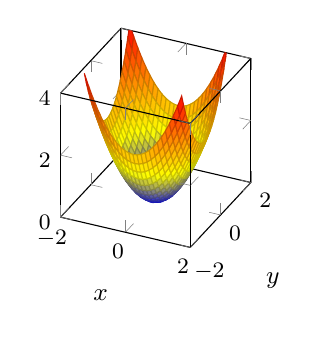
\begin{tikzpicture}
    \begin{axis}[
    xlabel=$x$, ylabel=$y$, small,
    xmin=-2, xmax=2,
    ymin=-2, ymax=2,
    zmin=0, zmax=4,
    3d box=complete,
    unit vector ratio*=1 1 1,
    ]
    \addplot3[surf, domain=-1.5:1.5] 
    {x^2+y^2};
    \end{axis}
    \end{tikzpicture} 

\item $Q(x, y) = -x^2 - y^2$, $Q < 0$.

    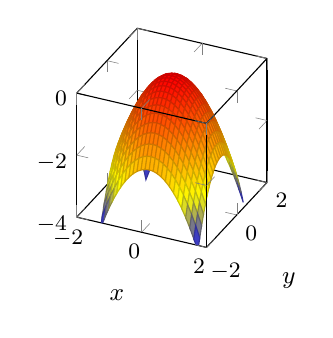
\begin{tikzpicture}
    \begin{axis}[
    xlabel=$x$, ylabel=$y$, small,
    xmin=-2, xmax=2,
    ymin=-2, ymax=2,
    zmin=-4, zmax=0,
    3d box=complete,
    unit vector ratio*=1 1 1,
    ]
    \addplot3[surf, domain=-1.5:1.5] 
    {-x^2-y^2};
    \end{axis}
    \end{tikzpicture} 

\item $Q(x, y) = x^2$, $Q \geq 0$.
    
    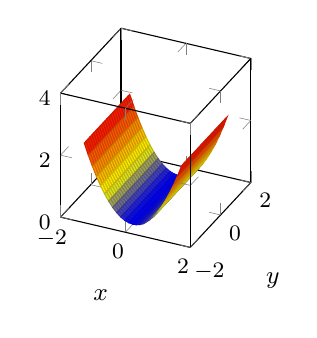
\begin{tikzpicture}
    \begin{axis}[
    xlabel=$x$, ylabel=$y$, small,
    xmin=-2, xmax=2,
    ymin=-2, ymax=2,
    zmin=0, zmax=4,
    3d box=complete,
    unit vector ratio*=1 1 1,
    ]
    \addplot3[surf, domain=-1.5:1.5] 
    {x^2};
    \end{axis}
    \end{tikzpicture} 

\item $Q(x, y) = -x^2$, $Q \leq 0$.

    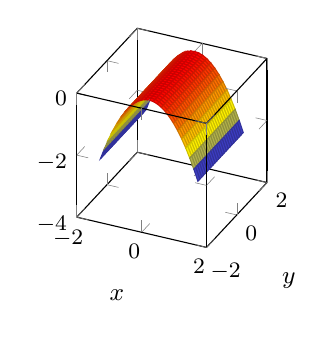
\begin{tikzpicture}
    \begin{axis}[
    xlabel=$x$, ylabel=$y$, small,
    xmin=-2, xmax=2,
    ymin=-2, ymax=2,
    zmin=-4, zmax=0,
    3d box=complete,
    unit vector ratio*=1 1 1,
    ]
    \addplot3[surf, domain=-1.5:1.5] 
    {-x^2};
    \end{axis}
    \end{tikzpicture} 

\item $Q(x, y) = x^2 - y^2$.

    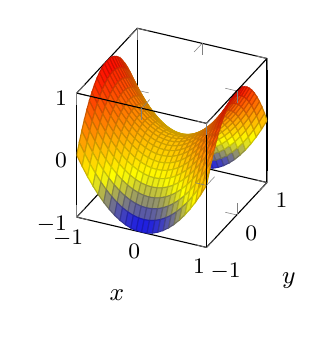
\begin{tikzpicture}
    \begin{axis}[
    xlabel=$x$, ylabel=$y$, small,
    xmin=-1, xmax=1,
    ymin=-1, ymax=1,
    zmin=-1, zmax=1,
    3d box=complete,
    unit vector ratio*=1 1 1,
    ]
    \addplot3[surf, domain=-1:1] 
    {x^2 - y^2};
    \end{axis}
    \end{tikzpicture} 

\end{enumerate}


\subsection{Одно применение квадратичных форм над $\RR$}

\href{https://www.dropbox.com/s/wwv38znnuts9rld/Qforms_application.pdf?dl=0}{Презентация} (продублирована ниже)

\subsubsection{Знаем из курса математического анализа}

Пусть $f\colon \RR \to \RR$ --- некоторая функция, $x_0 \in \RR$ --- некоторая точка.

Если $f$ дважды дифференцируема в точке $x_0$, то для малого приращения $y$ имеем
\begin{equation*}
    f(x_0 + y) = f(x_0) + ay + by^2 + o(y^2)
,\end{equation*}
где $a = f'(x_0)$, $b = f''(x_0) / 2$.

\begin{proposal}[необходимое условие локального экстремума]
    Если $f$ в точке $x_0$ имеет локальные экстремум, то $f'(x_0) = 0$.
\end{proposal}

\begin{proposal}[достаточные условия локального экстремума]
    Пусть $f'(x_0) = 0$. Тогда
    \begin{itemize}[nosep]
    \item если $f''(x_0) > 0$, то $f$ в точке $x_0$ имеет локальный минимум;
    \item если $f''(x_0) < 0$, то $f$ в точке $x_0$ имеет локальный максимум.
    \end{itemize}
\end{proposal}

\subsubsection{Применение квадратичных форм}

Пусть $f\colon \RR^n \to \RR$ --- некоторая функция, $x_0 \in \RR^n$ --- некоторая точка.

Если $f$ <<дважды дифференциируема>> в точке $x_0$, то для малого приращения $y = \begin{pmatrix} y_1 \\ \dots \\ y_n \end{pmatrix} \in \RR^n$ имеем

\begin{equation*}
    f(x_0 + y) = f(x_0) + \underbrace{a_1 y_1 + \dots + a_n y_n}_{l(y)} + \underbrace{\sum_{i = 1}^{n} b_{ii} y_i^2 + \sum_{1 \leq i < j \leq n} 2b_{ij} y_i y_j}_{Q(y)} + o(|y|^2)
.\end{equation*}

$l(y)$ --- линейная форма, (называется <<дифференциал>>)

$Q(y)$ --- квадратичная форма.

\begin{proposal}[необходимое условие локального экстремума]
    Если $f$ в точке $x_0$ имеет локальный экстремум, то $l(y) \equiv 0$ (то есть $a_1 = \dots = a_n = 0$).
\end{proposal}

\begin{proposal}[достаточные условие локального экстремума или его отсутствия]
    Пусть $l(y) \equiv 0$. Тогда:
    \begin{itemize}[nosep]
    \item если $Q > 0$, то $f$ в точке $x_0$ имеет локальный минимум;
    \item если $Q < 0$, то $f$ в точке $x_0$ имеет локальный максимум;
    \item если $Q$ неопределённа, то $f$ в точке $x_0$ не имеет локального экстремума.
    \end{itemize}
\end{proposal}

\subsection{Критерий Сильвестра положительной определённости квадратичной формы}

Пусть 
\begin{math}
    \begin{aligned}[t]
        &V \text{ --- векторное пространство над $\RR$, $\dim V = n$}, \\
        &\E = (e_1, \dots, e_n) \text{ --- базис $V$}, \\
        &B = B(Q, \E), \\
        &B_k \text{ --- левый верхний $k \times k$ блок}, \\
        &\delta_k = \det B_k.
    \end{aligned}
\end{math}

\begin{theorem}[Критерий Сильвестра положительной определенности]
    \begin{equation*}
        Q > 0 \iff \delta_k > 0 \ \forall k = 1 \dots n
    .\end{equation*}
\end{theorem}

\begin{proof}~
    \begin{description}
    \item[$\impliedby$] По следствию из метода Якоби, $i_+ = n$, то есть $Q > 0$.
    \item[$\implies$] $Q > 0 \implies \exists C \in M_n^0(\RR)$, такая что $C^TBC = E$.

        Тогда, $\det C^T \cdot \underset{= \delta_n}{\det B} \cdot \det C = 1$. Отсюда, $\delta_n = \frac{1}{(\det C)^2} > 0$.

        Теперь, для любого $k$ ограничение $Q$ на $\left< e_1, \dots, e_k \right>$ тоже положительно определённо, а его матрица в базисе $e_1, \dots, e_k$ равна $B_k$. Следовательно, $\det B_k > 0$.
        \qedhere
    \end{description}
\end{proof}

\subsection{Критерий отрицательной определённости квадратичной формы}

\begin{corollary}
    \begin{equation*}
        Q < 0 \iff \delta_k \begin{cases}
            > 0 & \text{при } k \divby 2, \\
            < 0 & \text{при } k \!\!\not\;\divby 2.
        \end{cases}
    \end{equation*}
\end{corollary}

\begin{proof}
    \begin{math}
        \begin{aligned}[t]
            Q < 0 &\iff -Q > 0 \\
                  &\iff \det (-B_k) > 0 \ \forall k \\
                  &\iff (-1)^{k} \delta_k > 0 \ \forall k
        \end{aligned}
    \end{math}
\end{proof}


\subsection{Евклидово пространство и скалярное произведение}

\begin{definition}
    \textit{Евклидово пространство} --- это векторное пространство $\EE$ над $\RR$, на котором задано \textit{скалярное произведение}, то есть такое отображение $(\bigcdot, \bigcdot)\colon \EE \times \EE \to \RR$, что
    \begin{enumerate}[nosep]
        \item $(\bigcdot, \bigcdot)$ --- симметричная билинейная форма,
        \item Квадратичная форма $(x, x)$ положительно определённая.
    \end{enumerate}
\end{definition}


\subsection{Примеры}

\begin{enumerate}
\item 
    $\EE = \RR^n$, $x = \begin{pmatrix} x_1 \\ \dots \\ x_n \end{pmatrix}$, $y = \begin{pmatrix} y_1 \\ \dots \\ y_n \end{pmatrix}$.

    $(x, y) := x_1 y_1 + \dots + x_n y_n \leftarrow $ стандартное скалярное произведение в $\RR^n$.

    $(x, x) = x_1^2 + \dots + x_n^2 > 0$.

\item
    $\EE = \text{Mat}_{m \times n}(\RR)$,

    $(A, B) := \tr (A^{T} B)$,

    $(A, A) = \tr (A^{T}A) = \sum_{i = 1}^{m} \sum_{j = 1}^{m} a_{ij}^2$.

\item
    $\EE = C[a, b]$,
    
    $(f, g) := \int_a^b f(x) g(x) \mathop{}\!dx$,

    $(f, f) = \int_a^b f^2(x) \mathop{}\!dx > 0$.
\end{enumerate}

    \section{Лекция 22}


\begin{comment}
    Всякое подпространство $U \subseteq E$ тоже является евклидовым пространством со скалярным произведением $(\bigcdot, \bigcdot) \big|_U \leftarrow$ ограничение на $U$.
\end{comment}


\subsection{Длина вектора евклидова пространства}

\begin{definition}
    \textit{Длина} вектора $x \in \EE$ --- это $|x| := \sqrt{(x, x)}$.
\end{definition}

\textbf{Свойства}:
    \begin{enumerate}[nosep] 
    \item $|x| \geq 0$, причем $|x| = 0 \iff x = 0$.
    \item $\lambda \in \RR \implies |\lambda \cdot x| = \underbrace{|\lambda|}_{\text{модуль}} \cdot \underbrace{|x|}_{\text{длина}} $
\end{enumerate}

\begin{example}
    Если $\EE = \RR^n$ со стандартным скалярным произведением, то $|x| = \sqrt{x_1^2 + \dots + x_n^2}$.
\end{example}

\begin{comment}
    Если $\EE = \text{Mat}_{m \times n}(\RR)$, $(A, B) = \tr(A^{T} B)$

    Тогда, $|A| = \sqrt{\sum_{i = 1}^{m} \sum_{j = 1}^{n} a_{ij}^2} \leftarrow$ это обозначается как $\norm{A}_{F}$ и называется \textit{нормой Фробениуса}, \textit{фробениусовой нормой}.
\end{comment}


\subsection{Неравенство Коши–Буняковского}

\begin{proposal}[неравенство Коши-Буняковского]
    $\forall x, y \in \EE$ верно $|(x, y)| \leq |x| \cdot |y|$, причём равенство $\iff$ $x$, $y$ пропорциональны.
\end{proposal}

\begin{proof}
    Случаи:
    \begin{enumerate}
    \item $x, y$ пропорциональны. Тогда, можно считать, что $y = \lambda x$, $\lambda \in \RR$.

        $|(x, y)| = |(x, \lambda x)| = |\lambda| |(x, x)| = |\lambda| |x|^2 = |x| \cdot |\lambda x| = |x| \cdot |y|$.

    \item $x, y$ не пропорциональны. Тогда $x, y$ линейно независимы.

        Значит они образуют базис в $\left< x, y \right>$.

        Получаем
        \begin{equation*}
            \begin{vmatrix} 
                (x, x) & (x, y) \\
                (y, x) & (y, y)
            \end{vmatrix} > 0 \quad \text{(критерий Сильвестра)}
        .\end{equation*}

        Отсюда, $(x, x) \cdot (y, y) - (x, y)^2 > 0 \implies (x, y)^2 < |x|^2 \cdot |y|^2$.
    \end{enumerate}
\end{proof}

\begin{example}
    Пусть $\EE = \RR^n$ со стандартным скалярным произведением, тогда
    \begin{equation*}
        |x_1 y_1 + \dots + x_n y_n| \leq \sqrt{x_1^2 + \dots + x_n^2} \cdot \sqrt{y_1^2 + \dots + y_n^2}
    .\end{equation*}
\end{example}


\subsection{Угол между ненулевыми векторами евклидова пространства}

Пусть $x, y \in \EE \setminus \{0\}$, тогда $-1 \leq \frac{(x, y)}{|x| \cdot |y|} \leq 1$.

\begin{definition}
    Угол между ненулевыми векторами $x, y \in \EE$, это такой $\alpha \in [0, \pi]$, что $\cos \alpha = \frac{(x, y)}{|x| \cdot |y|}$.

    Тогда $(x, y) = |x| |y| \cos \alpha$.
\end{definition}


\subsection{Матрица Грама системы векторов евклидова пространства}

Пусть $v_1, \dots, v_k$ --- произвольная система векторов.

\begin{definition}
    \textit{Матрица Грама} этой системы --- это
    \begin{equation*}
        G(v_1, \dots, v_k) = \begin{pmatrix}
            (v_1, v_1) & (v_1, v_2) & \dots & (v_1, v_k) \\
            (v_2, v_1) & (v_2, v_2) & \dots & (v_2, v_k) \\
            \vdots & \vdots & \ddots & \vdots \\
            (v_k, v_1) & (v_k, v_2) & \dots & (v_k, v_k)
        \end{pmatrix}
    .\end{equation*}
\end{definition}

\begin{example}
    $\EE = \RR^n$ со стандартным скалярным произведением.

    $a_1, \dots, a_k \in \RR^n \leadsto A := (a_1, \dots, a_k) \in \text{Mat}_{n \times k}(\RR)$.

    Тогда, $G(a_1, \dots, a_k) = A^T \cdot A$.
\end{example}


\subsection{Определитель матрицы Грама: неотрицательность, критерий положительности}

\begin{proposal}
    $\forall v_1, \dots, v_k \in \EE \implies \det G(v_1, \dots, v_k) \geq 0$.

    Более того, $\det G(v_1, \dots, v_k) > 0 \iff v_1, \dots, v_k$ линейно независимы. 
\end{proposal}

\begin{proof}
    Пусть $G := G(v_1, \dots, v_k)$.
    Случаи:
    \begin{enumerate}
    \item $v_1, \dots, v_k$ линейно независимы. Тогда, $G$ --- матрица билинейной формы $(\bigcdot, \bigcdot) \Big|_{\left< v_1, \dots, v_k \right>}$ в базисе $v_1, \dots, v_k$ подпространства $\left< v_1, \dots, v_k \right>$, а значит $\det G > 0$ по критерию Сильвестра.
    
    \item $v_1, \dots, v_k$ линейно зависимы. Тогда, $\exists (\alpha_1, \dots, \alpha_k) \in \RR^k \setminus \{0\}$, такие что $\alpha_1 v_1 + \dots + \alpha_k v_k = 0$.

        А значит,  $\forall i = 1, \dots, k \implies \alpha_1 (v_1, v_i) + \dots + \alpha_k (v_k, v_i) = 0$.
        
        Отсюда, $a_1 G_{(1)} + \dots + \alpha_k G_{(k)} = 0 \implies$ строки в $G$ линейно зависимы $\implies \det G = 0$.
        \qedhere
    \end{enumerate}
\end{proof}


\subsection{Ортогональные векторы}

\begin{definition}
    Векторы $x, y \in \EE$ называются \textit{ортогональными}, если $(x, y) = 0$.
\end{definition}


\subsection{Ортогональное дополнение подмножества евклидова пространства}

\begin{definition}
    \textit{Ортогональное дополнение} множества $S \subseteq \EE$ --- это множество $S^{\perp} := \{x \in \EE \mid (x, y) = 0 \ \forall y \in S\}$.
\end{definition}

\begin{exercise}~
    \begin{enumerate}
    \item $S^{\perp}$ --- подпространство в $\EE$.
    \item $S^{\perp} = \left< S \right>^{\perp}$.
    \end{enumerate}
\end{exercise}

\subsection{Размерность ортогонального дополнения подпространства, ортогональное дополнение к ортогональному дополнению подпространства}
\subsection{Разложение евклидова пространства в прямую сумму подпространства и его ортогонального дополнения}

Далее считаем, что $\dim \EE = n < \infty$.

\begin{proposal}
    Пусть $S \subseteq \EE$ --- подпространство.
    Тогда:
    \begin{enumerate}
    \item $\dim S^{\perp} = n - \dim S$.
    \item $\EE = S \oplus S^{\perp}$.
    \item $(S^{\perp})^{\perp} = S$.
    \end{enumerate}
\end{proposal}

\begin{proof}~
    \begin{enumerate}
    \item 
        Пусть $\dim S = k$ и $e_1, \dots, e_k$ --- базис $S$.
        
        Дополним $e_1, \dots, e_k$ до базиса $e_1, \dots, e_n$ всего $\EE$.

        Тогда, $\forall x = x_1 e_1 + \dots + x_n e_n \in \EE$.

        \begin{align*}
            x \in S^{\perp} &\iff (x, e_i) = 0 \ \forall i = 1, \dots, k \\
                            &\iff \begin{cases}
                                (e_1, e_1) x_1 + \dots + (e_n, e_1) x_n = 0 \\
                                (e_1, e_2) x_1 + \dots + (e_n, e_2) x_n = 0 \\
                                \dots \\
                                (e_1, e_k) x_1 + \dots + (e_n, e_k) x_n = 0
                            \end{cases}
        .\end{align*}

        Это ОСЛУ с матрицей $G \in \text{Mat}_{k \times n}(\RR)$, причём левый $k \times k$ блок в $G$ --- это $\underbrace{G(e_1, \dots, e_k)}_{\det \neq 0}$.

        Это означает, что $\rk G = k$.

        Следовательно, пространство решений этой ОСЛУ имеет размерность $n - k$.

        Отсюда, $\dim S^{\perp} = n - k = n - \dim S$.

    \item
        \begin{enumerate}
        \item $\dim S + \dim S^{\perp} = k + (n - k) = n = \dim E$.
        \item $v \in S \cap S^{\perp} \implies (v, v) = 0 \implies v = 0 \implies S \cap S^{\perp} = \{0\}$.
        \end{enumerate}

        А значит, $E = S \oplus S^{\perp}$.

    \item
        Заметим, что $S \subseteq (S^{\perp})^{\perp}$ (по определению).

        $\dim (S^{\perp})^{\perp} = n - \dim S^{\perp} = n - (n - \dim S) = \dim S$.

        Следовательно, $S = (S^{\perp})^{\perp}$.
        \qedhere
    \end{enumerate}
\end{proof}


\subsection{Ортогональная проекция вектора на подпространство, ортогональная составляющая вектора относительно подпространства}

$S$ --- подпространство $ \implies \EE = S \oplus S^{\perp}$

$\forall v \in \EE \ \exists! \ x \in S, y \in S^{\perp}$, такие что $x + y = v$.

\begin{definition}~
    \begin{enumerate}
    \item 
        $x$ называется \textit{ортогональной проекцией} вектора $v$ на подпространство $S$.

        Обозначение: $x = \pr_S v$.

    \item
        $y$ называется \textit{ортогональной составляющей} вектора $v$ относительно подпространства $S$.

        Обозначение: $y = \ort_S v$.
    \end{enumerate}
\end{definition}

\subsection{Явная формула для ортогональной проекции вектора на подпространство в $\RR^n$, заданное своим базисом}

Пусть $\EE = \RR^n$ со стандартным скалярным произведением.

$S \subseteq \EE$ --- подпространство, $a_1, \dots, a_k$ --- базис $S$.

Пусть $A := (a_1, \dots, a_k) \in \text{Mat}_{n \times k}(\RR)$, $A^{(i)} = a_i$.

\begin{proposal}
    $\forall v \in \RR^n \quad \pr_S v = A (A^{T} A)^{-1} A^{T} v$.
\end{proposal}

\begin{proof}
    Корректность: $A^{T} A = G(a_1, \dots, a_k) \in M_k^{0}(\RR)$.

    Положим $x := \pr_S v$, $y := \ort_S v$.

    Так как $x \in S$, $x = A \cdot \begin{pmatrix} \alpha_1 \\ \dots \\ \alpha_k \end{pmatrix}$, $\alpha_i \in \RR$.

    $y \in S^{\perp} \implies A^T y = 0$.

    \begin{align*}
    A (A^{T} A)^{-1} A^{T} v
    &= A(A^{T}A)^{-1}A^{T} (x + y) \\
    &= A\lefteqn{\underbracket{\phantom{(A^{T}A)^{-1}A^{T} A}}_E} (A^{T} A)^{-1} A^{T} \overbracket{A \begin{pmatrix} \alpha_1 \\ \dots \\ \alpha_k \end{pmatrix}}^{x} + A(A^{T} A)^{-1} \underbracket{A^{T} y}_{0} \\
    &= A \begin{pmatrix} \alpha_1 \\ \dots \\ \alpha_k \end{pmatrix} = x = \pr_S v
    .\end{align*}
\end{proof}


\subsection{Ортогональные и ортонормированные системы векторов}

\begin{definition}
    Система ненулевых векторов $v_1, \dots, v_k$ называется
    \begin{enumerate}[nosep]
        \item \textit{ортогональной}, если $(v_i, v_j) = 0 \ \forall i \neq j$ (то есть $G(v_1, \dots, v_k)$ диагональна),
        \item \textit{ортонормированной}, если $(v_i, v_j) = 0 \ \forall i \neq j$ и $(v_i, v_i) = 1$ ($\iff |v_i| = 1$).
            То есть $G(v_1, \dots, v_k) = E$.
    \end{enumerate}
\end{definition}

\begin{comment}
    Всякая ортогональная (и в частности ортонормированная) система векторов автоматически линейно независима.
    \begin{equation*}
        \det G(v_1, \dots, v_k) = |v_1|^2 \cdot |v_2|^2 \dotsm |v_k|^2 \neq 0
    .\end{equation*}
\end{comment}


\subsection{Ортогональный и ортонормированный базис}

\begin{definition}
    Базис пространства называется \textit{ортогональным} (соответственно \textit{ортонормированным}), если он является ортогональной (ортонормированной) системой векторов.
\end{definition}

    \section{Лекция 05.03.2020}


\subsection{Описание всех ортонормированных базисов в терминах одного ортонормированного базиса и матриц перехода}

Пусть $\E = (e_1, \dots, e_n)$ --- ортонормированный базис в $E$.

Пусть $\E' = (e'_1, \dots, e'_n)$ --- какой-то другой базис.

$(e'_1, \dots, e'_n) = (e_1, \dots, e_n) \cdot C$, $C \in M_n^{0}(\RR)$.

\begin{proposal}
    $\E'$ --- ортонормированный базис $\iff C^{T} \cdot C = E$.
\end{proposal}

\begin{proof}
    $G(e'_1, \dots, e'_n) = C^{T} \underbracket{G(e_1, \dots, e_n)}_E C = C^{T} C$.

    $\E'$ ортонормированный $\iff G(e'_1, \dots, e'_n) = E \iff C^{T} C = E$.
\end{proof}


\subsection{Ортогональные матрицы и их свойства}

\begin{definition}
    Матрица $C \in M_n(\RR)$ называется \textit{ортогональной} если $C^{T} C = E$.
\end{definition}

\begin{comment}
    $C^{T} C = E \iff C C^{T} = E \iff C^{-1} = C^{T}$.
\end{comment}

\begin{properties}~
    \begin{enumerate}
    \item $C^{T} C = E \implies $ система столбцов $C^{(1)}, \dots, C^{(n)}$ --- это ортонормированный базис в $\RR^n$,
    \item $C C^{T} = E \implies $ система строк $C_{(1)}, \dots, C_{(n)}$ --- это тоже ортонормированный базис в $\RR^n$,
    \end{enumerate}
    В частности, $|c_{ij}| \leq 1$.
    \begin{enumerate}[resume]
    \item $\det C = \pm 1$.
    \end{enumerate}
\end{properties}

\begin{example}
    $n = 2$.
    Ортогональный матрицы:
    \begin{equation}
        \begin{gathered}
            \begin{pmatrix} 
                \cos \phi & -\sin \phi \\
                \sin \phi & \cos \phi
            \end{pmatrix} \\
            \det = 1
        \end{gathered}
        \hspace{1cm}
        \begin{gathered}
            \begin{pmatrix} 
                \cos \phi & \sin \phi \\
                \sin \phi & -\cos \phi
            \end{pmatrix} \\
            \det = -1
        \end{gathered}
    .\end{equation}
\end{example}


\subsection{Ортогональное дополнение подмножества евклидова пространства}

\begin{definition}
    \textit{Ортогональное дополнение} множества $S \subseteq \EE$ --- это множество $S^{\perp} := \{x \in \EE \mid (x, y) = 0 \ \forall y \in S\}$.
\end{definition}

\begin{exercise}~
    \begin{enumerate}
    \item $S^{\perp}$ --- подпространство в $\EE$.
    \item $S^{\perp} = \left< S \right>^{\perp}$.
    \end{enumerate}
\end{exercise}


\subsection{Размерность ортогонального дополнения подпространства, ортогональное дополнение к ортогональному дополнению подпространства}
\subsection{Разложение евклидова пространства в прямую сумму подпространства и его ортогонального дополнения}

Далее считаем, что $\dim \EE = n < \infty$.

\begin{proposal}
    Пусть $S \subseteq \EE$ --- подпространство.
    Тогда:
    \begin{enumerate}
    \item $\dim S^{\perp} = n - \dim S$.
    \item $\EE = S \oplus S^{\perp}$.
    \item $(S^{\perp})^{\perp} = S$.
    \end{enumerate}
\end{proposal}

\begin{proof}~
    \begin{enumerate}
    \item 
        Пусть $\dim S = k$ и $e_1, \dots, e_k$ --- базис $S$.
        
        Дополним $e_1, \dots, e_k$ до базиса $e_1, \dots, e_n$ всего $\EE$.

        Тогда, $\forall x = x_1 e_1 + \dots + x_n e_n \in \EE$.

        \begin{align*}
            x \in S^{\perp} &\iff (x, e_i) = 0 \ \forall i = 1, \dots, k \\
                            &\iff \begin{cases}
                                (e_1, e_1) x_1 + \dots + (e_n, e_1) x_n = 0 \\
                                (e_1, e_2) x_1 + \dots + (e_n, e_2) x_n = 0 \\
                                \dots \\
                                (e_1, e_k) x_1 + \dots + (e_n, e_k) x_n = 0
                            \end{cases}
        .\end{align*}

        Это ОСЛУ с матрицей $G \in \text{Mat}_{k \times n}(\RR)$, причём левый $k \times k$ блок в $G$ --- это $\underbrace{G(e_1, \dots, e_k)}_{\det \neq 0}$.

        Это означает, что $\rk G = k$.

        Следовательно, пространство решений этой ОСЛУ имеет размерность $n - k$.

        Отсюда, $\dim S^{\perp} = n - k = n - \dim S$.

    \item
        \begin{enumerate}
        \item $\dim S + \dim S^{\perp} = k + (n - k) = n = \dim E$.
        \item $v \in S \cap S^{\perp} \implies (v, v) = 0 \implies v = 0 \implies S \cap S^{\perp} = \{0\}$.
        \end{enumerate}

        А значит, $E = S \oplus S^{\perp}$.

    \item
        Заметим, что $S \subseteq (S^{\perp})^{\perp}$ (по определению).

        $\dim (S^{\perp})^{\perp} = n - \dim S^{\perp} = n - (n - \dim S) = \dim S$.

        Следовательно, $S = (S^{\perp})^{\perp}$.
        \qedhere
    \end{enumerate}
\end{proof}


\subsection{Ортогональная проекция вектора на подпространство, ортогональная составляющая вектора относительно подпространства}

$S$ --- подпространство $ \implies \EE = S \oplus S^{\perp}$

$\forall v \in \EE \ \exists! \ x \in S, y \in S^{\perp}$, такие что $x + y = v$.

\begin{definition}~
    \begin{enumerate}
    \item 
        $x$ называется \textit{ортогональной проекцией} вектора $v$ на подпространство $S$.

        Обозначение: $x = \pr_S v$.

    \item
        $y$ называется \textit{ортогональной составляющей} вектора $v$ относительно подпространства $S$.

        Обозначение: $y = \ort_S v$.
    \end{enumerate}
\end{definition}


\subsection{Формула для ортогональной проекции вектора на подпространство в терминах его ортогонального (ортонормированного) базиса}


Пусть $S \subseteq \EE$ --- подпространство.

$e_1, \dots, e_k$ --- ортогональный базис в $S$.

\begin{proposal}
    $\forall v \in \EE \quad \pr_S v = \sum_{i = 1}^{k} \dfrac{(v, e_i)}{(e_i, e_i)} e_i$.

    В частности, если $e_1, \dots, e_k$ ортонормирован, то $\pr_S v = \sum_{i = 1}^{k} (v, e_i) e_i$.
\end{proposal}

\begin{proof}
    Пусть $e_{k + 1}, \dots, e_n$ --- ортогональный базис в $S^{\perp}$. Тогда $e_1, \dots, e_n$ --- ортогональный базис в $\EE$.

    \begin{equation*}
        v = \underbrace{\sum_{i = 1}^{k} \dfrac{(v, e_i)}{(e_i, e_i)} e_i}_{\in S} + \underbrace{\sum_{i = k + 1}^{n} \dfrac{(v, e_i)}{(e_i, e_i)} e_i}_{\in S^{\perp}}
    .\end{equation*}

    Отсюда,
    \begin{equation*}
        \pr_S v = \sum_{i = 1}^{k} \dfrac{(v, e_i)}{(e_i, e_i)}
    .\qedhere\end{equation*}
\end{proof}


\begin{comment}
    \hyperref[lec22:gram-schmidt_second_property]{Свойство 2} из метода Грама-Шмидта говорит, что 
    \begin{equation*}
        f_i = e_i - \pr_{\left< f_1, \dots, f_{i - 1}\right>} e_i = \ort_{\left< f_1, \dots, f_{i - 1} \right>} e_i
    .\end{equation*}
\end{comment}


\subsection{Явная формула для ортогональной проекции вектора на подпространство в $\RR^n$, заданное своим базисом}

Пусть $\EE = \RR^n$ со стандартным скалярным произведением.

$S \subseteq \EE$ --- подпространство, $a_1, \dots, a_k$ --- базис $S$.

Пусть $A := (a_1, \dots, a_k) \in \text{Mat}_{n \times k}(\RR)$, $A^{(i)} = a_i$.

\begin{proposal}
    $\forall v \in \RR^n \quad \pr_S v = A (A^{T} A)^{-1} A^{T} v$.
\end{proposal}

\begin{proof}
    Корректность: $A^{T} A = G(a_1, \dots, a_k) \in M_k^{0}(\RR)$.

    Положим $x := \pr_S v$, $y := \ort_S v$.

    Так как $x \in S$, $x = A \cdot \begin{pmatrix} \alpha_1 \\ \dots \\ \alpha_k \end{pmatrix}$, $\alpha_i \in \RR$.

    $y \in S^{\perp} \implies A^T y = 0$.

    \begin{align*}
    A (A^{T} A)^{-1} A^{T} v
    &= A(A^{T}A)^{-1}A^{T} (x + y) \\
    &= A\lefteqn{\underbracket{\phantom{(A^{T}A)^{-1}A^{T} A}}_E} (A^{T} A)^{-1} A^{T} \overbracket{A \begin{pmatrix} \alpha_1 \\ \dots \\ \alpha_k \end{pmatrix}}^{x} + A(A^{T} A)^{-1} \underbracket{A^{T} y}_{0} \\
    &= A \begin{pmatrix} \alpha_1 \\ \dots \\ \alpha_k \end{pmatrix} = x = \pr_S v
    .\end{align*}
\end{proof}


\subsection{Теорема Пифагора в евклидовом пространстве}

\begin{theorem}
    Пусть $x, y \in \EE$, $(x, y) = 0$. Тогда $|x + y|^2 = |x|^2 + |y|^2$.
\end{theorem}

\begin{proof}
    \begin{equation*}
        |x + y|^2 = (x + y, x + y) = \underbrace{(x, x)}_{|x|^2} + \underbrace{(x, y)}_{0} + \underbrace{(y, x)}_{0} + \underbrace{(y, y)}_{|y|^2} = |x|^2 + |y|^2
    .\qedhere\end{equation*}
\end{proof}


\subsection{Расстояние между векторами евклидова пространства}

\begin{definition}
    \textit{Расстояние} между векторами $x, y \in \EE$ --- это $\rho(x, y) = |x - y|$.
\end{definition}


\subsection{Неравенство треугольника}

\begin{proposal}
    $\forall a, b, c \in \EE \implies \rho(a, b) + \rho(b, c) \geq \rho(a, c)$.
\end{proposal}

\begin{proof}
    Пусть $x = a - b$, $y = b - c$. Тогда, $a - c = x + y$.
    Достаточно доказать, что $|x| + |y| \geq |x + y|$.

    \begin{equation*}
        |x + y|^2 = |x|^2 + \underbrace{2(x, y)}_{\leq |x||y|} + |y|^2 \leq |x|^2 + 2|x||y| + |y|^2 = (|x| + |y|)^2
    .\qedhere\end{equation*}
\end{proof}


\subsection{Расстояние между двумя подмножествами евклидова пространства}

Пусть $P, Q \subseteq \EE$ --- два подмножества.

\begin{definition}
    \textit{Расстояние} между $P$ и $Q$ --- это
    \begin{equation*}
        \rho(P, Q) := \inf_{x \in P, y \in Q} \rho(x, y)
    .\end{equation*}
\end{definition}


\subsection{Теорема о расстоянии от вектора до подпространства}

\begin{theorem}
    Пусть $x \in \EE$, $S \subseteq \EE$ --- подпространство. Тогда, $\rho(x, S) = \left|\ort_S x\right|$, причем $\pr_S x$ --- это ближайший к $x$ вектор из $S$.
\end{theorem}

\begin{proof}
    Положим $y = \pr_S x$, $z = \ort_S x$. Тогда, $x = y + z$.
    Для любого $y' \in S$, $y' \neq 0$ имеем
    \begin{equation*}
        \rho(x, y + y')^2 = |x - y - y'|^2 = |z - y'|^2 = |z|^2 + |y'|^2 > |z|^2 = |x - y|^2 = \rho(x, y)^2
    .\qedhere\end{equation*}
\end{proof}


\subsection{Псевдорешение несовместной системы линейных уравнений (метод наименьших квадратов)}

СЛУ $Ax = b$, $A \in \text{Mat}_{m \times n}(\RR)$, $x \in \RR^n$, $b \in \RR^m$.
\begin{equation*}
    x_0 \text{ --- решение системы} \iff Ax_0 = b \iff Ax_0 - b = 0 \iff |Ax_0 - b| = 0 \iff \rho(Ax_0, b) = 0
.\end{equation*}

Если СЛУ несовместна, то $x_0$ называется \textit{псевдорешением}, если $\rho(Ax_0, b)$ минимально.

\begin{equation*}
    \rho(Ax_0, b) = \min_{x \in R^n} \rho(Ax, b)
.\end{equation*}

$x_0$ --- решение задачи оптимизации $\rho(Ax, b) \xrightarrow[x \in \RR^n]{} \min$.

    \section{Лекция 24} 

\subsection{Метод наименьших квадратов для несовместных систем линейных уравнений: постановка задачи и её решение}

Пусть $S \subseteq \RR^n$ --- подпространство натянутое на столбцы матрицы $A$.

$S = \left< A^{(1)}, \dots, A^{(n)} \right>$.

Положим $c := \pr_S b$.

\begin{proposal}~
    \begin{enumerate}
    \item $x_0$ --- псевдорешение $Ax = b \iff x_0$ --- решение для $Ax = c$.  
    \item Если столбцы $A^{(1)}, \dots, A^{(n)}$ линейно независимы, то псевдорешение единственно и может быть найдено по формуле $x_0 = (A^{T} A)^{-1} A^{T} b$.
    \end{enumerate}
\end{proposal}


\subsection{Единственность псевдорешения и явная формула для него в случае линейной независимости столбцов матрицы коэффициентов}

\begin{proof}~
    \begin{enumerate}
        \item
            \begin{equation*}
                \forall x \in \RR^n \quad Ax = x_1 A^{(1)} + \dots + x_n A^{(n)} \implies \{Ax \mid x \in \RR^n\} = S \implies \min_{x \in \RR^n} \rho(Ax, b) = \rho(S, b)
            .\end{equation*}
            По теореме о расстоянии от вектора до подпространства минимум достигается при $Ax = c = \pr_S b$.

        \item
            Так как $A^{(1)}, \dots, A^{(n)}$ линейно независимы, то $c$ единственным образом представим в виде линейной комбинации этих столбцов.

            Следовательно, $x_0$ единственно.

            Знаем, что $A \underbrace{(A^{T} A)^{-1} A^{T} b} = c$. Значит, $x_0 = (A^{T} A)^{-1} A^{T} b$.
            \qedhere
    \end{enumerate}
\end{proof}

\begin{example}
    \begin{math}
        \begin{cases}
            x = 0, \\
            x = 1.
        \end{cases}
    \end{math}

    Здесь $A = \begin{pmatrix} 1 \\ 1 \end{pmatrix}$, $b = \begin{pmatrix} 0 \\ 1 \end{pmatrix}$.

    Тогда, $x_0 = \left[\begin{pmatrix} 1 & 1 \end{pmatrix}\begin{pmatrix} 1 \\ 1 \end{pmatrix}\right]^{-1} \begin{pmatrix} 1 & 1 \end{pmatrix}\begin{pmatrix} 0 \\ 1 \end{pmatrix} = \frac{1}{2}$.
    
    \bigskip
    {\tiny Здесь должна была быть картинка, но мне лень. Пинать можно @darkkeks.}
\end{example}


\subsection{Формула для расстояния от вектора до подпространства в терминах матриц Грама}

Пусть $\EE$ --- евклидово пространство, $\dim \EE = n < \infty$.

$S \subseteq \EE$ --- подпространство, $e_1, \dots, e_k$ --- базис в $S$.

\begin{theorem}
    $\forall x \in \EE \quad \rho(x, S)^2 = \dfrac{\det G(e_1, \dots, e_k, x)}{\det G(e_1, \dots, e_k)}$.
\end{theorem}

\begin{proof}
    Пусть $z := \ort_S x$, тогда $\rho(x, S)^2 = |z|^2$.

    \begin{enumerate}
    \item $x \in S \implies \rho(x, S) = 0$:

        так как $e_1, \dots, e_k, x$ --- линейно зависимы, то $\det G(e_1, \dots, e_k, x) = 0$.

    \item $x \not\in S$.

        Ортогонализация Грама-Шмидта: $e_1, \dots, e_k, x \leadsto f_1, \dots, f_k, z$.

        По свойству \ref{lec22:heart} получаем
        \begin{equation*}
            \dfrac{\det G(e_1, \dots, e_k, x)}{\det G(e_1, \dots, e_k)} = \dfrac{\det G(f_1, \dots, f_k, z)}{\det G(f_1, \dots, f_k)} = \frac{|f_1|^2 \dots |f_k|^2 |z|^2}{|f_1|^2 \dots |f_k|^2} = |z|^2 = \rho(x, S)^2
        .\end{equation*}
    \end{enumerate}
\end{proof}


\subsection{$k$-мерный параллелепипед}

\begin{definition}
    \textit{$k$-мерный параллелепипед}, натянутый на векторы $a_1, \dots, a_k$, это множество
    \begin{equation*}
        P(a_1, \dots, a_k) := \left\{ \sum_{i = 1}^{k} x_i a_i \mid 0 \leq x_i < 1 \right\}
    .\end{equation*}

    Основание: $P(a_1, \dots, a_{k - 1})$.

    Высота: $h := \ort_{\left< a_1, \dots, a_{k - 1} \right>} a_k$.
\end{definition}

\begin{example}~
    {\tiny если у кого-то есть фото с доски в хорошем качестве или, что лучше, рисунок этого, напишите @nih3kwo}
    \begin{description}
    \item[$k = 1 \colon$] \  $P(a_1)$ --- отрезок.
    \item[$k = 2 \colon$] \ $P(a_1, a_2)$ --- параллелограмм. \  Основание --- $P(a_1)$, высота --- $|h|$.
    \item[$k = 3 \colon$] \ $P(a_1, a_2, a_3)$ --- классический параллелепипед. \ Основние --- $P(a_1, a_2)$, высотка --- $|h|$. 
    \end{description}
\end{example}


\subsection{Объём $k$-мерного параллелепипеда в евклидовом пространстве}

\begin{definition}
    \textit{$k$-мерный объем} $k$-мерного параллелепипеда $P(a_1, \dots, a_k)$ --- это величина $\vol P(a_1, \dots, a_k)$, определяемая индуктивно:

    \begin{description}
    \item[$k = 1$] $\implies \vol P(a_1) := |a_1|$.
    \item[$k > 1$] $\implies \vol P(a_1, \dots, a_k) := \vol P(a_1, \dots, a_{k - 1}) \cdot |h|$.
    \end{description}
\end{definition}


\subsection{Вычисление объёма $k$-мерного параллелепипеда при помощи определителя матрицы Грама задающих его векторов}

\begin{theorem}
    $\vol P(a_1, \dots, a_k)^2 = \det G(a_1, \dots, a_k)$.
\end{theorem}

\begin{proof}
    Индукция по $k$:

    \begin{description}
    \item[$k = 1:$] $|a_1|^2 = (a_1, a_1)$ --- верно.
    \item[$k > 1:$] $\vol P(a_1, \dots, a_k)^2 = \vol P(a_1, \dots, a_{k - 1})^2 \cdot |h|^2 = \det G(a_1, \dots, a_{k - 1}) \cdot |h|^2 = (\star)$.

        Если $a_1, \dots, a_{k - 1}$ линейно независимы, то $|h|^2 = \dfrac{\det G(a_1, \dots, a_k)}{\det G(a_1, \dots, a_{k - 1})}$.
        Тогда, $(\star) = \det G(a_1, \dots, a_k)$.

        Если же $a_1, \dots, a_{k - 1}$ линейно зависимы, то $\det G(a_1, \dots, a_{k - 1}) = 0 \implies (\star) = 0$. Но $a_1, \dots, a_k$ тоже линейно зависимы, а значит $\det G(a_1, \dots, a_k) = 0$.
        \qedhere
    \end{description}
\end{proof}

\begin{corollary}
    $\vol P(a_1, \dots, a_k)$ не зависит от выбора основания.
\end{corollary}

\begin{example}
    Пусть $a_1, \dots, a_k$ ортогональны, тогда $P(a_1, \dots, a_k)$ --- <<прямоугольный параллелепипед>>.

    \begin{equation*}
        \vol P(a_1, \dots, a_k) = \sqrt{\det G(a_1, \dots, a_k)} = \sqrt{|a_1|^2 \dots |a_k|^2} = |a_1| \dots |a_k|
    .\end{equation*}
\end{example}


\subsection{Формула для объёма $n$-мерного параллелепипеда в $n$-мерном евклидовом пространстве в терминах координат задающих его векторов в ортонормированном базисе}

Пусть $(e_1, \dots, e_n)$ --- ортонормированный базис в $\EE$,

$(a_1, \dots, a_n) = (e_1, \dots, e_n) \cdot A$, $A \in M_n(\RR)$.

\begin{proposal}
    $\vol P(a_1, \dots, a_n) = \left|\det A\right|$.
\end{proposal}

\begin{proof}
    \begin{equation*}
        G(a_1, \dots, a_n) = A^{T} \cdot A \implies \vol P(a_1, \dots, a_n) = \sqrt{\det (A^{T} A)} = \sqrt{\left(\det A\right)^2} = |\det A|
        \qedhere
    .\end{equation*}
\end{proof}


\subsection{Отношение одинаковой ориентированности на множестве базисов евклидова пространства}

Пусть $\E = (e_1, \dots, e_n)$ и $\E' = (e'_1, \dots, e'_n)$ --- два базиса в $\EE$.

$(e'_1, \dots, e'_n) = (e_1, \dots, e_n) \cdot C$, $C \in M_n^0(\RR)$.

\begin{definition}
    Говорят, что $\E$ и $\E'$ одинаково ориентированы, если $\det C > 0$.
\end{definition}

\begin{exercise}~
    \begin{enumerate}
    \item 
        Отношение одинаковой ориентированности является отношением эквивалентности на множестве всех базисов~в~$\EE$.
    \item 
        Имеется ровно 2 класса эквивалентности.
    \end{enumerate}
\end{exercise}


\subsection{Ориентация в евклидовом пространстве}

\begin{definition}
    Говорят, что в $\EE$ задана ориентация, если все базисы одного класса объявлены положительно ориентированными, а все базисы другого класса объявлены отрицательно ориентированными.
\end{definition}

\begin{example}
    Стандартный выбор ориентации в $\RR^3$:

    Положительно ориентированные: <<правые>> тройки.

    Отрицательно ориентированные: <<левые>> тройки.

    \bigskip
    Тут показывать надо, но попробую описать словами: берем правую руку, и нумеруем пальцы начиная с большого (большой --- первый вектор, указательный --- второй, средний --- третий). Такую тройку векторов назовём <<правой>>. Аналогично можно сделать для левой руки. Суть в том, что никакую правую тройку векторов невозможно перевести в левую непрерывным преобразованием (так чтобы в процессе тройка оставалось базисом).
\end{example}


\subsection{Ориентированный объём n-мерного параллелепипеда в $n$-мерном евклидовом пространстве}

Фиксируем ориентацию в $\EE$.

Фиксируем положительно ориентированный ортонормированный базис $\E = (e_1, \dots, e_n)$ в $\EE$.

Пусть $a_1, \dots, a_n \in \EE$, $(a_1, \dots, a_n) = (e_1, \dots, e_n) \cdot A$.

\begin{definition}
    \textit{Ориентированным объемом} параллелепипеда $P(a_1, \dots, a_n)$ называется величина
    \begin{equation*}
        \Vol (a_1, \dots, a_n) = \det A
    .\end{equation*}
\end{definition}

\begin{proposal}
    $\Vol P(a_1, \dots, a_n)$ определён корректно, то есть не зависит от выбора положительно ориентированного ортонормированного базиса в $\EE$.
\end{proposal}

\begin{proof}
    Пусть $\E'$ --- другой положительно ориентированный ортонормированный базис, тогда $\E' = \E C$, где $C$ --- ортогональная матрица.
    В частности, $\det C = \pm 1$.
    Так как $\E$ и $\E'$ одинаково ориентированны, то $\det C = 1$.
    Тогда,
    \begin{equation*}
        (a_1, \dots, a_n) = (e'_1, \dots, e'_n) \cdot C^{-1} \cdot A \implies \Vol(a_1, \dots, a_n)_\text{новый} = \det \left(C^{-1} A\right) = \det A = \Vol (a_1, \dots, a_n)_\text{старый}
    .\qedhere\end{equation*}
\end{proof}

Свойства ориентированного объема:
\begin{enumerate}[nosep]
\item $\Vol(a_1, \dots, a_n)$ линеен по каждому аргументу.
\item $\Vol(a_1, \dots, a_n)$ кососимметрична (то есть меняет знак при перестановке любых двух аргументов).
\item $\Vol(a_1, \dots, a_n) > 0 \iff (a_1, \dots, a_n)$ --- положительно ориентированный базис в $\EE$.
\item $\Vol(a_1, \dots, a_n) < 0 \iff (a_1, \dots, a_n)$ --- отрицательно ориентированный базис в $\EE$.
\item $\Vol(a_1, \dots, a_n) = 0 \iff (a_1, \dots, a_n)$ линейно зависимы.
\end{enumerate}

    \section{Лекция 25} 

\href{https://www.dropbox.com/s/y3r4x7mjt7iv71a/%D0%9B%D0%90%D0%B8%D0%93_19-20_%D0%9B%D0%B5%D0%BA%D1%86%D0%B8%D1%8F_25.pdf?dl=0}{Записки с лекции}


\begin{lemma}
    Пусть $v_1, v_2 \in \EE$. Тогда, $(v_1, x) = (v_2, x) \ \forall x \in \EE \implies v_1 = v_2$.
\end{lemma}

\begin{proof}
    Имеем $(v_1 - v_2, x) = 0 \ \forall x \in \EE$.
    Тогда, $v_1 - v_2 \in \EE^{\perp} = \{0\} \implies v_1 - v_2 = 0 \implies v_1 = v_2$.
\end{proof}


\subsection{Трёхмерное евклидово пространство}

\begin{theorem}
    \label{lec25:t}
    Пусть $a, b \in \RR^3$. Тогда
    \begin{enumerate}
    \item $\exists! v \in \EE$, такой что $(v, x) = \Vol(a, b, x) \quad \forall x \in \RR^3$.
    \item Если $\E = (e_1, e_2, e_3)$ --- положительно ориентированный ортонормированный базис и
        \begin{math}
            \ \begin{aligned}[t]
                a &= a_1 e_1 + a_2 e_2 + a_3 e_3 \\
                b &= b_1 e_1 + b_2 e_2 + b_3 e_3
            \end{aligned},
        \end{math}
        то 
        \begin{equation}
            \tag{$\star$}
            \label{lec25:v}
            v = \begin{vmatrix}
                e_1 & e_2 & e_3 \\
                a_1 & a_2 & a_3 \\
                b_1 & b_2 & b_3
            \end{vmatrix}
            := \begin{vmatrix} 
                a_2 & a_3 \\
                b_2 & b_3
            \end{vmatrix} e_1 - \begin{vmatrix} 
                a_1 & a_3 \\
                b_1 & b_3
            \end{vmatrix} e_2 + \begin{vmatrix} 
                a_1 & a_2 \\
                b_1 & b_2
            \end{vmatrix} e_3
        .\end{equation}
    \end{enumerate}
\end{theorem}

\begin{proof}~
    \begin{description}
    \item[Единственность] если $v'$ --- другой такой вектор, то $(v, x) = (v', x) \ \forall x \in \RR^3$, а значит $v' = v$ по лемме.
    \item[Существование] Покажем, что $v$, заданный формулой \eqref{lec25:v} подойдёт.
        \begin{align*}
            x = x_1 e_1 + x_2 e_2 + x_3 e_3 \implies (v, x) &= \begin{vmatrix} 
                a_2 & a_3 \\
                b_2 & b_3
            \end{vmatrix} x_1 - \begin{vmatrix} 
                a_1 & a_3 \\
                b_1 & b_3
            \end{vmatrix} x_2 + \begin{vmatrix} 
                a_1 & a_2 \\
                b_1 & b_2
                \end{vmatrix} x_3 \\ &= \begin{vmatrix} 
                x_1 & x_2 & x_3 \\
                a_1 & a_2 & a_3 \\
                b_1 & b_2 & b_3
            \end{vmatrix} = \begin{vmatrix} 
                a_1 & a_2 & a_3 \\
                b_1 & b_2 & b_3 \\
                x_1 & x_2 & x_3
            \end{vmatrix} = \Vol(a, b, x)
        .\end{align*}
    \end{description}
\end{proof}


\subsection{Векторное произведение, его выражение в координатах}

\begin{definition}
    Вектор $v$ из теоремы выше называется \textit{векторным произведением} векторов $a$ и $b$.

    Обозначение: $[a, b]$ или $a \times b$.
\end{definition}


\subsection{Смешанное произведение трёх векторов, его свойства}

\begin{definition}
    $\forall a, b, c \in \EE$ число $(a, b, c) := ([a, b], c)$ называется \textit{смешанным произведением} векторов $a, b, c$.
\end{definition}

\begin{comment}
    Из \hyperref[lec25:t]{теоремы} видно, что $(a, b, c) = \Vol(a, b, c)$.
\end{comment}

\begin{proof}[Свойства смешанного произведения]~
    \begin{enumerate}[nosep]
    \item 
        $(a, b, c) > 0 \iff a, b, c$ --- положительно ориентированный базис,
        
        $(a, b, c) < 0 \iff a, b, c$ --- отрицательно ориентированный базис.

        \medskip
        Критерий компланарности ($= $ линейной зависимости)
        \begin{equation*}
            a, b, c\text{ компланарны} \iff (a, b, c) = 0
        .\end{equation*}

    \item Линейность по каждому аргументу.

    \item Кососимметричность (меняет знак при перестановке любых двух векторов).

    \item Если $e_1, e_2, e_3$ --- положительно ориентированный ортонормированный базис, то
        \begin{equation*}
            \left.\begin{aligned}
                a &= a_1 e_1 + a_2 e_2 + a_3 e_3 \\
                b &= b_1 e_1 + b_2 e_2 + b_3 e_3 \\
                c &= c_1 e_1 + c_2 e_2 + c_3 e_3
            \end{aligned} \right| \implies (a, b, c) = \begin{vmatrix} 
                a_1 & a_2 & a_3 \\
                b_1 & b_2 & b_3 \\
                c_1 & c_2 & c_3
            \end{vmatrix}
        \end{equation*}
    \end{enumerate}
\end{proof}


\subsection{Критерий коллинеарности двух векторов в терминах векторного произведения}

\begin{proposal}
    $a, b \in \EE$ коллинеарны $\iff [a, b] = 0$.
\end{proposal}

\begin{proof}~
    \begin{description}
        \item[$\implies$] 
            \begin{equation*}
                (a, b, x) = 0 \ \forall x \implies ([a, b], x) = 0 \ \forall x \implies [a, b] = 0
            .\end{equation*}

        \item[$\impliedby$]
            \begin{equation*}
                [a, b] = 0 \implies ([a, b], x) = 0 \ \forall x \implies (a, b, x) = 0 \ \forall x \in \RR^3
            .\end{equation*}

            Если $a$, $b$ линейно независимы, то можно взять $x$, который дополняет их до базиса в $\RR^3$.

            Тогда, $(a, b, x) \neq 0$ --- противоречие. Значит $a$, $b$ линейно зависимы $\implies$ коллинеарны.
            \qedhere
    \end{description}
\end{proof}


\subsection{Геометрические свойства векторного произведения}

\begin{proposal}~
    \begin{enumerate}[nosep]
    \item $[a, b] \perp \left< a, b \right>$.
    \item $\left|[a, b]\right| = \vol P(a, b)$.
    \item $\Vol(a, b, [a, b]) \geq 0$.
    \end{enumerate}
\end{proposal}

\begin{proof}~
    \begin{enumerate}
    \item $([a, b], a) = (a, b, a) = 0 = (a, b, b) = ([a, b], b)$.
    \item Если $a$, $b$ коллинеарны, то обе части равны 0.

        Пусть $[a, b] \neq 0$.
        \begin{equation*}
            \left|[a, b]\right|^2 = ([a, b], [a, b]) = (a, b, [a, b]) = (\#) > 0
        .\end{equation*}
        \begin{equation*}
            [a, b] \perp \left< a, b \right> \implies (\#) = \vol P(a, b, [a, b]) = \Vol(a, b, [a, b]) = \vol P(a, b,) \cdot \left|[a, b]\right|
        .\end{equation*}

        Сокращая на $|[a, b]| \neq 0$, получаем требуемое.

    \item
        $\Vol (a, b, [a, b]) = ([a, b], [a, b]) \geq 0$.
        \qedhere
    \end{enumerate}
\end{proof}

\begin{exercise}
    $[a, b]$ однозначно определяется свойствами $1)$ --- $3)$.
\end{exercise}

\subsection{Антикоммутативность и билинейность векторного произведения}

\begin{example}
    Пусть $e_1, e_2, e_3$ --- положительно ориентированный ортонормированный базис в $\RR^3$.
    \begin{table}[h]
        \centering
        \begin{tabular}{c|c|c|c|}
            $[e_i, e_j]$ & $e_1$ & $e_2$ & $e_3$ \\ \hline
            $e_1$ & $0$ & $e_3$ & $-e_2$ \\ \hline
            $e_2$ & $-e_3$ & $0$ & $e_1$ \\ \hline
            $e_3$ & $e_2$ & $-e_1$ & $0$ \\ \hline
        \end{tabular}
    \end{table}
\end{example}

\begin{proposal}~
    \begin{enumerate}
    \item $[a, b] = -[b, a] \quad \forall a, b$ (антикоммутативность).
    \item $[\bigcdot, \bigcdot]$ билинейно (то есть линейно по каждому аргументу).
    \end{enumerate}
\end{proposal}

\begin{proof}~
    \begin{enumerate}
    \item 
        $([a, b], x) = (a, b, x) = -(b, a, x) = -([b, a], x) = (-[b, a], x) \quad \forall x \in \RR^3 \implies [a, b] = -[b, a]$

    \item
        Пусть $u = [\lambda_1 a_1 + \lambda_2 a_2, b]$, $v = \lambda_1 [a_1, b] + \lambda_2 [a_2, b]$.
        Тогда $\forall x \in \RR^3$:
        \begin{align*}
            (u, x) &= (\lambda_1 a_1 + \lambda_2 a_2, b, x) \\
                   &= \lambda_1 (a_1, b, x) + \lambda_2 (a_2, b, x) \\
                   &= \lambda_1 ([a_1, b], x) + \lambda_2([a_2, b], x) \\
                   &= (\lambda_1[a_1, b] + \lambda_2[a_2, b], x) = (v, x)
        .\end{align*}

        Значит $u = v$. Аналогично линейность по второму аргументу.
        \qedhere
    \end{enumerate}
\end{proof}


\subsection{Линейные многообразия в $\RR^n$}

\begin{definition}
    \textit{Линейное многообразие} в $\RR^n$ --- это множество решений некоторой совместной СЛУ.
\end{definition}


\subsection{Характеризация линейных многообразий как сдвигов подпространств}

Пусть $Ax = b$ --- СЛУ, $\varnothing \neq L \subseteq \RR^n$ --- множество решений, $x_z \in L$ --- частное решение.

Было: Лемма: $L = x_z + S$, где $S$ --- множество решений ОСЛУ $Ax = 0$.

\begin{proposal}
    Множество $L \subseteq \RR^n$ является линейным многообразием $\iff L = v_0 + S$ для некоторых $v_0 \in \RR^n$ и подпространства $S \subseteq \RR^n$. 
\end{proposal}

\begin{proof}~
    \begin{description}
    \item[$\implies$] Из леммы.
    \item[$\impliedby$] $L = v_0 + S$. Значит существует ОСЛУ $Ax = 0$, для которой $S$ является множеством решений. Тогда, $L$ --- множество решений СЛУ $Ax = Av_0$ (по лемме).
        \qedhere
    \end{description}
\end{proof}


\subsection{Критерий равенства двух линейных многообразий}

\begin{proposal}
    Пусть $L_1 = v_1 + S_1$ и $L_2 = v_2 + S_2$ --- два линейных многообразия в $\RR^n$. Тогда,
    \begin{equation*}
        L_1 = L_2 \iff \begin{cases}
            S_1 = S_2 \ (= S) \\
            v_1 - v_2 \in S
        \end{cases}
    .\end{equation*}
\end{proposal}

\begin{proof}~
    \begin{description}
    \item[$\impliedby$] 
        $L_1 = v_1 + S_1 = v_1 + S_2 = v_2 + (v_1 - v_2) + S = v_2 + S = L_2$.
    \item[$\implies$]
        $v_1 = v_1 + 0 \in L_1 = L_2 = v_2 + S_2 \implies v_1 - v_2 \in S_2$,

        $v \in S_1 \implies v + v_1 \in L_1 = L_2 = v_2 + S_2 \implies v \in (v_2 - v_1) + S_2 = S_2 \implies S_1 \subseteq S_2$.

        Аналогично, $v_1 - v_2 \in S_1$ и $S_2 \subseteq S_1$.
        \qedhere
    \end{description}
\end{proof}


\subsection{Направляющее подпространство и размерность линейного многообразия}
 
Если $L$ --- линейное многообразие, то $L = v_0 + S$, где $S$ определено однозначно.

\begin{definition}
    $S$ называется \textit{направляющим подпространством} линейного многообразия $L$.
\end{definition}

\begin{definition}
    \textit{Размерностью} линейного многообразия называется размерность его направляющего подпространства.
\end{definition}


    \section{Лекция 26} 

Если у вас ощущение, что в конспекте баг, можете проверить \href{https://www.dropbox.com/s/fty6fb2vuyugzdk/LA_19-20_osn_Lecture26.svg?dl=0}{снимок доски} и/или \href{https://youtu.be/U-UZGNDM1SA}{запись}.

\subsection{Теорема о плоскости, проходящей через любые $k+1$ точек в $\RR^n$, следствия для двух и трёх точек}

\begin{theorem}~
    \begin{enumerate}[label=\alph*)]
    \item Через любые $k + 1$ точек в $\RR^n$ проходит плоскость размерности $\leq k$.
    \item Если это точки не лежат в плоскости размерности $<k$, то через них проходит ровно одна плоскость размерности $k$.
    \end{enumerate}
\end{theorem}

\begin{proof}~
    \begin{enumerate}[label=\alph*)]
        \item Пусть $v_0, v_1, \dots, v_k$ --- данные точки. Тогда через них проходит плоскость $P = v_0 + \left< v_1 - v_0, \dots, v_k - v_0 \right>$.

            Ясно, что $\dim P \leq k$.

        \item Из условия следует, что $\dim P = k \implies v_1 - v_0, \dots, v_k - v_0$ линейно независимы.

            Если $P' = v_0 + S$ --- другая плоскость размерности $k$, содержащая $v_0, \dots, v_k$, то $v_1 - v_0, \dots, v_k - v_0 \in S \implies S = \left< v_1 - v_0, \dots, v_k - v_0 \right> \implies P' = P$.
            \qedhere
    \end{enumerate}
\end{proof}

\begin{corollary}~
    \begin{enumerate}
    \item Через любые две различные точки проходит ровно одна прямая.
    \item Через любые три точки, не лежащие на одной прямой, проходит ровно одна плоскость.
    \end{enumerate}
\end{corollary}


\subsection{Понятия репера и аффинной системы координат на линейном многообразии}

Пусть $L \subseteq \RR^n$ --- линейное многообразие, $S$ --- его направляющее подпространство, $(e_1, \dots, e_k)$ --- базис $S$, $v_0 \in L$.

\begin{definition}
    Набор $(v_0, e_1, \dots, e_k)$ называется репером линейного многообразия $L$.
    Всякий репер $(v_0, e_1, \dots, e_k)$ задает на $L$ \textit{аффинную систему} координат.
    $\forall v \in L \ \exists!$ набор $(\alpha_1, \dots, \alpha_k) \in \RR^k$, такой что $v = v_0 + \alpha_1 e_1 + \dots + \alpha_k e_k$. $(\alpha_1, \dots, \alpha_k)$ называется \textit{координатами} точки $v$ в репере $(v_0, e_1, \dots, e_k)$.
\end{definition}


\subsection{Случаи взаимного расположения двух линейных многообразий в $\RR^2$ и $\RR^3$: совпадают, одно содержится в другом, параллельны, скрещиваются}

Пусть $L_1$, $L_2$ --- два линейных многообразия.

$L_1 \cap L_2 \neq \varnothing \implies L_1 \cap L_2$ --- тоже линейное многообразие.

Пусть $S_i$ --- направляющее подпространство для $L_i$, $i = 1, 2$.

\bigskip
\begin{minipage}{0.3\linewidth}
    \hspace{1cm} $L_1 \cap L_2 \neq \varnothing$
    \begin{enumerate}[nosep]
    \item $L_1 = L_2 \iff S_1 = S_2$,
    \item $L_1 \subseteq L_2 \iff S_1 \subseteq S_2$,
    \item Остальные.
    \end{enumerate}
\end{minipage}
\begin{minipage}{0.5\linewidth}
    \hspace{1cm} $L_1 \cap L_2 = \varnothing$
    \begin{enumerate}[nosep]
    \item $L_1$ \textit{параллельно} $L_2 \iff S_1 \subseteq S_2$ или $S_2 \subseteq S_1$,
    \item $L_1$ и $L=2$ \textit{скрещиваются} $\underset{def}{\iff} S_1 \cap S_2 = \{0\}$,
    \item Остальные.
    \end{enumerate}
\end{minipage}


\subsection{Прямые в $\RR^2$: различные способы задания, уравнение прямой, проходящей через две различные точки}

\begin{wrapfigure}{r}{5.5cm}
    \includegraphics[height=4cm]{img/lecture26_drawing_1}
    \vspace{-110pt}
\end{wrapfigure}

Способы задания:
\begin{enumerate}
    \item $Ax + By = C \quad\quad (A, B) \neq (0, 0)$ --- нормаль.
    \item векторное уравнение $(v - v_0, n) = 0$, где $n$ --- нормаль.
    \item параметрическое уравнение $v = v_0 + at$, где $a$ --- направляющий вектор.

        \begin{math}
            \begin{cases}
                x = x_0 + a_1 t, \\
                y = y_0 + a_2 t.
            \end{cases} \quad
            \begin{gathered}
                a = (a_1, a_2) \\
                v_0 = (x_0, y_0)
            \end{gathered}
        \end{math}
\end{enumerate}

\paragraph{Уравнение прямой проходящей через две различные точки $(x_0, y_0)$ и $(x_1, y_1)$}

\begin{equation*}
    \begin{vmatrix} 
        x - x_0 & y - y_0 \\
        x_1 - x_0 & y_1 - y_0
    \end{vmatrix} = 0 \hspace{1cm}
    \frac{x - x_0}{x_1 - x_0} = \frac{y - y_0}{y_1 - y_0} \hspace{1cm}
    \begin{gathered}
        x_1 = x_0 \implies x = x_0, \\
        y_1 = y_0 \implies y = y_0.
    \end{gathered}
\end{equation*}


\subsection{Плоскости в $\RR^3$: различные способы задания, уравнение плоскости, проходящей через три точки, не лежащие на одной прямой}

\begin{wrapfigure}{r}{4.5cm}
    \includegraphics[width=4.5cm]{img/lecture26_drawing_2}
    \vspace{-30pt}
\end{wrapfigure}

Способы задания:

\begin{enumerate}
    \item $Ax + By + Cz = D \quad\quad(A, B, C) \neq (0, 0, 0)$ --- нормаль.
    \item векторное уравнение $(v - v_0, n) = 0$.
    \item параметрическое уравнение $v = v_0 + at + bs$, где $a, b$ --- направляющие векторы (базис в направляющем подпространстве).
    
    \begin{math}
        \begin{cases}
            x = x_0 + a_1 t + b_1 s, \\
            y = y_0 + a_2 t + b_2 s \\
            z = z_0 + a_3 t + b_3 s.
        \end{cases} \quad
        \begin{gathered}
            a = (a_1, a_2, a_3) \\
            b = (b_1, b_2, b_3) \\
            v_0 = (x_0, y_0, z_0)
        \end{gathered}
    \end{math}

\end{enumerate}

\paragraph{Уравнение плоскости, проходящей через 3 точки, не лежащие на одной прямой $(x_0, y_0, z_0), (x_1, y_1, z_1), (x_2, y_2, z_2)$}

\begin{equation*}
    \begin{vmatrix} 
        x - x_0 & y - y_0 & z - z_0 \\
        x_1 - x_0 & y_1 - y_0 & z_1 - z_0 \\
        x_2 - x_0 & y_2 - y_0 & z_2 - z_0
    \end{vmatrix} = 0
.\end{equation*}


\subsection{Прямые в $\RR^3$: различные способы задания, уравнение прямой, проходящей через две различные точки}

\begin{wrapfigure}{r}{3.5cm}
    \includegraphics[width=2.5cm]{img/lecture26_drawing_3}
    \vspace{-30pt}
\end{wrapfigure}

Способы задания:
\begin{enumerate}
\item 
    \begin{math}
        \begin{cases}
            A_1 x + B_1 y + C_1 z = D_1, \\
            A_2 x + B_2 y + C_2 z = D_2
        \end{cases} \hspace{1cm} 
        \rk \begin{pmatrix} A_1 & B_1 & C_1 \\ A_2 & B_2 & C_2 \end{pmatrix} = 2
    \end{math}

\item векторное уравнение $[v - v_0, a] = 0$, где $v - v_0$ --- точка, $a$ --- направляющий вектор.
\item параметрическое уравнение $v = v_0 + at$. 

    \begin{math}
        \begin{gathered}
            v_0 = (x_0, y_0, z_0) \\
            a = (a_1, a_2, a_3)
        \end{gathered}
        \quad \longrightarrow \quad
        \begin{cases}
            x = x_0 + a_1 t, \\
            y = y_0 + a_2 t, \\
            z = z_0 + a_3 t.
        \end{cases}
        \quad \iff \quad
        \colorboxed{red}{\dfrac{x - x_0}{a_1} = \dfrac{y - y_0}{a_2} = \dfrac{z - z_0}{a_3}}
        \text{ --- каноническое уравнение прямой}
    \end{math}

    Если, например $a_1 = 0$, то пишут 
    \begin{math}
        \begin{cases}
            \displaystyle
            \frac{y - y_0}{a_2} = \frac{z - z_0}{a_3} \\
            x = x_0
        \end{cases}
    \end{math}
\end{enumerate}

\paragraph{Уравнение прямой, проходящей через $(x_0, y_0, z_0)$ и $(x_1, y_1, z_1)$}

\begin{equation*}
    \frac{x - x_0}{x_1 - x_0} = \frac{y - y_0}{y_1 - y_0} = \frac{z - z_0}{z_1 - z_0}
.\end{equation*}


\subsection{Взаимное расположение двух плоскостей, двух прямых, прямой и плоскости}

\subsubsection{Двух плоскостей}

\begin{wrapfigure}{r}{10cm}
    \vspace{-70pt}
    \includegraphics[width=5cm]{img/lecture26_drawing_4}
\end{wrapfigure}

\begin{enumerate}[nosep]
    \item \label{lec26:l1} Совпадают.
    \item \label{lec26:l2} Параллельны.
    \item Пересекаются по прямой.
\end{enumerate}

\medskip
$\hyperref[lec26:l1]{1)}, \ \hyperref[lec26:l2]{2)} \iff [n_1, n_2] = \overrightarrow{0}$.


\subsubsection{Двух прямых}

\begin{wrapfigure}{r}{10cm}
    \vspace{-70pt}
    \includegraphics[width=5cm]{img/lecture26_drawing_5}
\end{wrapfigure}

\begin{enumerate}[nosep]
    \item \label{lec26:l3} Совпадают.
    \item \label{lec26:l4} Параллельны.
    \item \label{lec26:l5} Пересекаются в точке.
    \item Скрещиваются.
\end{enumerate}

\medskip
$\hyperref[lec26:l3]{1)}, \ \hyperref[lec26:l4]{2)} \iff [a_1, a_2] = \overrightarrow{0}$.

$\hyperref[lec26:l3]{1)}, \ \hyperref[lec26:l4]{2)}, \ \hyperref[lec26:l5]{3)} \iff (a_1, a_2, v_1 - v_2) = 0$.


\subsubsection{Прямой и плоскости}

\begin{wrapfigure}{r}{10cm}
    \vspace{-20pt}
    \includegraphics[height=2cm]{img/lecture26_drawing_6}
    \vspace{-110pt}
\end{wrapfigure}

Пусть $l$ --- прямая, $P$ --- плоскость.

\begin{enumerate}[nosep]
    \item \label{lec26:l6} $l \subseteq P$.
    \item \label{lec26:l7} $l \parallel P$.
    \item Пересекаются в точке.
\end{enumerate}

\medskip
$\hyperref[lec26:l6]{1)}, \ \hyperref[lec26:l7]{2)} \iff (a, n) = 0$.

    \section{Лекция 11.04.2020} 

Если у вас ощущение, что в конспекте баг, можете проверить \href{https://www.dropbox.com/s/xsc0pnkmmre2yhe/LA_19-20_osn_Lecture27.svg?dl=0}{снимок доски}, \href{https://youtube.com/watch?v=6WN92vn1HMQ&list=PLEwK9wdS5g0oP4vhnGvQHPSqshML3Ze4P&index=4&t=0s}{запись} и \href{https://www.dropbox.com/s/wnao00nkxnvb9h3/LO_basics.pdf?dl=0}{слайды}.

\subsection{Метрические задачи в $\RR^3$}

\subsubsection{Расстояния от точки $v$ до прямой $l = v_0 + at$}

{
\begin{wrapfigure}[1]{r}{4cm}
    \vspace{-40pt}
    \includegraphics[height=2.5cm]{img/lecture27_drawing_1}
\end{wrapfigure}

\begin{equation*}
    \displaystyle
    \rho(v, l) = \frac{\left|[v - v_0, a]\right|}{|a|}
\end{equation*}
}


\subsubsection{Расстояние от точки $v$ до плоскости $P$ с направляющей нормалью $n$ и направляющим подпространством $S$ ($S = n^{\perp}$)}

{
\begin{wrapfigure}{r}{4cm}
    \vspace{-20pt}
    \includegraphics[height=2.5cm]{img/lecture27_drawing_2}
\end{wrapfigure}

\begin{equation*}
    \displaystyle
    \rho(v, P) = \left|\ort_S (v - v_0)\right| = \left|\pr_{\left< n \right>} (v - v_0)\right| = \left|\frac{(v - v_0, n)}{(n, n)} n\right| = \frac{|(v - v_0, n)|}{|n|}.
\end{equation*}
\vspace{1cm}
}


\subsubsection{Расстояние между двумя скрещивающимися прямыми $l_1 = v_1 + a_1 t$ и $l_2 = v_2 + a_2 t$}

{
\begin{wrapfigure}{r}{4.5cm}
    \vspace{-10pt}
    \includegraphics[height=3.5cm]{img/lecture27_drawing_3}
\end{wrapfigure}

\begin{equation*}
    \begin{gathered}
        p_1 = v_1 + \left< a_1, a_2 \right> \\
        p_2 = v_2 + \left< a_1, a_2 \right> \\
        \rho(l_1, l_2) = \rho(p_1, p_2)
    \end{gathered}
    \hspace{2cm}
    \rho(l_1, l_2) = \frac{\left|(a_1, a_2, v_1 - v_2)\right|}{\left|[a_1, a_2]\right|}
\end{equation*}
\vspace{1.5cm}
}


\subsubsection{Угол между прямой $l$ с направляющим вектором $a$ и плоскостью $P$ с нормалью $n$}

{
\begin{wrapfigure}{r}{6cm}
    \vspace{-10pt}
    \includegraphics[height=2cm]{img/lecture27_drawing_4}
\end{wrapfigure}

\begin{equation*}
    \angle(l, P) = \frac{\pi}{2} - \min\left(\angle(a, n), \angle(a, -n)\right)
\end{equation*}
\vspace{0.5cm}
}


\subsubsection{Угол между двумя прямыми $l_1$ с направляющим вектором $a_1$ и $l_2$ с направляющим вектором $a_2$}

{
\begin{wrapfigure}{r}{5cm}
    \vspace{-10pt}
    \includegraphics[height=1.5cm]{img/lecture27_drawing_5}
\end{wrapfigure}

\begin{equation*}
    \angle (l_1, l_2) = \min(\angle(a_1, a_2), \angle(a_1, -a_2))
.\end{equation*}
}

\subsubsection{Угол между двумя плоскостями $P_1$ с нормалью $n_1$ и $P_2$ с нормалью $n_2$}

{
\begin{wrapfigure}{r}{4cm}
    \vspace{-10pt}
    \includegraphics[height=1.5cm]{img/lecture27_drawing_6}
\end{wrapfigure}

\begin{equation*}
    \angle(P_1, P_2) = \min (\angle(n_1, n_2), \angle(n_1, -n_2))
.\end{equation*}
}


\subsection{Линейные операторы}

Пусть $V$ --- векторное пространство над $F$, $\dim V = n$.

\begin{definition}
\textit{Линейным оператором} (или \textit{линейным преобразованием}) на/в $V$ называется всякое линейное отображение $\phi \colon V \to V$ (то есть из $V$ \underline{\underline{в себя}}).
\end{definition}

$\L(V) := \hom(V, V)$ --- все линейные операторы на/в $V$.


\subsection{Матрица линейного оператора в фиксированном базисе}

Пусть $\phi \in \L(V)$, $\E = (e_1, \dots, e_n)$ --- базис $V$.

Тогда, $(\phi(e_1), \dots, \phi(e_n)) = (e_1, \dots, e_n) \cdot A$, $\quad A \in M_{n}(F)$.

$A$ называется матрицей линейного оператора в базисе $\E$.

Обозначение: $A(\phi, \E)$.

В столбце $A^{(j)}$ записаны координаты вектора $\phi(e_j)$ в базисе $\E$.


\subsection{Примеры линейных операторов}

\begin{enumerate}
    \item (скалярный оператор) $\lambda \in F \leadsto \phi = \lambda \cdot \mathrm{Id}$.

        $\phi(v) = \lambda \cdot v$ для всех $v \in V$.

        Для любого базиса $\E$ имеем $A(\phi, \E) = \lambda \cdot E$.

    \item $V = \RR^2$, $\phi$ --- поворот на угол $\alpha$ (вокруг 0)

        $\E = (e_1, e_2)$ положительно ориентированный ортонормированный базис $\implies A(\phi, \E) = \begin{pmatrix} 
            \cos \alpha & -\sin \alpha \\
            \sin \alpha & \cos \alpha
        \end{pmatrix}$.

    \item $V = F[x]_{\leq n}$, $\phi \colon f \mapsto f'$ (отображение дифференцирования)

        (при $F \neq \RR$ полагают по определению $x^k \mapsto kx^{k - 1}$, $k = 0, \dots, n$)

        Если $\E = (1, x, x^2, \dots, x^{n})$, то $A(\phi, \E) = \begin{pmatrix} 
            0 & 1 & 0 & 0 & \dots & 0 \\
            0 & 0 & 2 & 0 & \dots & 0 \\
            0 & 0 & 0 & 3 & \dots & 0 \\
            \vdots & \vdots & \vdots & \vdots & \ddots & \vdots \\
            0 & 0 & 0 & 0 & \dots & n \\
            0 & 0 & 0 & 0 & \dots & 0
        \end{pmatrix}$.
\end{enumerate}


\subsection{Следствия общих фактов о линейных отображениях}

\begin{enumerate}
    \item $\E$ --- базис $V \implies $ отображение $\L(V) \to M_n(F)$, $\phi \mapsto A(\phi, \E)$, является изоморфизмом векторных пространств. В частности:
        \begin{enumerate}[label=\alph*)]
        \item $\phi$ однозначно определяется своей матрицей в любом базисе.
        \item Если $\E$ --- фиксированный базис $V$, то $\forall A \in M_n(F) \ \exists! \phi \in \L(V) : A(\phi, \E) = A$.
        \end{enumerate}

    \item
        $\phi \in \L(V)$, $\E = (e_1, \dots, e_n)$ --- базис $V$, $A = A(\phi, \E)$, 

        \begin{math}
            \begin{cases}
                v = x_1 e_1 + \dots + x_n e_n \\
                \phi(v) = y_1 e_1 + \dots + y_n e_n
            \end{cases} \implies \begin{pmatrix} y_1 \\ \dots \\ y_n \end{pmatrix} = A \cdot \begin{pmatrix} x_1 \\ \dots \\ x_n \end{pmatrix}
        \end{math}

    \item $\E'$ --- другой базис $V$, $\E' = \E \cdot C$, $C \in M_n^{0}(F)$

        $A = A(\phi, \E)$, $A' = A(\phi, \E') \implies A' = C^{-1} A C$.
\end{enumerate}

Следствия из 3:
\begin{enumerate}[label=\alph*)]
    \item $\det A$ не зависит от выбора базиса $\left(\det (C^{-1} A C) = \det A\right)$.
    \item $\tr A$ не зависит от выбора базиса $\left(\tr (C^{-1} A C) = \tr (ACC^{-1}) = \tr A\right)$.
\end{enumerate}


\subsection{Инвариантность определителя и следа матрицы линейного оператора относительно замены базиса}

\begin{comment}
    $\det A$ и $\tr A$ являются инвариантами самого линейного оператора $\phi$.

    Обозначаются: $\det \phi$, $\tr \phi$.
\end{comment}


\subsection{Подобные матрицы, отношение подобия на множестве квадратных матриц фиксированного порядка}

\begin{definition}
    Матрицы $A, A' \in M_n$ называются \textit{подобными}, если $\exists C \in M_n^{0}(F)$, такая что $A' = C^{-1} A C$.
\end{definition}

\begin{comment}
    Отношение подобия является отношением эквивалентности на $M_n(F)$.

    $M_n(F)$ разбивается на классы подобных матриц.
\end{comment}


\subsection{Критерий обратимости линейного оператора в терминах его ядра, образа и определителя}

Пусть $\phi \in \L(V)$.

\begin{proposal}
    Следующие условия эквивалентны:
    \begin{enumerate}[nosep]
    \item $\ker \phi = \{0\}$.
    \item $\Im \phi = V$.
    \item $\phi$ обратима (то есть $\phi$ --- изоморфизм $V$ на себя).
    \item $\det \phi \neq 0$.
    \end{enumerate}
\end{proposal}

\begin{proof}~
    \begin{description}
        \item[$1) \iff 2)$] так как $\dim V = \dim \ker \phi + \dim \Im \phi$. 
        \item[$1) \& 2) \iff 3)$]
        \item[$2) \iff 4)$] $\Im \phi = V \iff \rk \phi = \dim V \iff \det \phi \neq 0$.
    \end{description}
\end{proof}

\begin{definition}
    Линейный оператор $\phi \in \L(V)$ называется 
    \begin{math}
        \begin{gathered}[t]
            \textit{вырожденным}, \text{ если } \det \phi = 0, \\
            \textit{невырожденным}, \text{ если } \det \phi \neq 0.    
        \end{gathered}
    \end{math}
\end{definition}


\subsection{Подпространства, инвариантные относительно линейного оператора}

\begin{definition}
    Подпространство $U \subseteq V$ называется \textit{инвариантным относительно $\phi$} (или $\phi$-\textit{инвариантным}), \\если $\phi(U) \subseteq U$ (то есть $\phi(u) \in U \ \forall u \in U$).    
\end{definition}

В этой ситуации корректно определён линейный оператор $\phi\Big|_U \colon U \to U$, $u \mapsto \phi(u)$ называется \textit{ограничением} $\phi$ на инвариантное подпространство $U$.


\subsection{Примеры}

\begin{enumerate}
\item Подпространства $\{0\}$ и $V$ всегда $\phi$-инвариантны.
\item $\ker \phi$ --- $\phi$-инвариантно, так как $\phi(\ker \phi) = \{0\} \subseteq \ker \phi$.
\item $\Im \phi$ --- $\phi$-инвариантно, так как $\phi(\Im \phi) \subseteq \phi(V) = \Im \phi$.
\end{enumerate}



\subsection{Наблюдения}

Пусть $\phi \in \L(V)$.

\begin{enumerate}
    \item 
        Пусть $U \subseteq V$ --- $\phi$-инвариантное подпространство, $(e_1, \dots, e_k)$ --- базис $U$, дополним его до базиса $(e_1, \dots, e_n)$ всего $V$.
        
        Тогда $A(\phi, \E)$ имеет вид
        \begin{equation}
            \label{lec27:mat}
            \kbordermatrix{
                  & k & n - k \\
                k & A & B \\
                n - k & 0 & C
            }
        .\end{equation}

        При этом $A\left(\phi\big|_U, (e_1, \dots, e_k)\right) = A$.

        Если
        \begin{math}
            \begin{aligned}[t]
                &U = \ker \phi \implies A = 0, \\
                &U = \Im \phi \implies C = 0.
            \end{aligned}
        \end{math}

        Обратно, если для некоторого базиса $\E = (e_1, \dots, e_k) \quad A(\phi, \E)$ имеет вид $\eqref{lec27:mat}$, то векторы $e_1, \dots, e_k$ порождают $\phi$-инвариантное подпространство.

    \item
        Аналогично: $e_{k + 1}, \dots, e_n$ порождают $\phi$-инвариантное подпространство $\iff A(\phi, \E)$ имеет вид
        \begin{equation*}
            \kbordermatrix{
                  & k & n - k \\
                k & A & 0 \\
                n - k & B & C
            }
        .\end{equation*}

    \item 
        Пусть $U_1, U_2 \subseteq V$ --- два $\phi$-инвариантных подпространства, такие что $V = U_1 \oplus U_2$.
        
        Пусть $(e_1, \dots, e_k)$ --- базис $U_1$, $(e_{k + 1}, \dots, e_n)$ --- базис $U_2$.
        Тогда, $\E = (e_1, \dots, e_n)$ --- базис $V$ и $A(\phi, \E)$ имеет вид
        \begin{equation*}
            \kbordermatrix{
                      & k & n - k \\
                k     & \star & 0 \\
                n - k & 0 & \diamond
            }
        .\end{equation*}

    \item
        $A(\phi, \E)$ имеет блочно-диагональный вид
        \begin{center}
            \includegraphics{img/lecture27_drawing_7}
        \end{center}

        Тогда и только тогда, когда подпространства $U_1, \dots, U_s \ \phi$-инвариантны, где 
        \begin{math}
            \begin{aligned}[t]
                U_1 &= \left<e_1, \dots e_{k_1}\right> \\
                U_2 &= \left< e_{k_1 + 1}, \dots, e_{k_2} \right> \\
                    &\vdots \\
                U_s &= \left< e_{n - k_s + 1}, \dots, e_n \right>
            \end{aligned}
        \end{math}

        Предел мечтаний: найти такой базис $\E$, что $A(\phi, \E)$ диагональна.

        К сожалению, это не всегда возможно.
        \hspace{0.3cm}\raisebox{-0.3cm}{\includegraphics{img/lecture27_drawing_8}}
\end{enumerate}

    \include{lecture28}
    \section{Лекция 23.04.2020} 

Конспект полностью написан по
\href{https://www.dropbox.com/s/ze7leityir3zbqo/LA_19-20_osn_Lecture29.svg?dl=0}{снимку доски}, 
\href{https://www.youtube.com/watch?v=_J8hatdsSrM}{записи лекции} и
\href{https://www.dropbox.com/s/as7uz9v74ba9u5f/LinOperators2.pdf?dl=0}{слайдам},
возможны баги при переписывании. Если хочется понять точно ли что-то правда, лучше смотреть туда.


\subsection{Критерий диагонализуемости линейного оператора в терминах его характеристического многочлена, а также алгебраической и геометрической кратностей его собственных значений}

Пусть $V$ --- векторное пространство над $F$, $\dim V = n$, $\phi \in \L(V)$ --- линейный оператор.

\begin{theorem}{(критерий диагонализуемости)}
    $\phi$ диагонализуемо $\iff$ выполняются одновременно следующие 2 условия:
    \begin{enumerate}
    \item $\chi_\phi(t)$ разлагается на линейные множители.
    \item $\forall \lambda \in \spec \phi \quad g_\lambda = a_\lambda$.
    \end{enumerate}
\end{theorem}

\begin{proof}~
    \begin{description}
    \item[$\implies$] $\phi$ диагонализуемо $\implies \exists$ базис $\E = (e_1, \dots, e_n)$, такой что $\chi_\phi(t)$ разлагается на линейные множители:
        \begin{equation*}
            A(\phi, \E) = \begin{pmatrix} 
                \mu_1 & 0 & \dots & 0 \\
                0 & \mu_2 & \dots & 0 \\
                \vdots & \vdots & \ddots & \vdots \\
                0 & 0 & \dots & \mu_n
            \end{pmatrix} \implies \chi_\phi(t) = (-1)^n \begin{vmatrix} 
                \mu_1 - t & 0 & \dots & 0 \\
                0 & \mu_2 - t & \dots & 0 \\
                \vdots & \vdots & \ddots & \vdots \\
                0 & 0 & \dots & \mu_n - t
            \end{vmatrix} = (t - \mu_1) \cdot \ldots \cdot (t - \mu_n)
        .\end{equation*}

        Перепишем $\chi_\phi(t)$ в виде $\chi_\phi(t) = (t - \lambda_1)^{k_1} \cdot \ldots \cdot (t - \lambda_s)^{k_s}$, где $ \{\mu_1, \dots, \mu_n\} = \{\lambda_1, \dots, \lambda_s\}, \quad \lambda_i \neq \lambda_j$ при $i \neq j$.

        $\forall i = 1, \dots, s$ имеем $V_{\lambda_i}(\phi) \supseteq \left< e_j \mid \mu_j = \lambda_i \right> \implies \dim V_{\lambda_i}(\phi) \geq k_i$, то есть $g_{\lambda_i} \geq a_{\lambda_i}$.

        Но мы знаем, что $g_{\lambda_i} \leq a_{\lambda_i}$. Следовательно, $a_{\lambda_i} = g_{\lambda_i}$.

    \item[$\impliedby$] Пусть $\chi_\phi(t) = (t - \lambda_1)^{k_1} \cdot \ldots \cdot (t - \lambda_s)^{k_s}$, $\lambda_i \neq \lambda_j$ при $i \neq j$.

        Так как подпространства $V_{\lambda_1}(\phi), \dots, V_{\lambda_s}(\phi)$ линейно независимы, то 
        \begin{equation*}
            \dim(V_{\lambda_1}(\phi) + \dots + V_{\lambda_s}(\phi)) = \dim V_{\lambda_1}(\phi) + \dots + \dim V_{\lambda_s}(\phi) = k_1 + \dots + k_s = n = \dim V
        .\end{equation*}
        Следовательно, $V = V_{\lambda_1}(\phi) \oplus \dots \oplus V_{\lambda_s}(\phi)$.

        Если $\E_i$ --- базис в $V_{\lambda_i}(\phi)$, то $\E = \E_1 \sqcup \dots \sqcup \E_s$ --- базис всего $V$, состоящий из собственных векторов, а значит $\phi$ диагонализуем.
        \qedhere
    \end{description}
\end{proof}

\paragraph{Примеры}

\begin{enumerate}
    \item $\phi = \lambda \cdot \mathrm{Id}$ --- скалярный оператор.

        Для всякого базиса $\E$ в $V$ имеем $A(\phi, \E) = \diag(\lambda, \dots, \lambda)$.

        $\chi_\phi(t) = (t - \lambda)^n$.

        $\spec \phi = \{\lambda\}$, $a_\lambda = n = g_\lambda \implies $ условия 1) и 2) выполнены.

    \item $V = \RR^2$, $\phi$ --- ортогональная проекция на прямую $l \ni 0$.

        $e_1 \in l \setminus \{0\}$, $e_2 \in l^{\perp} \setminus \{0\}$, $\E = (e_1, e_2) \implies A(\phi, \E) = \begin{pmatrix} 1 & 0 \\ 0 & 0 \end{pmatrix}$

        $\chi_\phi(t) = t(t - 1) \implies \spec \phi = \{0, 1\}$.

        $\lambda = 0, 1 \implies a_\lambda = 1 = g_\lambda \implies $ условия 1) и 2) выполнены.

    \item $V = \RR^2$, $\phi$ --- поворот на угол $\alpha \neq \pi k$.

        $\E = (e_1, e_2)$ --- положительно ориентированный базис $\implies A(\phi, \E) = \begin{pmatrix} \cos \alpha & - \sin \alpha \\ \sin \alpha & \cos \alpha \end{pmatrix}$.

        $\chi_\phi(t) = \begin{vmatrix} \cos \alpha - t & - \sin \alpha \\ \sin a & \cos \alpha - t \end{vmatrix} = t^2 - 2 \cos \alpha \cdot t + 1$.

        $\frac{D}{4} = \cos ^2 \alpha - 1 = - \sin ^2 a < 0 \implies $ нет корней в $\RR \implies \chi_\phi(t)$ не разлагается на линейные множители над $\RR \implies $ 1) не выполнено $ \implies \phi$ не диагонализуем над $\RR$.

        Однако $\phi$ диагонализуем над $\CC$!

    \item $V = F[x]_{\leq n}$, $n \geq 1$; $\quad \phi \colon f \mapsto f'$.

        Техническое условие: $\mathop{\mathrm{char}} F = 0$ ($\iff \mathop{\mathrm{ord}} 1 = \infty$ в группе $(F, +)$), например, $F = \QQ, \RR, \CC$ подходят.

        \begin{math}
            \E = (1, x, \dots, x^n) \implies A(\phi, \E) = \begin{pmatrix}
                0 & 1 & 0 & \dots & 0 \\
                0 & 0 & 2 & \dots & 0 \\
                \vdots & \vdots & \vdots & \ddots & \vdots \\
                0 & 0 & 0 & \dots & n \\
                0 & 0 & 0 & \dots & 0
            \end{pmatrix}
        \end{math}

        $\chi_\phi(t) = t^{n + 1} \implies \spec \phi = \{0\} \implies $ 1) выполнено.

        $\lambda = 0 \implies a_\lambda = n + 1; \quad V_\lambda(\phi) = \left< 1 \right> \implies g_\lambda = 1 < a_\lambda \implies $ 2) не выполнено $\implies \phi$ не диагонализуем.

        \begin{math}
            \E' = \left(1, x, \frac{x^2}{2}, \dots, \frac{x^n}{n!}\right) \implies A(\phi, \E') = \begin{pmatrix} 
                0 & 1 & 0 & \dots & 0 \\
                0 & 0 & 0 & \dots & 0 \\
                \vdots & \vdots & \vdots & \ddots & \vdots \\
                0 & 0 & 0 & \dots & 1 \\
                0 & 0 & 0 & \dots & 0
            \end{pmatrix} = J_0^{n + 1} \text{ --- это жорданова клетка}
        \end{math}
\end{enumerate}


\subsection{Существование одномерного или двумерного инвариантного подпространства у линейного оператора в действительном векторном пространстве}

\begin{theorem}
    $F = \RR \implies \forall \phi \in L(V) \ \exists $ либо $1$-мерное, либо $2$-мерное $\phi$-инвариантное подпространство.
\end{theorem}

\begin{proof}
    Если $\chi_\phi(t)$ имеет действительные корни, то в $V$ есть собственный вектор $ \implies $ 1-мерное $\phi$-инвариантное подпространство.

    Пусть $\chi_\phi(t)$ не имеет корней в $\RR$. Возьмем какой-нибудь комплексный корень $\lambda + i \mu$, $\mu \neq 0$.

    Фиксируем базис $\E$ в $V$ и положим $A = A(\phi, \E)$. Для $\lambda + i \mu$ у матрицы $A$ существует комплексный собственный вектор, то есть такое $u, v \in \RR^n$, что
    \begin{equation*}
        A(u + iv) = (\lambda + i \mu) (u + i v) \implies Au + iAv = \lambda u - \mu v + i (\lambda v + \mu u) \implies \begin{cases}
            Au &= \lambda u - \mu v \\
            Av &= \lambda v + \mu u
        \end{cases}
    .\end{equation*}
    
    Значит, векторы в $V$ с координатами $u, v$ порождают $\phi$-инвариантное подпространство $U \subseteq V$ размерности $ \leq 2$.
\end{proof}

\begin{exercise}
    $\dim U = 2$.
\end{exercise}


\subsection{Отображение, сопряжённое к линейному отображению между двумя евклидовыми пространствами: определение, существование и единственность. Матрица сопряжённого отображения в паре произвольных и паре ортонормированных базисов}

Пусть 
\begin{math}
    \begin{aligned}[t]
        &\EE \text{ --- евклидово пространство со скалярным произведением } (\bigcdot, \bigcdot), \quad \dim \EE = n, \\
        &\EE \text{ --- другое евклидово пространство со скалярным произведением } (\bigcdot, \bigcdot)', \quad \dim \EE' = m, \\
        &\phi \colon \EE \to \EE'.
    \end{aligned}
\end{math}

\begin{definition}
    Линейное отображение $\psi \colon \EE' \to \EE$ называется \textit{сопряженным} к $\phi$, если 
    \begin{equation*}
        \label{lec29:def}
        \tag{$\star$}
        (\phi(x), y)'  = (x, \psi(y)) \quad \forall x \in \EE, y \in \EE'
    .\end{equation*}

    Обозначение: $\phi^*$.
\end{definition}

\begin{proposal}~
    \begin{enumerate}
    \item $\psi$ существует и единственно.
    \item Если $\E$ --- базис $\EE$, $\F$ --- базис $\EE'$, 
        \begin{math}
            \begin{aligned}
                G &= G(e_1, \dots, e_n) \\
                G' &= G(f_1, \dots, f_m)
            \end{aligned}
        \end{math} и 
        \begin{math}
            \begin{aligned}
                A_\phi &= A(\phi, \E, \F) \\
                A_\psi &= (A, \psi, \F, \E),
            \end{aligned}
        \end{math} то $A_\psi = G^{-1} A_\phi^{T} G'$.

        В частности, если $\E$ и $\F$ ортонормированы, то $A_\psi = A_\phi^{T}$.
    \end{enumerate}
\end{proposal}

\begin{proof}
    $x = x_1 e_1 + \dots + x_n e_n \in \EE$, $y = y_1 f_1 + \dots + y_m f_m \in \EE'$.

    \begin{equation*}
        (\phi(x), y)' = \left(A_\phi \begin{pmatrix} x_1 \\ \dots \\ x_n \end{pmatrix} \right)^{T} \cdot G' \cdot \begin{pmatrix} y_1 \\ \dots \\ y_m \end{pmatrix} = (x_1 \dots x_n) \cdot A_\phi^{T} \cdot G' \cdot \begin{pmatrix} y_1 \\ \dots \\ y_m \end{pmatrix}
    .\end{equation*}

    \begin{equation*}
        (x, \psi(y)) = (x_1 \dots x_n) \cdot G \cdot A_\psi \cdot \begin{pmatrix} y_1 \\ \dots \\ y_m \end{pmatrix}
    .\end{equation*}

    Так как $\forall B \in \text{Mat}_{m \times n} \quad b_{ij} = \underset{i}{(0 \dots 0 \ 1 \ 0 \dots 0)} \cdot B \cdot \underset{j}{(0 \dots 0 \ 1 \ 0 \dots 0)}^{T}$, то ${\eqref{lec29:def} \iff A_{\phi}^{T} G' = G A_\psi \iff A_\psi = G^{-1} A^{T}_\phi G'}$.

    Отсюда следуют сразу оба утверждения.
\end{proof}


\subsection{Сопряжённый оператор в евклидовом пространстве}

\subsection{Самосопряжённые (симметрические) операторы}

Пусть теперь $\EE' = \EE$.

$\phi \colon \EE \to \EE$ --- линейный оператор $ \implies \exists!$ линейный оператор $\phi^{*} \colon \EE \to \EE$, такой что $(\phi(x), y) = (x, \phi^{*}(y)) \quad \forall x, y \in \EE$.

\begin{definition}
    Линейный оператор $\phi \in L(\EE)$ называется \textit{самосопряженным} (или \textit{симметричным}), если $\phi = \phi^{*}$, то есть $(\phi(x), y) = (x, \phi(y)) \quad \forall x, y \in \EE$.
\end{definition}


\subsection{Существование собственного вектора у самосопряжённого оператора}

Если $\E$ --- ортонормированный базис в $\EE$, $A_\phi = A(\phi, \E)$, $A_{\phi^{*}} = A(\phi^{*}, \E)$, то $A_{\phi^{*}} = A_\phi^{T}$.

Следовательно, $\phi = \phi^{*} \iff A_\phi = A_\phi^{T}$.

\begin{proposal}
    Если $\phi = \phi^{*}$, то $\exists$ собственный вектор для $\phi$.
\end{proposal}

\begin{proof}
    Было: $\exists$ либо
    \begin{enumerate*}[label=\arabic*)]
    \item 1-мерное $\phi$-инвариантное подпространство, либо
    \item 2-мерное $\phi$-инвариантное подпространство.
    \end{enumerate*}

    \begin{enumerate}
    \item ок.
    \item $U \subseteq \EE$ --- $\phi$-инвариантное подпространство, $\dim U = 2$.

        Фиксируем ортонормированный базис $\E = (e_1, e_2)$. Пусть $\psi = \phi \big|_{U}$.

        Значит, $\psi = \psi^{*} \implies A(\psi, \E) = \begin{pmatrix} a & b \\ b & c \end{pmatrix}$.

        Отсюда, $\chi_\psi(t) = \begin{vmatrix} a - t & b \\ b & c - t \end{vmatrix} = t^2 - (a + c)t + ac - b^2$.

        $D = (a + c)^2 - 4(ac - b^2) = (a - c)^2 + 4b^2 \geq 0$.

        Следовательно, $\chi_\psi(t)$ имеет корни в $\RR$, то есть в $U$ есть собственный вектор для $\psi$, он же собственный вектор для $\phi$.
        \qedhere
    \end{enumerate}
\end{proof}


\subsection{Инвариантность ортогонального дополнения к подпространству, инвариантному относительно самосопряжённого оператора}

\begin{proposal}
    $\phi = \phi^{*}$, $U \subseteq \EE$ --- $\phi$-инвариантное подпространство, тогда $U^{\perp}$ --- тоже $\phi$-инвариантное подпространство.
\end{proposal}

\begin{proof}
    $\phi(U) \subseteq U$, хотим $\phi(U^{\perp}) \subseteq U^{\perp}$. $\quad \forall x \in U^{\perp} \quad \forall y \in U \quad (\phi(x), y) = (x, \phi(y)) = 0 \implies \phi(x) \in U^{\perp}$.
\end{proof}

    \include{lecture30}
    \section{Лекция 31} 
{\tiny Если какие-то части выглядят слишком вырвиглазно и нечитабельно и у вас есть идеи как это исправить, пишите @nih3kwo/создавайте ишью или пуллрек}

Напоминание: $V, W$ --- два векторых пространства над полем $F$ 

$\phi \colon V \mapsto W$ --- линейное отображение, $r = \rk(\phi) \implies \exists$ базис $\E$ в $V$ и базис $\F$ в $W$, такие что 
\begin{equation*}
    A(\phi, \E, \F) = \left(
        \begin{array}{c|c}
            E & 0 \\
            \hline
            0 & 0
        \end{array}
    \right)
\end{equation*}

где $r$ --- количество единиц.

\subsection{Теорема о сингулярных базисах}
Пусть 
\begin{math}
    \begin{aligned}[t]
        &\EE \text{ --- евклидово пространство со скалярным произведением } (\bigcdot, \bigcdot), \quad \dim \EE = n, \\
        &\EE' \text{ --- другое евклидово пространство со скалярным произведением } (\bigcdot, \bigcdot)', \quad \dim \EE' = m, \\
        &\phi \colon \EE \to \EE' \text{ --- линейное отображение}, r = \rk \phi (= \dim \Im \phi) 
    \end{aligned}
\end{math}

\begin{theorem}
    Существуют ортонормированные базисы $\E$ в $\EE$ и $\F$ в $\FF$, такие что
    \begin{equation*}
        \label{lec31:SVD_matrix}
        A(\phi, \E, \F) =
        \resizebox{6cm}{!}{
            \begin{math}
                \begin{blockarray}{cccccccccc}
                    \begin{block}{(ccccc|ccccc)}
                        \sigma_{1} & 0 & 0 & \dots & 0 & & & &\\
                        0 & \sigma_{2} & 0 & \dots & 0 & & & &\\
                        0 & 0 & \sigma_{3} & \dots & 0 & & & \scaleobj{2}{0} & &\\
                        \vdots & \vdots & \vdots & \ddots & \vdots &\\
                        0 & 0 & 0 & \dots & \sigma_{r} &\\
                        \cline{1-10}
                        & & & & & & & & &\\
                        & & & & & & & & &\\
                        & & \scaleobj{2}{0} & & & & & \scaleobj{2}{0} & &\\
                        & & & & & & & & &\\
                        & & & & & & & & &\\
                    \end{block}
                \end{blockarray}
            \end{math}
        }
        = \Sigma
    \end{equation*}

    где $\sigma_{1} \geq \sigma_{2} \geq \dots \geq \sigma_{r} > 0$

    Более того, числа $\sigma_{1}, \dots, \sigma_{r}$ определены однозначно.
\end{theorem}

\begin{proof}
    \begin{description}
        \item[Существование:] \mbox{}

        Пусть $\phi^{*} \colon \EE' \to \EE$ --- линейное отображание, сопряженное к $\phi$. Положим $\psi := \phi^{*} \cdot \phi$. Тогда $\psi$ --- линейный оператор на $\EE$.

        $\forall x, y \in \EE \quad (x, \psi(y)) = (x, \phi^{*} \phi(y)) = (\phi(x), \phi(y))'$

        В частности, $(x, \psi(y)) = (\psi(x), y) \implies \psi = \psi^{*}.$
    
        Тогда $\exists$ ортнонормированный базис $\E = (e_1, \dots, e_n)$ в $\EE$, такой что $A(\psi, \E) = \diag(s_1, s_2, \dots, s_n)$. Тогда $\forall i = 1, \dots, n$ имеем
        \begin{equation*}
            \left.
                \begin{aligned}
                (e_i,\psi(e_i)) &= (\phi(e_i),\phi(e_i))' &\geq 0 \\
                (e_i,\psi(e_i)) &= (e_i, s_i e_i) = s_i(e_i,e_i) &= s_i
                \end{aligned}
            \right|
                \implies s_i \geq 0
        \end{equation*}

        Переставив векторы в $\E$, добьёмся того, что $s_1 \geq s_2 \geq \dots \geq s_n \geq 0.$

        Пусть $k \in \{1, \dots, n\}$ таково, что $s_k > 0, s_{k+1} = 0$. Тогда $\forall i \geq k+1$ имеем $0 = s_i = (\phi(e_i), \phi(e_i))' \implies \phi(e_i) = 0 \implies e_i \in \ker \phi$
        
        $\forall i = 1, \dots, k$ положим $\sigma_i = \sqrt{s_i}$ и $f_i = \frac{1}{\sigma_i} \phi(e_i)$. Тогда $\forall i, j = 1, \dots, k$ имеем

        \begin{align*}
            &(f_i, f_j)' = (\frac{1}{\sigma_i} \phi(e_i), \frac{1}{\sigma_j} \phi(e_j)) = \frac{1}{\sigma_i \sigma_j} (\phi(e_i), \phi(e_j)) =  \frac{1}{\sigma_i \sigma_j} (e_i, \phi^{*} \phi (e_j)) = \\
            &=  \frac{1}{\sigma_i \sigma_j} (e_i, \psi(e_j)) =  \frac{1}{\sigma_i \sigma_j} (e_i, (\sigma_j)^2 e_j ) =  \frac{\sigma_j}{\sigma_i} (e_i, e_j) = \delta_{i j} =
            \begin{cases}
                1, &i = j, \\
                0, &i \neq j.
            \end{cases}
        \end{align*}
        Итого: $f_1, \dots, f_k$ --- ортонормированная система в $\EE'$. Дополним эту систему до ортонормированного базиса $\F = (f_1, \dots, f_m)$ в $\EE'$.

        Тогда в $A(\phi, \E, \F)$:
        \begin{itemize}
            \item $i = 1, \dots, k \colon \phi(e_i) = \sigma_i f_i$
            \item $i \geq k + 1 \colon \phi(e_i) = 0$
        \end{itemize}

        Что и даёт нам \hyperref[lec31:SVD_matrix]{искомый вид} матрицы

        \bigskip
        Отсюда, в частности $\rk \phi = k \implies k = r$.

        \item[Единственность:] \mbox{}
        \item[] 
            Если $\E$ и $\F$ в $\EE$ и $\EE'$ и $A(\phi, \E, \F)$ имеет вид \hyperref[lec31:SVD_matrix]{$\Sigma$}, то $A(\psi, \E) = \Sigma^{T} \Sigma = \diag(\sigma_1^2, \dots, \sigma_r^2, 0, \dots, 0) $
            
            $\implies \sigma_1^2, \dots, \sigma_r^2$ --- ненулевые собственные значения оператора $\psi \implies$ они определены однозначно.
 
    \end{description}

    \bigskip    
    \begin{definition}
        В условиях теоремы базисы $\E$ и $\F$ называются \textit{сингулярными базисами}, 
        
        векторы $e_i, f_j$ называются \textit{сингулярными векторами}, 
        
        числа $\sigma_1, \dots, \sigma_r$ --- \textit{сингулярныеми значениями} линейного отображения $\phi$
    \end{definition}

    \begin{comment}
        \begin{enumerate} 
            \item Базисы $\E$ и $\F$ определены, вообще говоря, неоднозначно.
            \item Доказательство теоремы даёт алгоритм нахождения сингулярных значений и сингулярных базисов.
            \item Если $\E$ и $\F$ --- сингулярные базисы для линейного отображения $\phi$ и $A(\phi, \E, \F) = $ \hyperref[lec31:SVD_matrix]{$\Sigma$}, то $\E$ и $\F$ --- сингулярные базисы для линейного отображения $\phi^{*} = A(\phi, \F, \E) = \Sigma^T$
        \end{enumerate}
    \end{comment}

    \textbf{Свойства сингулярных базисов}:
    \begin{enumerate}
        \item 
            $\phi(e_i) = \begin{cases}
            \frac{1}{\sigma_i} f_i, & i \leq r \\
            0, & i > r
            \end{cases} \qquad 
            \phi^{*}(f_i) = \begin{cases}
                \frac{1}{\sigma_i} e_i, & i \leq r \\
                0, & i > r
            \end{cases}$

        \item $\forall i = 1, \dots, n$, вектор $e_i$ --- собственный вектор линейного оператора $\phi^{*} \phi$ с собстенным значеним $\sigma_i^2$
        
        $\forall j = 1, \dots, m$, вектор $f_j$ --- собственный вектор линейного оператора $\phi \phi^{*}$ с собственным значением $\sigma_i^2$

        \item $\sigma_1^2, \dots, \sigma_r^2$ --- в точности все ненулевые собственные значения линейного оператора $\phi^{*} \phi$, а также $\phi \phi^{*}$

    \end{enumerate}
\end{proof}

\subsection{Сингулярное разложение матрицы и её сингулярные значения}

\begin{corollary}
    Из SVD: Пусть $A \in \text{Mat}_{m \times n}(\RR), \rk A = r \implies \exists$ ортогональные матрицы $U \in M_m (\RR)$ и $V \in M_n (\RR)$, такие что 
    \begin{equation*}
        A = U \Sigma V^T
    \end{equation*}
    где $\Sigma$ --- матрица из \hyperref[lec31:SVD_matrix]{теоремы}, $\qquad \sigma_1 \geq \dots \geq \sigma_r > 0$. Более того, числа $\sigma_1, \dots, \sigma_r$ определны однозначно.
\end{corollary}

\begin{proof}
    Применяем теорему к линейному отображению $\phi \colon \RR^n \to \RR^m, x \mapsto   A x$

    $\exists$ ортогональные матрицы $U \in M_n (\RR), V \in M_m (\RR)$, такие что
    \begin{equation*}
        U^{-1} A V = \hyperref[lec31:SVD_matrix]{\Sigma}, \quad  \sigma_1 \geq \dots \geq \sigma_r > 0 \implies A = U \Sigma \underbracket{V^{-1}}_{\text{ортог.} = V^T}
    \end{equation*}
\end{proof}

\subsection{Усечённое сингулярное разложение матрицы}

%простите за ужас ниже... Просто раз уже это было написано на доске Авдеевым, наверное не писать это тоже было бы плохо...

$\underset{\scriptscriptstyle{m \times n}}{\widehat{A}} = \underset{\scriptscriptstyle{m \times m \ }}{U} \underset{\scriptscriptstyle{m \times n \ }}{\Sigma} \underset{\scriptscriptstyle{n \times n}}{V^T}$ --- сингулярное разложение для $A$

$u_i$ --- $i$-ый столбец матрицы $U$

$v_j$ --- $j$-ый столбец матрицы $V$

\begin{proposal}
    \begin{enumerate}
        \item Если $m \leq n$, то $A = \underset{\scriptscriptstyle{m \times m \ }}{\widehat{U}} \underset{\scriptscriptstyle{m \times m \ }}{\widehat{\Sigma}} \underset{\scriptscriptstyle{m \times n}}{\widehat{V}^T}$, 
        
        где  $\widehat{U} = U, \ \widehat{\Sigma} = $
        \resizebox{3.5cm}{!}{
            \begin{math}
                \begin{pmatrix} 
                    \sigma_1 & \dots & 0 & \dots & 0 \\
                    \vdots & \ddots & \vdots & \dots & \vdots \\
                    0 & \dots & \sigma_r & \dots & 0 \\
                    \vdots & \vdots & \vdots & \ddots & \vdots \\
                    0 & \dots & 0 & \dots & 0
                \end{pmatrix}
            \end{math}
        }
        $ = \diag(\sigma_1, \dots, \sigma_r, \dots, 0) \in M_n(\RR), \ \widehat{V} = (v_1, \dots, v_m) $
        \item Если $m \geq n$, то $A = \underset{\scriptscriptstyle{m \times n \ }}{\widehat{U}} \underset{\scriptscriptstyle{n \times n \ }}{\widehat{\Sigma}} \underset{\scriptscriptstyle{n \times n}}{\widehat{V}^T}$,
        
        где $\widehat{U} = (u_1, \dots, u_n), \ \widehat{\Sigma} = \diag(\sigma_1, \dots, \sigma_r, 0, \dots, 0) \in M_n(\RR), \ \widehat{V} = V $.
    \end{enumerate}

\end{proposal}


\begin{proof}
    \begin{enumerate}
        \item 
        \begin{math}
            A = 
            \overbracket{\left(
                \begin{array}{ccc}
                    \star & \dots & \star \\
                    \vdots & \ddots & \vdots\\
                    \star & \dots & \star
                \end{array}
            \right)}^{U}
            \cdot
            \overbracket{\left(
                \begin{array}{ccc|c}
                    \star & \dots & \star & \\
                    \vdots & \ddots & \vdots & \scaleobj{2}{0}\\
                    \star & \dots & \star & 
                \end{array}
            \right)}^{\Sigma}
            \cdot
            \overbracket{\left(
                \begin{array}{ccc}
                    \star & \dots & \star\\
                    \vdots & \ddots & \vdots\\
                    \star & \dots & \star\\
                    \hline
                    & &\\
                    &  \scaleobj{2}{\star} &
                \end{array}
            \right)}^{V^T}
        \end{math}

        \begin{equation}
            \Sigma \cdot V^T = \widehat{\Sigma} \cdot \widehat{V}^T \implies U \Sigma V^T = \widehat{U} \widehat{\Sigma} \widehat{V}^T
        \end{equation}

        \item 
        \begin{math}
            A = 
            \overbracket{\left(
                \begin{array}{ccc|c}
                    \star & \dots & \star &  \\
                    \vdots & \ddots & \vdots &  \scaleobj{2}{\star}\\
                    \star & \dots & \star & 
                \end{array}
            \right)}^{U}
            \cdot
            \overbracket{\left(
                \begin{array}{ccc}
                    \star & \dots & \star\\
                    \vdots & \ddots & \vdots\\
                    \star & \dots & \star\\
                    \hline
                    & &\\
                    &  \scaleobj{2}{0} &
                \end{array}
            \right)}^{\Sigma}
            \cdot
            \overbracket{\left(
                \begin{array}{ccc}
                    \star & \dots & \star\\
                    \vdots & \ddots & \vdots\\
                    \star & \dots & \star\\
                \end{array}
            \right)}^{V^T}
        \end{math}

        \begin{equation*}
            U \cdot \Sigma = \widehat{U} \cdot \widehat{\Sigma} \implies U \Sigma V^T = \widehat{U} \widehat{\Sigma} \widehat{V}^T
        \end{equation*}
    \end{enumerate}
\end{proof}

\begin{definition}
    Разложение $A = \widehat{U} \widehat{\Sigma} \widehat{V}^T$ называется \emph{усечённым сингулярным разложением матрицы} $A$.
\end{definition}

\begin{proposal}
    Матрица $A$ представима в виде:
    \begin{equation*}
        A = u_1 \sigma_1 v_1^T + u_2 \sigma_2 v_2^T + \dots + u_r \sigma_r v_r^T \text{\customlabel{lec31:star}{($\star$)}}
    \end{equation*}
    где $r = \rk A, \rk (u_i \sigma_i v_i^T) = 1.$
\end{proposal}

\begin{proof}
    \begin{equation*}
        A = \widehat{U} \widehat{\Sigma} \widehat{V}^T = \begin{pmatrix} u_1 & u_2 & \dots \end{pmatrix} 
        \begin{pmatrix} 
            \sigma_1 & \dots & 0 \\
            \vdots & \ddots & \vdots \\
            0 & \dots & \sigma_r
        \end{pmatrix}
        \begin{pmatrix} v_1^T \\ \\ v_2^T\\ \vdots \end{pmatrix} = \begin{pmatrix} u_1 & u_2 & \dots \end{pmatrix} 
        \begin{pmatrix} \sigma_1 v_1^T \\ \\ \sigma_2 v_2^T \\ \dots \\ \sigma_r v_r^T \\ 0 \\ \dots \\ 0 \end{pmatrix}
        = u_1 \sigma_1 v_1^T + \dots + u_r + \sigma_r + v_r^T
    \end{equation*}
\end{proof} 

\begin{comment}
    Для хранения матрицы $A$ в виде \ref{lec31:star} требуется $mr + r + nr = (m + n + 1) \cdot r$ памяти вместо $m \cdot n$
\end{comment}


\subsection{Фробениусова норма матрицы, её инвариантность относительно умножения на ортогональную матрицу слева или справа}

Напоминание $\text{Mat}_{m \times n} (\RR)$ --- евклидово пространство со скалярным произведением $(A, B) = \tr (A^T, B)$. В этом евклидовом пространства ``длина'' матрицы называется её нормой Фробениуса (или фробениусовой нормой), обозначается как $\norm{A}$.

\begin{equation*}
    \norm{A} = \sqrt{\tr (A^T A)} = \sqrt{\tr (A A^T)} = \sqrt{\sum_{i=1}^m \sum_{j=1}^n a_{i j}^2}
\end{equation*}

\begin{example}
    $u \in \RR^m, v \in \RR^n, |u| = |v| = 1 \implies \forall \sigma > 0$
    \begin{equation*}
        \norm{u \sigma v^T}^2 = \tr (v \sigma \underbracket{u^T \cdot u}_{=1} \sigma v^T ) = \sigma^2 \cdot \tr (v v^T) = \sigma^2 \cdot \tr (\underbracket{v^T \cdot v}_{=1}) = \sigma^2 \implies \norm{u \sigma v^T} = \sigma
    \end{equation*}
\end{example}

\begin{proposal}
    $\forall A \in \text{Mat}_{m \times n}, \forall$ ортогональных матриц $U \in M_m (\RR), V \in M_n (\RR)$ верно $\norm{U A V} = \norm{A}$, то есть норма фробениуса инвариантна относительно умножения слева или справа на ортогональные матрицы.
\end{proposal}

\begin{proof}
    \begin{equation*}
        \norm{U A V}^2 = tr(V^T \cdot A^T \underbracket{U^T \cdot U}_{=E} \cdot A \cdot V) = \tr (V^T \cdot A^T \cdot A \cdot V) = \tr (A^T \cdot A \cdot \underbracket{V \cdot V^T}_{=E}) = \tr (A^T A) = \norm{A}^2
    \end{equation*}
\end{proof}

\subsection{Теорема Эккарта-Янга о низкоранговом приближении}

\begin{theorem}
    Пусть $A \in \text{Mat}_{m \times n}, \rk A = r$
    
    $A = U \cdot \Sigma \cdot V^T$ --- сингулярное разложением для $A$.

    Тогда $\forall k < r$ минимум величины $\norm{A - B}$ среди всех матриц $B \in \text{Mat}_{m \times n} (\RR)$ с условием $\rk B \leq k$ достигается при 
    
    \begin{equation*}
        B = U \cdot \Sigma_k \cdot V^T, \quad \text{где } \Sigma_k = 
        \resizebox{6.5cm}{!}{
            \begin{math}
            \begin{blockarray}{ccccccccccc}
                \begin{block}{(cccccc|ccccc)}
                \sigma_{1} & \dots & 0 & 0 & \dots & 0 & & & & &\\
                \vdots & \ddots & \vdots & \vdots & \ddots & \vdots & & & & &\\
                0 & \dots & \sigma_{k} & \vdots & \dots & 0 & & \scaleobj{2}{0} & & &\\
                0 & \dots & \dots & 0 & \dots & 0 & & & & &\\
                \vdots & \ddots & \vdots & \vdots & \ddots & \vdots & & & & &\\
                0 & \dots & 0 & 0 & \dots & 0 & & & & &\\
                \cline{1-11}
                & & & & & & & & & &\\
                & & & & & & & & & &\\
                & & \scaleobj{2}{0} & & & & & \scaleobj{2}{0} & & &\\
                & & & & & & & & & &\\
                & & & & & & & & & &\\
                \end{block}
            \end{blockarray}
            \end{math}
            }
    \end{equation*}
    (То есть мы обнуляем все значения $\Sigma$ после $k$).
\end{theorem}

\begin{lemma}
    \label{lec31:lemma_1}
    Пусть $a_1, \dots, a_p$ --- ортонормированная система векторов некоторого евклидового пространства $\EE$ и пусть $S = \langle a_1, \dots, a_p \rangle$. Тогда $\forall b \in \EE$ 
    \begin{equation}
        |\pr_S b|^2 = (b, a_1)^2 + \dots + (b, a_p)^2.
    \end{equation}
    В частности, если $b \in S$, то $|b|^2 = (b, a_1)^2 + \dots + (b, a_p)^2$, так как если $b \in S$, то $\pr_S b = b$.
\end{lemma}

\begin{proof}
    \begin{equation*}
        |\pr_S b|^2 = | (b, a_1) a_1 + \dots + (b, a_p) a_p |^2 = \text{(теорема Пифагора)} = (b, a_1)^2 \cdot \underbracket{|a_1|^2}_{=1} + \dots + (b, a_p)^2 \cdot \underbracket{|a_p|^2}_{=1} = (b, a_1)^2 + \dots + (b, a_p)^2
    \end{equation*}
\end{proof}

\begin{lemma}
    \label{lec31:lemma_2}
    (Техническая лемма)

    Пусть $s_1, \dots, s_r, t_1, \dots, t_r \in \RR$.

    $s_1 \geq s_2 \geq \dots \geq s_r > 0$

    $0 \leq t_i \leq 1 \quad \forall i = 1, \dots, r$

    $t_1 + \dots + t_r \geq r - k$ для некоторого $k \leq r$. Тогда 

    \begin{equation*}
        s_1 t_1 + \dots + s_r t_r \geq s_{k+1} + \dots + s_r.
    \end{equation*}
\end{lemma}

\begin{proof}
    \begin{description}
        \item[``На пальцах'':] \mbox{}
        \begin{center}
            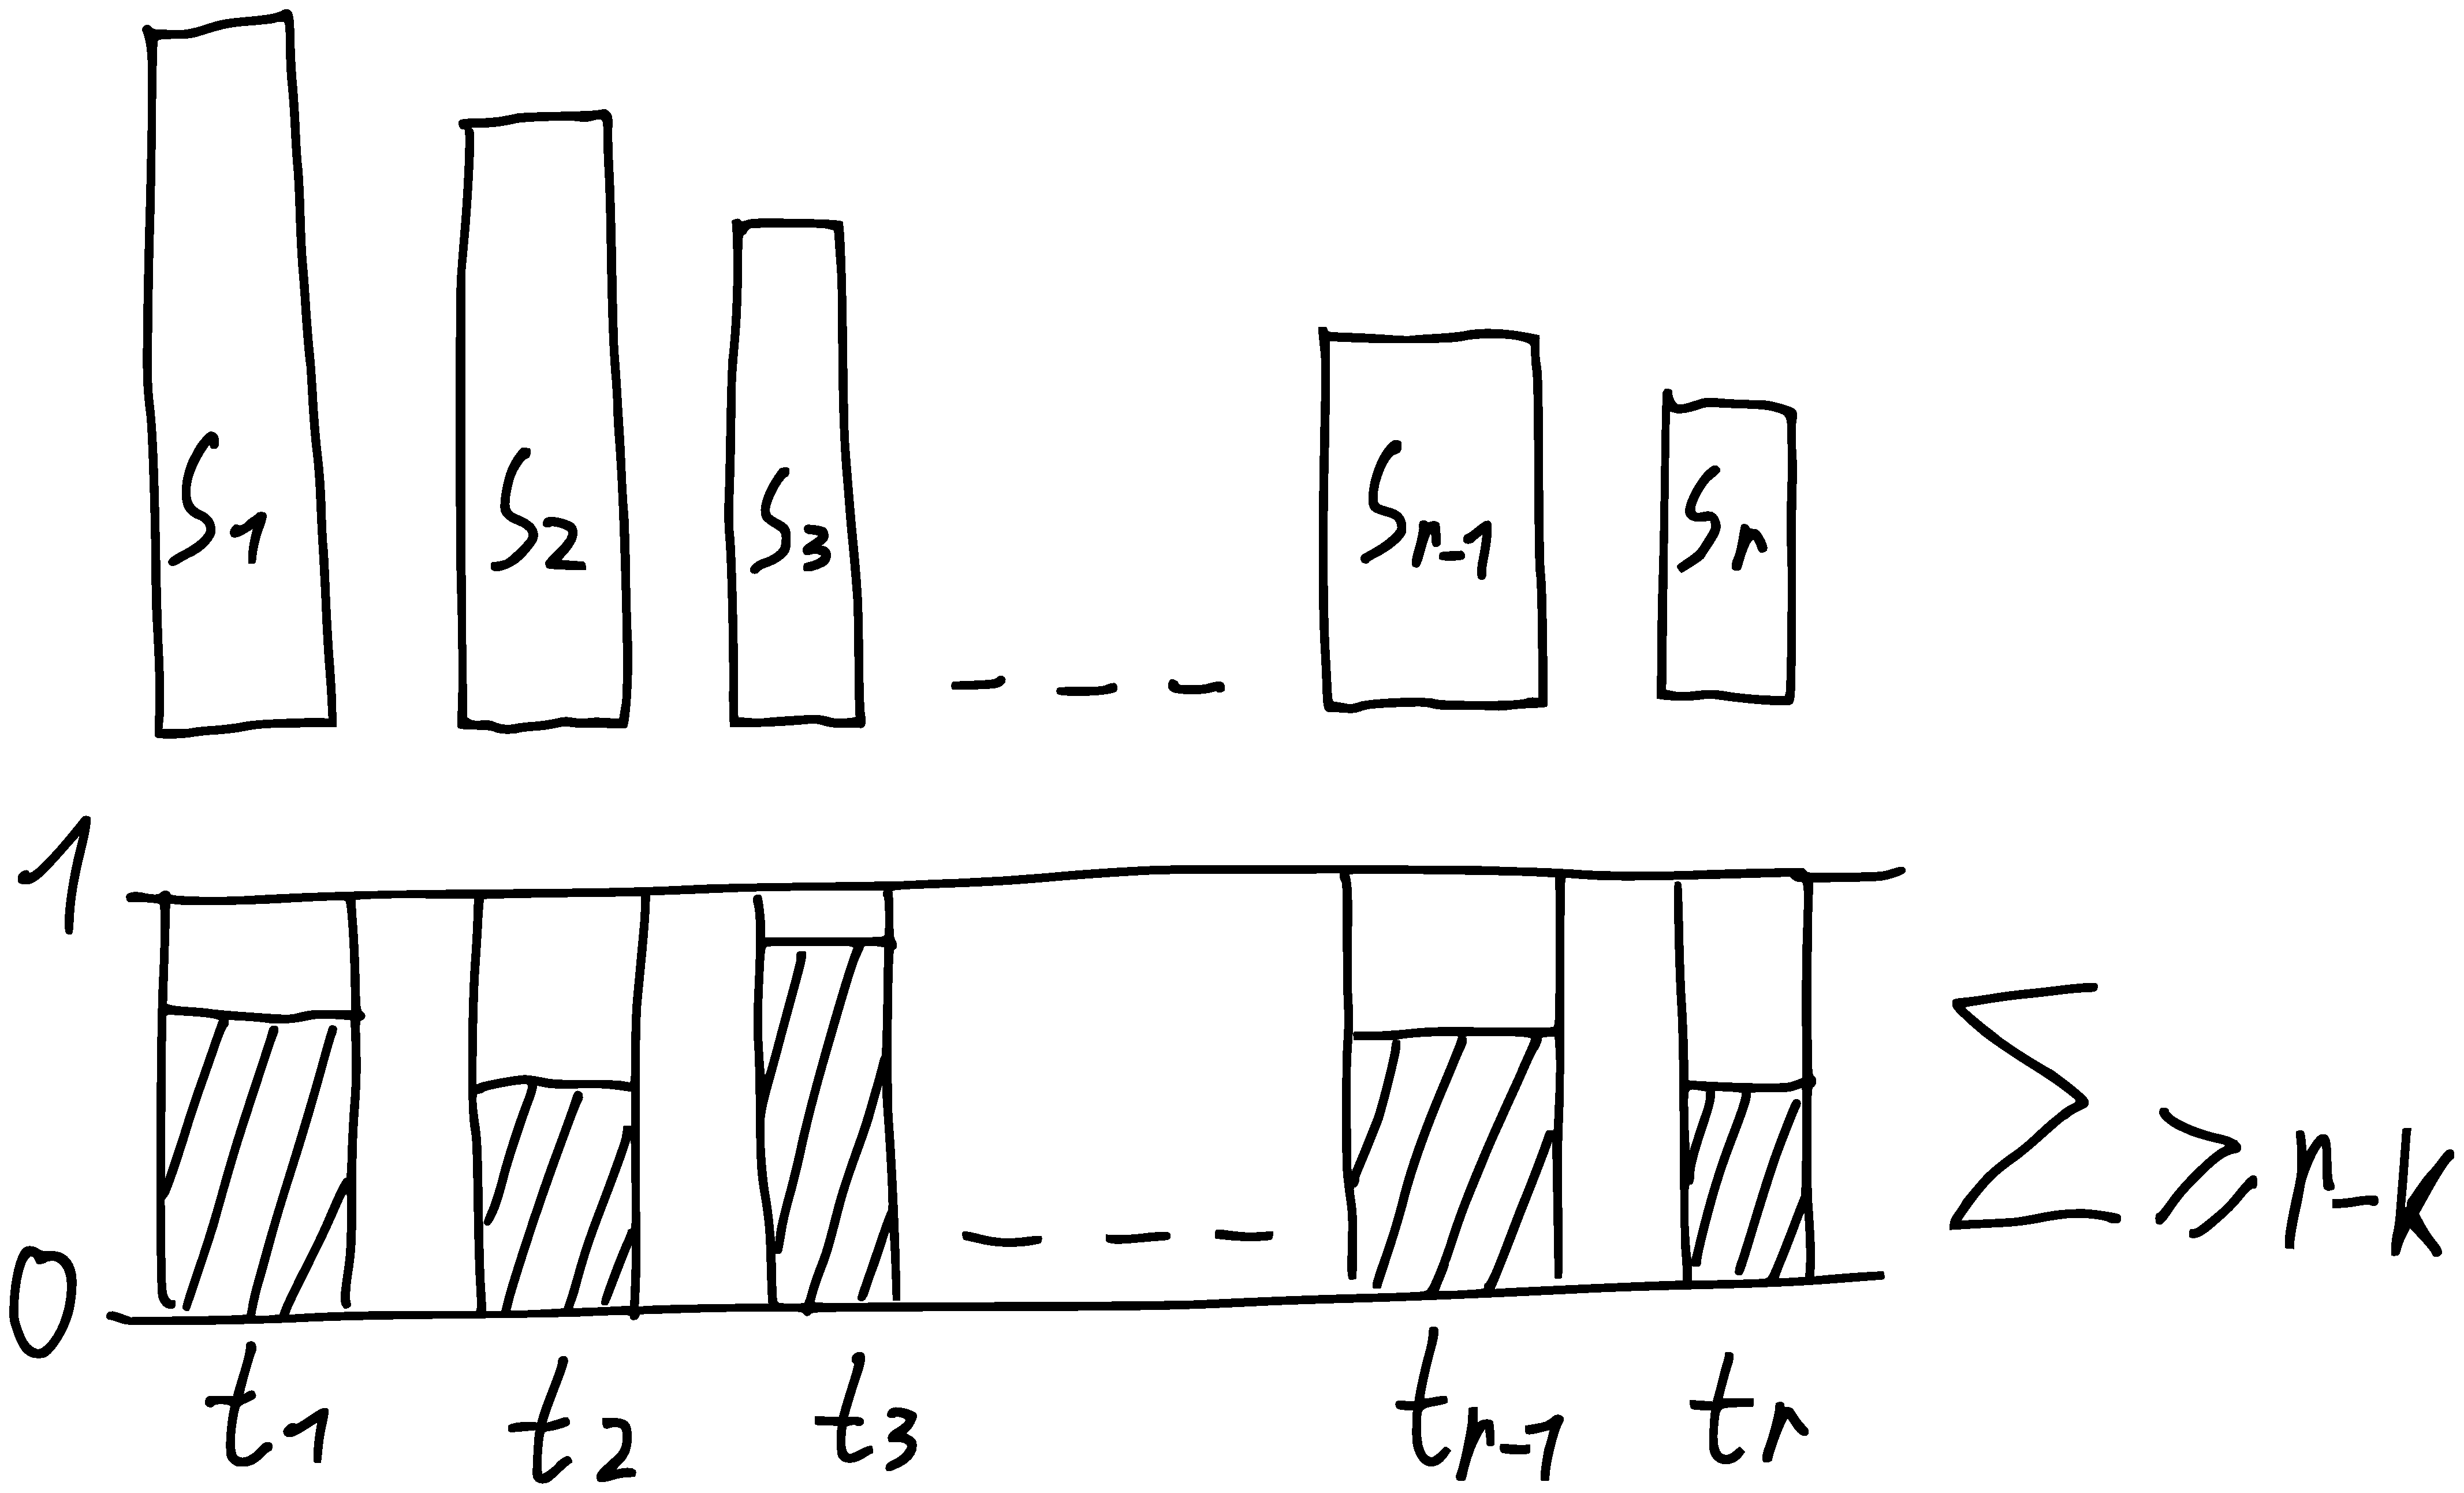
\includegraphics[height=6cm]{img/lecture31_drawing_1}
        \end{center}

        Будем считать сумму как умножение нижней ``колбы'' $0 \leq t_i \leq 1$ на значение сверху $s_i$. То есть изначальная сумма это:
        \begin{equation*}
            s_1 t_1 + \dots + s_{r-1} t_{r-1} + s_r t_r
        \end{equation*}

        Посмотрим на последнюю колбу $t_r$. Если она не полна, возьмем и ``перельем'' в неё содержимое первой колбы так, чтобы она ``заполнилась''. Если она последняя колба не заполнилась от переливания первой, прибаваляем следующие за первой.
        
        Такое переливание уменьшает сумму, так теперь вместо умножения больше $s_1$ на $t_1$ мы будем умножать меньшую $s_r$ на это же $t_1$ перелитое в $t_r$.

        После ``заполнения'' $t_r$, то есть когда она станет равна 1, начинаем таким же образом заполнять $t_{r-1}$ и т.д. Условие гарантирует нам то, что последние $r - k$ колб будут заполнены полностью. Итого, так как полные колбы имеют значение 1, у нас в сумме точно будет будет хотя бы:
        \begin{equation*}
            s_r \cdot 1 + \dots + s_{k+1} \cdot 1. 
        \end{equation*}

        А это в свою очередь по построению меньше изначальной суммы. Это и даёт нам доказываемое неравенство.
        \item[Формальное доказательство со слайдов:] \mbox{}
    
            Индукция по $r$ при фиксированном $k$. При $r = k$ всё верно.

            Пусть теперь $r > k$, так что $r - k \geq 1$.

            По условию имеем $t_1 + \dots + t_{r-1} \geq r - k - t_r \geq 1 - t_r$, поэтому можно подобрать такие числа $\delta_1, \dots, \delta_r$, что 
            \begin{equation*}
                0 \leq \delta_1 \leq t_1, \dots, 0 \leq \delta_{r-1} \leq t_{r-1}  \text{ и } \delta_1 + \dots + \delta_{r-1} = 1 - t_r.
            \end{equation*}
            Для каждого $i = 1, \dots, r-1$ положим $t'_i = t_i - \delta_i$, тогда $0 \leq t'_i \leq 1$. Имеем
            \begin{equation*}
                t'_1 + \dots + t'_{r-1} = t_1 + \dots + t_r - \delta_1 - \dots - \delta_{r - 1} - t_r \geq (r-1) - k
            \end{equation*}
            и тогда по предположению индукции получаем
            \begin{align*}
                & s_1 t'_1 + \dots s_{r-1} t'_{r-1} \geq s_{k+1} + \dots + s_{r-1}, \text{ откуда} \\
                & s_1 t_1 + \dots + s_r t_r = s_1 (t'_1 + \delta_1) + \dots + s_{r-1} (t'_{r-1} + \delta_{r-1}) + s_r t_r = \\
                & = s_1 t'_1 + \dots s_{r-1} t'_{r-1} + s_1 \delta_1 + \dots + s_{r-1} \delta_{r-1} + s_r t_r \geq \\
                & \geq s_1 t'_1 + \dots s_{r-1} t'_{r-1} + s_r (\delta_1 + \dots + \delta_{r-1} + t_r) = \\
                & = s_1 t'_1 + \dots s_{r-1} t'_{r-1} + s_r \geq + s_{k+1} + \dots + s_{r-1} + s_r.
            \end{align*}
    \end{description}
\end{proof}

\begin{proof}[Доказательство теоремы]~
    Так как $\norm{A}$ инвариантна относительнто умножения на ортогональную матрицу слева и справа, достаточно доказать утверждение для случая $A = \Sigma$. Тогда при $B = \Sigma_k$ получаем
    \begin{equation*}
        \norm{\Sigma - B}^2 = \norm{
            \resizebox{5cm}{!}{
                \begin{math}
                \begin{blockarray}{ccccccccccc}
                    \begin{block}{(cccccc|ccccc)}
                    0 & \dots & 0 & 0 & \dots & 0 & & & & &\\
                    \vdots & \ddots & \vdots & \vdots & \ddots & \vdots & & & & &\\
                    0 & \dots & 0 & \vdots & \dots & 0 & & \scaleobj{2}{0} & & &\\
                    0 & \dots & \dots & \sigma_{k+1} & \dots & 0 & & & & &\\
                    \vdots & \ddots & \vdots & \vdots & \ddots & \vdots & & & & &\\
                    0 & \dots & 0 & 0 & \dots & \sigma_r & & & & &\\
                    \cline{1-11}
                    & & & & & & & & & &\\
                    & & & & & & & & & &\\
                    & & \scaleobj{2}{0} & & & & & \scaleobj{2}{0} & & &\\
                    & & & & & & & & & &\\
                    & & & & & & & & & &\\
                    \end{block}
                \end{blockarray}
                \end{math}
            }    
        }^2
        = \sigma_{k+1}^2 + \dots + \sigma_r^2
    \end{equation*}

    Пусть теперь $B \in \text{Mat}_{m \times n} (\RR)$ --- произвольная матрица у словием $\rk B \leq k$. Докажем, что $\norm{\Sigma - B}^2 \geq \sigma_{k+1}^2 + \dots + \sigma_r^2$

    Пусть $\bar{B}$ --- это левый верхний $r \times r$ блок в $B$.

    Пусть $\bar{\Sigma}$ --- это левый верхний $r \times r$ блок в $\Sigma$.

    Тогда $\bar{\Sigma} = \diag(\sigma_1, \dots, \sigma_r) \in M_r (\RR), \enskip \rk \bar{B} \leq \rk B \leq k, \enskip \norm{\Sigma - B}^2 \geq \norm{\bar{\Sigma} - \bar{B}}^2$.

    Положим $S = \langle \bar{B}^{(1)}, \dots, \bar{B}^{(r)} \rangle \subseteq \RR^r, \enskip d = \dim S = \rk \bar{B} \leq k$

    Выберем в $S$ ортонормированный базис $f_1, \dots, f_d$ и дополним его до ортонормированного базиса $f_1, \dots, f_d, f_{d+1}, \dots, f_r$ всего $\RR^r$

    Пусть также $e_1, \dots, e_r$ --- стандартный базис в $\RR^r$ (он ортонормированный). Имеем:
    
    \begin{equation*}
        \norm{\bar{\Sigma} - \bar{B}}^2 = \sum_{i=1}^{r} |\bar{\Sigma}^{(i)} - \bar{B}^{(i)}|^2 \geq \sum_{i=1}^{r} |\ort_S \bar{\Sigma}^{(i)}|^2 = \sum_{i=1}^{r} |\ort_S (\sigma_i \cdot e_i)|^2 = \sum_{i=1}^{r} \sigma_i^2 |\ort_S e_i|^2 = \sum_{i=1}^{r} \sigma_i^2 t_i = \text{\customlabel{lec31:pound}{(\#)}}
    \end{equation*}

    где $t_i = |\ort_S e_i|^2 = |\pr_{S^{\perp}}| \leq 1$, так как $|e_i| = 1$, длина его проекции не больше его длины. Отсюда $0 \leq t_i \leq 1$.

    Тогда, так как $f_{d+1}, \dots, f_r$ --- базис в $S^{\perp}$:
    \begin{equation*}
        t_1 + \dots + t_r = \sum_{i=1}^{r} |\pr_{S^{\perp} e_i}|^2 \overset{\text{\hyperref[lec31:lemma_1]{лемма 1}}}{=} \sum_{i=1}^r \sum_{j=d+1}^r (e_i, f_j)^2 = \sum_{j=d+1}^r \sum_{i=1}^r (e_i, f_j)^2 \overset{\text{\hyperref[lec31:lemma_1]{лемма 1}}}{=} \sum_{j=d+1}^r \underbracket{|f_j|^2}_{=1} = r - d \geq r - k
    \end{equation*}

    Тогда по \hyperref[lec31:lemma_2]{лемме 2}:  \ref{lec31:pound} $\geq \sigma_{k+1}^2 + \dots + \sigma_r^2$

    Подытожим:
    \begin{equation*}
        \norm{\Sigma - B}^2 \geq \norm{\bar{\Sigma} - \bar{B}}^2 \geq \sigma_{k+1}^2 + \dots + \sigma_r^2 = \norm{\bar{\Sigma} - \bar{\Sigma_k}}^2
    \end{equation*}

    $\forall B$ ранга $\leq k$.
\end{proof}

\begin{exercise}
    $A = U \Sigma V^T, B = U \Sigma_k V^T$ --- наилучшее приближение ранга $\leq k \implies B = U_k \cdot  U_k^T \cdot A$, где $U_k = (u_1 | \dots | u_k) \in \text{Mat}_{m \times k} (\RR)$
\end{exercise}


\end{document}
